%  Manuscrito para Forecasting (MDPI) -- plantilla oficial mdpi.cls
%  Estructura: main.tex + secciones/*.tex + referencias.bib + figuras/
%  BASE EXPERIMENTAL: experimento v2 rolling-origin (2021--2025, 10 modelos).
%  Las cifras del experimento LATINCOM / v1 y del borrador provincial estan DESCARTADAS.
%  Todo el manuscrito va en ingles (decision 30-10-2026).
%  listo12 (31-10-2026): URL del repo con mayusculas exactas.
%  listo11 (31-10-2026): Discusion reescrita con el informe de Opus (cifras verificadas contra CSV);
%  Holm, sensibilidad 2023--2025, DM vs bootstrap, RMSE/MASE, reproducibilidad (Excel no redistribuido).
%  listo10 (31-10-2026): TimesFM/Moirai verificados (PMLR 235); tag v2.0-forecasting.
%  listo9 (31-10-2026): citas a todas las tablas/figuras, KPSS 2023--2025, empates P75,
%  sensibilidad 2023--2025 de la ablacion, YoY robusto, \ref a Transparency.
%
%  CORRECCIONES DE CITAS (30-10-2026):
%   - Claves alineadas con el .bib: gu2022forecasting, yin2020stl, bao2025study,
%     ray2024arima, avinash2024hidden, nayak2024exogenous, zhao2025hybrid,
%     perez2021pysentimiento, hochreiter1997lstm, bahdanau2015neural,
%     chen2016xgboost, hyndman2006another, diebold1995comparing,
%     harvey1997testing, lundberg2017unified.
%   - Citas nuevas: das2024decoder, woo2024unified, perez2022robertuito,
%     dickey1979distribution, kwiatkowski1992testing, kingma2015adam,
%     tashman2000out, holm1979simple, efron1993bootstrap.
%   - Claves sin entrada en el .bib (sabo2023, chergui2022, praveenkumar2025,
%     ryu2020, an2024, paudel2023, firat2026, jauhar2025) reemplazadas por
%     articulos que si estan: rather2024breaking, hewamalage2023forecast,
%     manogna2025enhancing, choudhary2025genetic, sediyono2025integrated,
%     chong2022using, du2024financial, rosa2025brazilian, jahin2025mcdfn,
%     bourday2026explainable.
%   - \bibliography apunta a referencias.bib.
\documentclass[forecasting,article,submit,moreauthors]{Definitions/mdpi}

\usepackage[utf8]{inputenc}
\usepackage{amsmath}
% --- Paquete de figuras y tablas v2 ---
\graphicspath{{figuras/}{figures/}}
\usepackage{booktabs}
\usepackage{subcaption}
\captionsetup[subfigure]{labelformat=empty}
\usepackage{longtable}
\usepackage{pdflscape}
% Marca visible para todo lo que aun debe ejecutarse o confirmarse:
\newcommand{\pendiente}[1]{\textcolor{red}{[PENDIENTE: #1]}}
% Recordatorio de lo que exige el formato y ya se cumple (borrar antes del envio):
\newcommand{\formato}[1]{\textcolor{red}{[FORMATO, cumplido: #1]}}
% Inserta la figura si el archivo existe; si no, deja un recuadro rojo con el nombre.
\newcommand{\figura}[2]{\centering\IfFileExists{#1.png}{\includegraphics[width=#2]{#1.png}}{\fbox{\parbox{0.8\textwidth}{\centering\pendiente{falta el archivo \detokenize{#1}.png}}}}}

\firstpage{1}
\makeatletter
\setcounter{page}{\@firstpage}
\makeatother
\pubvolume{1}
\issuenum{1}
\articlenumber{0}
\pubyear{2026}
\copyrightyear{2026}
\datereceived{ }
\daterevised{ }
\dateaccepted{ }
\datepublished{ }

\Title{Deterioration under Abrupt Production Changes: Evaluating a DualLSTM with Bahdanau Attention against Statistical and Pretrained Benchmarks for Peruvian Agro-Industrial Forecasting under Small Data}
% \pendiente{t\'itulo provisional (opci\'on A); confirmar con el asesor.}

\Author{Fabrizio Yerald Alfonso Sanchez Saravia $^{1}$, Alex Coila Jarita $^{1}$ and Esteban Tocto-Cano $^{1,}$*}
\AuthorNames{Fabrizio Yerald Alfonso Sanchez Saravia, Alex Coila Jarita and Esteban Tocto-Cano}

\address{%
$^{1}$ \quad Professional School of Systems Engineering, Faculty of Engineering and Architecture, Universidad Peruana Uni\'on, Juliaca, Peru}

\corres{Correspondence: estocan@upeu.edu.pe}

\abstract{Averaged forecast error can hide how models behave at abrupt production changes, which matters in short agricultural series. We evaluate a dual-branch LSTM with Bahdanau attention (DualLSTM), which processes the production history and a lagged exogenous context (climate, emergencies and news sentiment) separately, for one-step-ahead forecasts of national monthly production of sour lime and sweet lime in Peru. Under a leakage-controlled rolling-origin design with test years 2021--2025 (60 months per crop), it is compared with eight benchmarks, including the pretrained Chronos-Bolt-tiny, using the mean absolute error (MAE) over all months and over shock months (monthly P75 threshold) and the relative shock penalty $\Delta_s$. For sour lime, Chronos had the lowest MAE (2,649~t; 95\% CI 2,171--3,144), whereas the two DualLSTM variants had the highest (6,361 and 6,744~t). For sweet lime, SARIMA was the best model (18.4~t) and the only one ranked first or tied at all four thresholds. The DualLSTM showed low $\Delta_s$ (sour lime: $-4.5$\% and 1.2\%) only together with high absolute errors, and news features gave no clear benefit. $\Delta_s$ should therefore be reported together with absolute errors, and greater model complexity did not reduce the error with few data.}

\keyword{agro-industrial forecasting; small data; DualLSTM; Bahdanau attention; abrupt production changes; shock-conditional evaluation; pretrained time-series models}

\begin{document}

% ============================================================
\section{Introduction}

Forecasting monthly agricultural production is necessary to plan supply, logistics and prices, but in many countries the available series are short, strongly seasonal and subject to abrupt changes associated with climatic events, emergencies or market disruptions. With so little data, greater model complexity does not guarantee better out-of-sample performance: forecasting competitions and reviews of recurrent networks show that statistical and parsimonious methods remain hard benchmarks to beat~\cite{makridakis2020m4,makridakis2022m5,hewamalage2021rnn,lim2021timeseries}, and it has been questioned whether deep architectures outperform simpler alternatives when data are scarce~\cite{rather2024breaking,hewamalage2023forecast}.

At the same time, the agricultural forecasting literature has proposed LSTM networks with attention mechanisms, hybrid models and boosting that incorporate meteorological and other exogenous variables~\cite{gu2022forecasting,yin2020stl,bao2025study,manogna2025enhancing,choudhary2025genetic,sediyono2025integrated,ray2024arima,avinash2024hidden,nayak2024exogenous,zhao2025hybrid,chandan2025exogenous,celik2025hybrid}. Indicators derived from news and the integration of heterogeneous sources have also been used as auxiliary information~\cite{lukauskas2022economic,chong2022using,liapis2023investigating,du2024financial,rosa2025brazilian}. However, many of these studies use longer series, compare against few simple benchmarks, or evaluate only the average error, without examining what happens in the months of abrupt change, which are those of greatest operational interest. In addition, pretrained time-series models such as Chronos~\cite{ansari2024chronos}, TimesFM~\cite{das2024decoder} and Moirai~\cite{woo2024unified} offer a new benchmark that can forecast without local training.

This work extends a preliminary study presented at IEEE LATINCOM 2026~\cite{sanchez2026latincom}. It evaluates a DualLSTM architecture with Bahdanau attention that explicitly separates the production history from the lagged exogenous context. The aim is not to demonstrate the superiority of the architecture, but to measure, under a protocol that controls information leakage, how it compares with statistical, regularised, tree-based and pretrained benchmarks on two Peruvian national series: sour lime and sweet lime. The research questions are:
\begin{enumerate}
\item Does the DualLSTM with attention outperform simpler and pretrained benchmarks in overall forecast error with few data?
\item Do the conclusions hold when the evaluation is restricted to months of abrupt change?
\item Do variables derived from news text improve forecast accuracy?
\end{enumerate}

The contributions are: (i) a reproducible rolling-origin evaluation of a dual-branch recurrent architecture against eight benchmarks on two crops; (ii) an analysis conditioned on abrupt changes, with a threshold defined only from information available at the forecast origin and its sensitivity; (iii) a multi-seed evaluation without selection of the best seed; and (iv) an explicit account of which parts of the protocol were fixed after seeing earlier results, so that the evidence is not over-read.

% =====================================================================
% Materials and Methods, rolling-origin experiment (v2). Draft 1.
% Source of every statement: Opus read-only report of 2026-10-29
% (DECISIONES_METODOLOGICAS.md, 01_configuracion/*.json, manifest.json).
% No result figures appear here. \pendiente{...} = still to be confirmed.
% Citation keys: those already used in main.tex; entries missing in
% referencias.bib print as [?] until ChatGPT/Scopus verification.
% =====================================================================
\section{Materials and Methods}\label{sec:methods}

\subsection{Study design}
We evaluate one-step-ahead forecasts of monthly national production of two crops, sour lime (\textit{lim\'on sutil}) and sweet lime (\textit{lim\'on dulce}), in Peru, using a rolling-origin design~\cite{tashman2000out} (Figure~\ref{fig:fig_workflow}). For each test year $Y\in\{2018,\dots,2025\}$ the forecast origin is December of $Y-1$: models are fitted with data up to December of $Y-2$, tuned and early-stopped on year $Y-1$, and produce twelve one-step-ahead forecasts for year $Y$ (Figure~\ref{fig:fig30_rolling_origin_scheme}). Lagged values of the test year are taken from observations, as is usual in one-step-ahead evaluation. All models share the same partitions in every window.

Trained models require at least 36 training months. Windows 2018--2020 therefore include only the three models that need no training (Naive, Seasonal Naive and Chronos), which gives 118 viable model--window--crop combinations and 42 that do not apply. The primary ranking pools the windows 2021--2025; a sensitivity analysis repeats all conclusions on 2023--2025.

\begin{figure}[H]
\centering
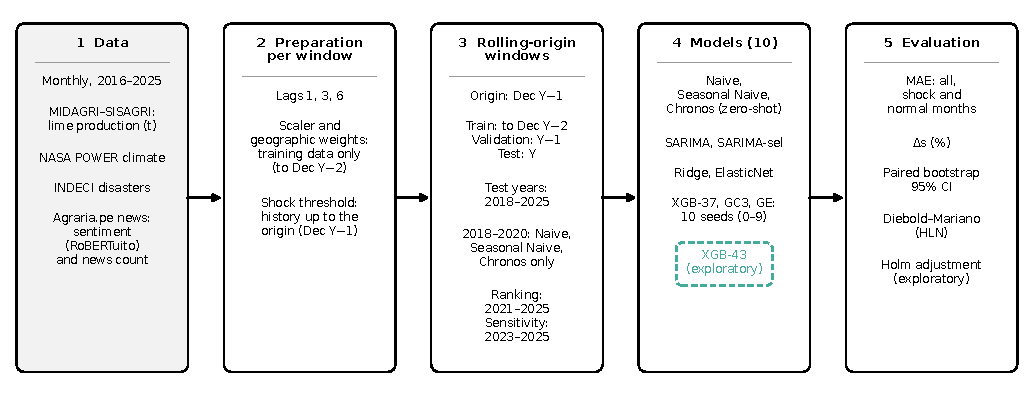
\includegraphics[width=\textwidth]{fig_workflow.pdf}
\caption{Study workflow: data sources, preparation within each window, rolling-origin windows, models and evaluation. The dashed box marks the exploratory XGB-43 model, which is outside the ranking.\label{fig:fig_workflow}}
\end{figure}

\subsection{Data}
The national series of each crop is the sum of monthly provincial production recorded by MIDAGRI--SISAGRI~\cite{midagri2026perfil} from January 2016 to December 2025 (109 provinces with a record of at least one of the two crops; Figure~\ref{fig:fig29_study_area_map} and Table~\ref{tab:S1_provinces}). Exogenous variables enter the models only with lags of 1, 3 and 6 months.
\begin{itemize}
\item \textbf{Climate:} NASA POWER monthly values at the coordinates of the 109 provinces: mean (T2M) and maximum (T2M\_MAX) temperature, wind speed (WS2M), precipitation (PRECTOTCORR) and relative humidity (RH2M). Units: temperature in $^{\circ}$C (T2M is the monthly mean and T2M\_MAX the monthly mean of the daily maximum), wind speed in m\,s$^{-1}$, precipitation in mm\,day$^{-1}$ (monthly mean of daily totals, not a monthly sum) and relative humidity in \%.  No values were missing and no imputation was applied. Ten provinces use the reference coordinate of their department.
\item \textbf{Emergencies:} the official INDECI emergency records, restricted to ten climate-related hazards (heavy rain, strong winds, low temperatures, flood, landslide, mudflow, drought, erosion, thunderstorm and swell). Five monthly series are used: number of emergencies, people affected, people homeless, and hectares of crop lost and affected. Months without records are coded as zero. The conversion of the raw INDECI records into this monthly panel, including the zero coding, has no associated code in the repository (see Reproducibility).
\item \textbf{News sentiment:} 2,883 news items from the agribusiness section of Agraria.pe. The sentiment of each item is $s=P(\text{positive})-P(\text{negative})$ from the RoBERTuito model of \texttt{pysentimiento}~\cite{perez2022robertuito,perez2021pysentimiento}, applied zero-shot to the headline and the first 200 words. Two monthly series are built (mean sentiment and number of items); months without news (January and February 2016) are set to zero.
\end{itemize}
Provincial climate and emergency series are aggregated to national level with fixed, crop-aware geographic weights estimated only on the training period of each window. When a province has no records, the aggregator renormalises over the weight mass present. Lags are computed on the already aggregated national series.

Table~\ref{tab:main_descriptive_series} summarises the series of each window, with the ADF~\cite{dickey1979distribution} and KPSS~\cite{kwiatkowski1992testing} unit-root and stationarity tests.

\subsection{Shock definition}
For each month the absolute month-on-month relative change is
\begin{equation}
r_t=\left|\frac{y_t-y_{t-1}}{y_{t-1}}\right|,
\label{eq:shock}
\end{equation}
and the year-on-year version replaces $y_{t-1}$ by $y_{t-12}$. A month of the test year is a \textit{shock} if $r_t>P_k$, where $P_k$ is the linear-interpolation percentile of the changes dated from the start of the series up to the forecast origin. The primary definition is the 75th percentile (P75) of the month-on-month change; P50, P60 and P90, and the year-on-year version, are reported as sensitivity points, and a full sweep from P0 to P95 is computed. P0 (every month is a shock) is used as a code check, because $\Delta_s$ must equal exactly zero there. A window with fewer than two shock months is flagged as non-informative, but its months are kept in the pooled estimates. The definition is statistical and attributes no cause.

\subsection{Models}
Ten models are ranked (Table~\ref{tab:main_models}).
\begin{table}[H]
\caption{Models in the ranking. Seeded models use ten seeds (0--9).\label{tab:main_models}}
\newcolumntype{C}{>{\raggedright\arraybackslash}X}
\begin{tabularx}{\textwidth}{lC}
\toprule
\textbf{Model} & \textbf{Description}\\
\midrule
Naive, Seasonal Naive & $\hat y_t=y_{t-1}$ and $\hat y_t=y_{t-12}$\\
SARIMA & Fixed order, one-step updating without re-estimation~\cite{box2015time}\\
SARIMA-sel & Order selected in each window (see below)\\
Chronos & Pretrained Chronos-Bolt-tiny~\cite{ansari2024chronos}, zero-shot, univariate\\
Ridge, ElasticNet & Regularised linear models with 37 predictors~\cite{zou2005regularization}\\
XGB-37 & Gradient boosting with the same 37 predictors~\cite{chen2016xgboost}\\
GC3 & Dual-LSTM with attention, 37 predictors (no news)\\
GE & GC3 plus six lagged news features\\
\bottomrule
\end{tabularx}
\end{table}

\textbf{Benchmarks without training.} Chronos uses \texttt{amazon/chronos-bolt-tiny} with the median forecast, horizon 1 and the full univariate history from January 2016 up to $t-1$. Its comparison with the multivariate models concerns predictive performance, not equal information sets.

\textbf{SARIMA.} The fixed orders are $(1,1,1)(1,1,0)_{12}$ for sour lime and $(1,0,0)(0,1,0)_{12}$ for sweet lime, both with a constant term, seasonal period 12 and one-step-ahead updating without re-estimating parameters. For SARIMA-sel, a grid of 576 orders ($p\in0..3$, $d\in0..1$, $q\in0..3$, $P\in0..2$, $D\in0..1$, $Q\in0..2$, $m=12$) is fitted on the training months; the five orders with the lowest AIC are refitted, and the one with the lowest one-step-ahead MAE on year $Y-1$ is kept.

\textbf{Ridge and ElasticNet.} The penalty $\alpha\in\{0.001,0.01,0.1,1,10,100\}$ and, for ElasticNet, the mixing ratio $\{0.2,0.5,0.8\}$ are re-chosen in each window by the validation MAE in tonnes; ties are resolved in favour of the first grid entry. The final fit uses the training months only. Predictors are standardised with the training mean and standard deviation.

\textbf{XGB-37.} Squared-error gradient boosting with maximum depth 2, learning rate 0.05, 200 trees, subsample 0.8 and column subsample 0.8, with default regularisation and no hyperparameter search. The 37 predictors are the four production variables (current production and its lags 1, 3 and 6), three calendar terms (sine and cosine of the month and a time index), and the five climate and five emergency series at lags 1, 3 and 6.

\textbf{Dual-LSTM with attention (GC3 and GE).} Two recurrent branches process the previous six months (Figure~\ref{fig:fig25_architecture_dual_lstm}). Branch A receives the four production variables and branch B the calendar, climate and emergency variables (33 features in GC3; 39 in GE, which adds mean sentiment and news count at lags 1, 3 and 6). Each branch has a 16-unit LSTM~\cite{hochreiter1997lstm} followed by additive Bahdanau attention~\cite{bahdanau2015neural} of 16 units; the context vectors are concatenated and passed through dense layers of 16 and 8 units (ReLU), dropout 0.20 and a scalar output. GC3 has 6,273 and GE 6,657 trainable parameters. Training uses Adam~\cite{kingma2015adam} (learning rate 0.001), mean-squared-error loss, batch size 8, up to 300 epochs, no shuffling, early stopping on the validation year (patience 15, best weights restored) and learning-rate reduction on plateau (factor 0.5, patience 8). No hyperparameter search was run.

\textbf{Seeds.} XGB-37, GC3 and GE are trained with ten seeds (0--9) and no seed is selected. The error series of a seeded model is the monthly mean of the absolute errors over its seeds, and seed dispersion is reported separately. Each network run starts in a new process with deterministic settings.

\textbf{Exploratory model.} XGB-43 adds the six lagged news features to XGB-37 with the same hyperparameters. It was added post hoc, is not part of the ranking, the Diebold--Mariano tests or the multiplicity correction, and appears only in the exploratory comparison with XGB-37.

\subsection{Leakage control}
Within each window, the scaler, the geographic weights, the hyperparameters that are re-chosen (Ridge, ElasticNet, SARIMA-sel) and the MASE denominator use data up to December of $Y-2$ only, and the shock threshold uses the history up to the forecast origin (December of $Y-1$). Early stopping and model selection use year $Y-1$, never the test year. An automated test checks these conditions.

\subsection{Evaluation}
The main metric is the mean absolute error (MAE, in tonnes) over all test months, over the shock months and over the remaining (normal) months. The relative shock penalty is
\begin{equation}
\Delta_s=\frac{\mathrm{MAE}_{\text{shock}}-\mathrm{MAE}_{\text{all}}}{\mathrm{MAE}_{\text{all}}}\times 100.
\label{eq:deltas}
\end{equation}
Because $\Delta_s$ is a ratio, it can be low either because the shock error is small or because the normal-month error is large; it is therefore always reported together with $\mathrm{MAE}_{\text{shock}}$ and $\mathrm{MAE}_{\text{normal}}$. We also compute the RMSE, the ratio of shock to normal MAE, $\Delta_s$ when each shock month is removed in turn, the MAE by quartile of $|\Delta y/y|$, and the MASE with a single denominator per window~\cite{hyndman2006another}, the mean of $|y_t-y_{t-12}|$ over the training months of that window (undefined in 2018). These secondary metrics are provided, without confidence intervals, in the metric tables of the repository. A model is called best if it ranks first, or ties with the first, in at least three of the four reporting thresholds P50, P60, P75 and P90 for a crop.

\textbf{Uncertainty.} Confidence intervals come from a paired bootstrap~\cite{efron1993bootstrap} over months with the same indices for all models, stratified by window ($B=10{,}000$, seed 42, 2.5th and 97.5th percentiles). For $\mathrm{MAE}_{\text{shock}}$ and $\mathrm{MAE}_{\text{normal}}$, months are resampled within their own type. A sensitivity analysis uses circular moving blocks of three months. A model ties with the first if the interval of its difference with the first contains zero.

\textbf{Significance tests.} Pairs of models are compared with the Diebold--Mariano test with the Harvey--Leybourne--Newbold correction~\cite{diebold1995comparing,harvey1997testing} ($h=1$, absolute loss, seed-averaged errors, pooled windows 2021--2025, two-sided $t_{n-1}$), on all months and on shock months only. With few shock months, power is low. As an exploratory addition, p-values are adjusted by the Holm method~\cite{holm1979simple} within each family (crop $\times$ subset, 45 pairs).

\textbf{Fit diagnostics.} A model--window is flagged as overfitted if the ratio of validation to training MAE exceeds 2.0; the same ratio for the Naive forecast is shown for reference.

\subsection{Transparency about the protocol}\label{sec:transparency}
The protocol was written down before the rolling-origin experiment was run, but the test year 2025 had already been inspected in earlier experiments of this project. The hyperparameters of GC3, GE and XGB-37 were fixed with data up to 2024, and the order of the fixed sour-lime SARIMA was adopted after observing the 2025 results. Windows 2021--2024 are therefore retrospective evaluations, not independent test sets. We report these facts so that the 2025 window is not read as a confirmatory test.

\subsection{Reproducibility}
All experiments ran on CPU only (Windows 11 Pro; AMD64 family 25, model 33 processor with 16 logical cores) with Python 3.11.9, TensorFlow 2.21.0, Keras 3.14.0, statsmodels 0.14.6, xgboost 3.2.0, scikit-learn 1.8.0, torch 2.11.0 (CPU) and chronos-forecasting 2.3.2, with \texttt{pysentimiento} 0.7.3. Environment variables fix the hash seed and deterministic operations, the global seed is 42, and the SHA-256 hashes of the frozen input tables are stored with the code. Everything from the frozen tables to the final metrics is reproducible with a single driver script. Three links of the data chain have no code in the repository and are provided as frozen tables: the processing of the MIDAGRI--SISAGRI spreadsheet into national series, the processing of the INDECI records into the monthly panel, and the province coordinates. The news corpus and the NASA POWER values can change if collected again. Code and frozen tables: \texttt{https://github.com/YeralD21/Machine-Learning-Multimodal--Agro-NLP-Clima-}, release \texttt{v2.0-forecasting}. The MIDAGRI--SISAGRI table was downloaded from the Regional Productive Profile dashboard on 25 June 2026 (the file covers February 2015 to March 2026; this study uses January 2016 to December 2025); because the dashboard is updated monthly and past figures may be revised, the national series derived from it are provided in the repository as frozen tables, and the SHA-256 hash of the downloaded spreadsheet is recorded with the code. The spreadsheet itself (229~MB) is not redistributed. It was exported in consecutive sheets of at most 1,048,001 rows; we checked that the number of lime records per year in the spreadsheet matches the derived tables for 2016--2025, so the export was not truncated.

% ============================================================
% 3. RESULTADOS
% Fuente: REGISTRO_MAESTRO_RESULTADOS.md, secciones 5--9.
% GC3, GE y XGB-37: media de las metricas por semilla (estimando a).
% ============================================================

\section{Results}

\subsection{Series and overall accuracy}
Table~\ref{tab:main_descriptive_series} describes the series by window. Sour lime production averages between 23,067 and 32,209~t per month in the test years, with a coefficient of variation of 0.16--0.36, and sweet lime between 394 and 468~t, with 0.36--0.39. The unit-root tests are not conclusive: for sour lime the ADF test rejects a unit root in 2021--2023 but not in 2024--2025, and the KPSS test rejects level stationarity in 2023--2025, and for sweet lime neither test rejects its null in any window. Figure~\ref{fig:fig24_series_with_shocks} shows the series and the shock months.

Table~\ref{tab:main_aggregate_accuracy} gives the pooled accuracy over the 60 test months of 2021--2025. For sour lime, Chronos had the lowest MAE (2,649~t; 95\% CI 2,171--3,144), followed by SARIMA-sel (3,206~t), SARIMA (3,361~t) and the Naive forecast (3,624~t). GC3 and GE had the highest errors of the ten models (6,361 and 6,744~t), above the Seasonal Naive (6,075~t). For sweet lime, SARIMA had the lowest MAE (18.4~t; 14.5--22.8), followed by SARIMA-sel (20.6~t) and the Seasonal Naive (24.5~t), whereas GC3 and GE both reached 56.7~t, above Ridge, ElasticNet and XGB-37 (48.3--53.1~t). Figure~\ref{fig:fig20_real_vs_pred_2025} shows the 2025 forecasts, and Figure~\ref{fig:fig20_real_vs_pred_2023_sutil__fig20_real_vs_pred_2024_dulce} those of 2023 for sour lime and 2024 for sweet lime. The MAE of each test window is given in Tables~\ref{tab:T05_MAE_P75_por_ventana_sutil} and~\ref{tab:T05_MAE_P75_por_ventana_dulce}, and the monthly absolute errors in Figure~\ref{fig:fig21_abs_error_monthly}.

\subsection{Shock months}
With the monthly P75 threshold, the pooled sample contains 10 shock months for sour lime and 15 for sweet lime (Figure~\ref{fig:fig10_n_shock_heatmap_window_percentile}; the number of shock months at each percentile is shown in Figure~\ref{fig:fig09_n_shock_vs_percentile}). In sour lime, Chronos also had the lowest MAE in shock months (4,784~t), and SARIMA-sel and the Seasonal Naive ranked second and third (Table~\ref{tab:main_robust_ranking}); GC3 ranked sixth and GE seventh. In sweet lime, SARIMA ranked first (14.0~t), with the Seasonal Naive third, GE fifth and GC3 sixth. The intervals for shock months are wide (for example 2,259--7,928~t for the Seasonal Naive in sour lime; Figure~\ref{fig:fig11_bootstrap_ci_mae_shock_report_points}), so in sour lime five models are statistically tied with Chronos at P75, whereas in sweet lime no model is tied with SARIMA (asterisks in Table~\ref{tab:main_robust_ranking}). Shock-month errors by window are given in Tables~\ref{tab:T05_MAE_shock_P75_por_ventana_sutil} and~\ref{tab:T05_MAE_shock_P75_por_ventana_dulce} and Figure~\ref{fig:fig14_mae_shock_heatmap_model_window}, and the rank of each model by window in Figure~\ref{fig:fig08_rank_bump_chart}.

The penalty $\Delta_s$ must be read together with the absolute errors (Table~\ref{tab:main_aggregate_accuracy}, Figure~\ref{fig:fig13_mae_normal_vs_shock_bars}). In sour lime, the Seasonal Naive had $\Delta_s=-17.1$\% and GC3 $-4.5$\%, but both had a high MAE in all months, so their shock error was not low in absolute terms: Chronos, with $\Delta_s=80.6$\%, had a lower shock MAE than either. In sweet lime, SARIMA combined the lowest shock error with $\Delta_s=-24.1$\%, GC3 and GE had $\Delta_s$ of 7.2\% and 2.0\%, and the Seasonal Naive had $\Delta_s=0.0$\%. The ratio of shock to normal MAE (Figure~\ref{fig:fig06_ratio_shock_normal_vs_percentile}), the MAE by quartile of the monthly change (Figure~\ref{fig:fig16_mae_by_change_quartile}) and $\Delta_s$ when each shock month is removed in turn (Figure~\ref{fig:fig17_leave_one_shock_out_delta_s}) are reported as complementary diagnostics.

A model is robust if it is first or tied in at least three of the four thresholds P50, P60, P75 and P90 (Table~\ref{tab:main_robust_ranking}; Figures~\ref{fig:fig04_delta_s_vs_percentile}, \ref{fig:fig05_mae_shock_vs_percentile} and \ref{fig:fig07_rank_heatmap_model_percentile}). With the month-on-month definition, Chronos, SARIMA and SARIMA-sel were robust in sour lime, and only SARIMA in sweet lime. Neither GC3 nor GE was robust in either crop. With the year-on-year definition (Table~\ref{tab:main_robust_ranking}, Figure~\ref{fig:fig12_yoy_vs_mom_threshold}), the robust models were the Naive forecast and Chronos in sour lime, and Chronos, SARIMA and SARIMA-sel in sweet lime; GC3 and GE were again not robust.

\subsection{Statistical comparisons}
Tables~\ref{tab:T09_DM_matriz_principal_2021_2025_sutil} and~\ref{tab:T09_DM_matriz_principal_2021_2025_dulce} report the Diebold--Mariano tests with the Harvey--Leybourne--Newbold correction (unadjusted $p$-values, also shown in Figure~\ref{fig:fig19_dm_pvalue_matrix}; Holm-adjusted values in Figure~\ref{fig:fig19b_dm_pvalue_matrix_holm}, exploratory). On all months of sour lime, GC3 and GE had significantly larger errors than Chronos, SARIMA, SARIMA-sel and XGB-37 ($p\le0.001$). With only 10 shock months, the only comparisons with $p<0.05$ involved the Naive forecast. In sweet lime, SARIMA had a significantly lower error than every model except SARIMA-sel on all months ($p=0.20$ against SARIMA-sel), and on the 15 shock months it was significantly better than every other model ($p\le0.001$) except SARIMA-sel ($p=0.115$). Power is limited in all shock-only comparisons. After the exploratory Holm adjustment, the number of pairs with $p<0.05$ fell from 28 to 17 (sour lime, all months), from 4 to 1 (sour lime, shock months; only Chronos against the Naive forecast), from 33 to 28 (sweet lime, all months) and from 31 to 24 (sweet lime, shock months). The advantage of SARIMA over SARIMA-sel was not significant in any subset, and its advantage over the Seasonal Naive in sweet lime did not survive the adjustment on all months ($p_{\text{Holm}}=0.070$) but did on shock months ($p_{\text{Holm}}=0.018$).

\subsection{Contribution of news features}
Table~\ref{tab:T11_ablacion_sutil} and Table~\ref{tab:T11_ablacion_dulce} (Figure~\ref{fig:fig18_nlp_ablation_paired}) compare GE with GC3, seed by seed. In sour lime, adding the news features increased the pooled error by 382~t (95\% CI 45--711), and GE was better than GC3 in only one of ten seeds; the Diebold--Mariano test on the seed-averaged errors gave $p=0.061$. In sweet lime the difference was 0.1~t (95\% CI $-1.9$ to 1.9), with no evidence of an effect over all months; in shock months it was $-2.9$~t ($-6.2$ to 0.7). In the 2023--2025 sensitivity set, the sour-lime difference remained positive (601~t; 89 to 1,096), whereas in sweet lime GE had a lower shock-month error than GC3 ($-4.3$~t; $-7.2$ to $-1.5$; 9 months), although the Diebold--Mariano test on the seed-averaged errors did not separate them ($p=0.319$). The two procedures answer different questions (the paired seed-by-seed difference versus the difference between seed-averaged forecasts), so neither result is read as evidence of an effect of the news features. The exploratory comparison of XGB-43 with XGB-37 (Table~\ref{tab:T16_exploratorio_xgb43} and Figure~\ref{fig:fig18b_xgb43_vs_xgb37_exploratory}; post hoc, outside the ranking) found a higher error in sour lime (130.5~t; CI 1.5--260.4) and, in sweet lime, no difference over all months ($-0.6$~t; CI $-2.4$ to 1.2) but a lower shock error ($-3.6$~t; CI $-5.9$ to $-1.2$, 15 months).

\subsection{Sensitivity to the evaluation period}
Restricting the pool to 2023--2025 (36 months per crop) left the sour-lime conclusions unchanged: Chronos had the lowest MAE over all months (2,832~t, followed by SARIMA with 3,512~t and SARIMA-sel with 3,705~t) and in shock months (4,754~t; 7 months), and GC3 and GE had the highest errors (7,596 and 8,197~t); after the Holm adjustment no pair differed in shock months. In sweet lime the first place moved to SARIMA-sel (20.9~t), ahead of SARIMA (22.0~t) and the Seasonal Naive (28.1~t), but the difference between the two SARIMA variants was not significant after the adjustment ($p=0.040$ unadjusted; $p_{\text{Holm}}=0.526$). In the 9 shock months, SARIMA-sel and SARIMA had 16.9 and 17.6~t, and GE and GC3 68.4 and 69.9~t.

\subsection{Training diagnostics}
Loss curves, early-stopping epochs and the training--validation gap of the networks are shown in Figures~\ref{fig:fig01_loss_curves_gc3}, \ref{fig:fig01_loss_curves_ge}, \ref{fig:fig03_early_stopping_epoch} and~\ref{fig:fig02_train_val_gap}; the dispersion across seeds is in Figure~\ref{fig:fig15_seed_boxplots}. 

% resultados_v2_completo.tex: whole Overleaf package in one file (body of the document, after \begin{document}).
% Generated by 02_scripts/12_paquete_overleaf.py.
% Packages needed in the preamble of main.tex: graphicx, caption, subcaption, booktabs, longtable, float, pdflscape.
% Figures: \graphicspath{{figuras/}{figures/}} in main.tex; \includegraphics uses only the file name.
% Fill in the MIDAGRI-SISAGRI access date once, in \midagridate below.

% ===== captions.tex =====
% Figure captions, taken from the .txt file of each figure (08_graficos/) with internal references removed.
% Generated by 02_scripts/12_paquete_overleaf.py.
% Date of access to MIDAGRI-SISAGRI: fill in ONCE here; it is used by every caption and by Table S1.
\newcommand{\midagridate}{[____]}

% One \newcommand per figure, named after the figure file: \figcap{<file name>} prints its caption.
\newcommand{\defcap}[2]{\expandafter\newcommand\csname figcap-#1\endcsname{#2}}
\newcommand{\figcap}[1]{\ifcsname figcap-#1\endcsname\csname figcap-#1\endcsname\else\PackageError{captions}{No caption for #1}{}\fi}

\defcap{fig29_study_area_map}{Lime-producing provinces of Peru and their cumulative production, January 2016–December 2025: (a) sour lime, (b) sweet lime (MIDAGRI–SISAGRI (accessed \midagridate{})). Circle area is proportional to each province's cumulative production of that cultivar; labels give the five largest provinces and their share of the national total of that cultivar. Symbols show whether a province recorded sour lime only, both cultivars, sweet lime only or no harvest in the period (109 provinces). Dashed rings: ten provinces placed at their department's reference coordinate, including the two sweet-lime-only and the four no-harvest provinces. Boundaries: geoBoundaries gbOpen (Runfola et al., 2020), Public Domain, 2008 vintage; neighbouring countries: Natural Earth 1:10m.}
\defcap{fig24_series_with_shocks_sutil}{Monthly national production of sour lime (limón sutil) in Peru, January 2016–December 2025 (MIDAGRI–SISAGRI (accessed \midagridate{})). Grey bands and markers: shock months in the test years 2021–2025, i.e. months whose absolute month-on-month relative change \textbar{}$\Delta$y/y\textbar{} exceeds the 75th percentile of the changes observed up to the forecast origin (December of the previous year); the threshold of each test year is shown above the panel. No month exceeded the threshold in 2021 or 2024.}
\defcap{fig24_series_with_shocks_dulce}{Monthly national production of sweet lime (limón dulce) in Peru, January 2016–December 2025 (MIDAGRI–SISAGRI (accessed \midagridate{})). Grey bands and markers: shock months in the test years 2021–2025, i.e. months whose absolute month-on-month relative change \textbar{}$\Delta$y/y\textbar{} exceeds the 75th percentile of the changes observed up to the forecast origin (December of the previous year); the threshold of each test year is shown above the panel. 14 of the 15 shock months fall in January–March.}
\defcap{fig_workflow}{Study workflow. (1) Monthly data, 2016–2025: national lime production (MIDAGRI–SISAGRI (accessed \midagridate{})), NASA POWER climate, INDECI disaster records and agricultural news from Agraria.pe, scored with the pysentimiento RoBERTuito sentiment model (monthly mean sentiment and number of news items). (2) In each window, predictors enter with lags 1, 3 and 6 months; the scaler and the geographic weights are fitted on the training data only (up to December of Y\textminus{}2), and the shock threshold is computed with the history up to the forecast origin (December of Y\textminus{}1). (3) Rolling-origin evaluation with the origin in December of Y\textminus{}1: training up to December of Y\textminus{}2, validation in year Y\textminus{}1 and test in year Y, for test years 2018–2025. In 2018–2020 only Naive, Seasonal Naive and Chronos are run (trained models need at least 36 training months). The model ranking uses 2021–2025; 2023–2025 is a pre-registered sensitivity set. (4) 10 models: Naive, Seasonal Naive, Chronos, SARIMA, SARIMA-sel, Ridge, ElasticNet, XGB-37, GC3 and GE. XGB-37, GC3 and GE are run with 10 seeds (0–9), and their monthly absolute errors are averaged over seeds. XGB-43 (dashed) is an exploratory, post hoc model outside the ranking. (5) MAE over all, shock and normal months; $\Delta$s = (MAE\_shock \textminus{} MAE)/MAE × 100; paired bootstrap 95\% confidence intervals (months resampled within windows, B = 10,000); Diebold–Mariano tests with the Harvey–Leybourne–Newbold correction. The Holm adjustment is exploratory. Shock month (main definition): month-on-month change \textbar{}y\_t \textminus{} y\_(t\textminus{}1)\textbar{}/y\_(t\textminus{}1) above the 75th percentile of the changes observed up to the forecast origin; the 50th, 60th and 90th percentiles and the year-on-year change are reported as sensitivity. No results are shown in this figure.}
\defcap{fig30_rolling_origin_scheme}{Rolling-origin evaluation design. For each test year Y (2018–2025) the forecast origin is December of Y\textminus{}1; trained models use data up to December of Y\textminus{}2 (features from 2016-07; tabular targets from 2016-08; LSTM targets from 2017-01), are tuned and early-stopped on year Y\textminus{}1, and produce twelve one-step-ahead forecasts for year Y. Trained models require at least 36 training months, so windows 2018–2020 (faded) include only the untrained models (Naive, Seasonal Naive, Chronos). The primary ranking pools the windows 2021–2025; a pre-registered sensitivity analysis repeats all conclusions on 2023–2025.}
\defcap{fig25_architecture_dual_lstm}{Dual-LSTM with additive (Bahdanau) temporal attention used by GC3 and GE. Each branch receives the previous 6 months: branch A the production series and its lags 1, 3 and 6; branch B calendar terms, a time index and lagged climate (NASA POWER) and disaster (INDECI) covariates. GE adds six lagged news features to branch B (dashed box): the monthly mean sentiment score of agricultural news, computed with the pysentimiento RoBERTuito sentiment model, and the monthly number of news items. GC3 and GE are otherwise identical. Trainable parameters: GC3 6,273; GE 6,657.}
\defcap{fig13_mae_normal_vs_shock_bars_sutil}{MAE in normal months (light) and in shock months (hatched; monthly P75 threshold) for each model, sour lime (limón sutil), pooled 2021–2025, with paired bootstrap 95\% CIs.}
\defcap{fig13_mae_normal_vs_shock_bars_dulce}{MAE in normal months (light) and in shock months (hatched; monthly P75 threshold) for each model, sweet lime (limón dulce), pooled 2021–2025, with paired bootstrap 95\% CIs.}
\defcap{fig07_rank_heatmap_model_percentile_sutil}{Rank of each model by MAE\_shock at every threshold percentile (P0–P95), sour lime (limón sutil), 2021–2025: (a) month-on-month and (b) year-on-year change. Numbers are ranks; * marks the first place and statistical ties with it.}
\defcap{fig07_rank_heatmap_model_percentile_dulce}{Rank of each model by MAE\_shock at every threshold percentile (P0–P95), sweet lime (limón dulce), 2021–2025: (a) month-on-month and (b) year-on-year change. Numbers are ranks; * marks the first place and statistical ties with it.}
\defcap{fig05_mae_shock_vs_percentile_sutil}{Mean absolute error in shock months (tonnes) versus shock-threshold percentile, sour lime (limón sutil), 2021–2025 pooled. Errors of seeded models are averaged over 10 seeds per month (pre-registered). Dashed lines: P50, P60, P75, P90.}
\defcap{fig05_mae_shock_vs_percentile_dulce}{Mean absolute error in shock months (tonnes) versus shock-threshold percentile, sweet lime (limón dulce), 2021–2025 pooled. Errors of seeded models are averaged over 10 seeds per month (pre-registered). Dashed lines: P50, P60, P75, P90. Logarithmic y-axis.}
\defcap{fig04_delta_s_vs_percentile_sutil}{Relative shock penalty $\Delta$s versus shock-threshold percentile (P0–P95), sour lime (limón sutil), pooled test windows 2021–2025. Dashed lines mark the reporting points P50, P60, P75 (primary) and P90.}
\defcap{fig04_delta_s_vs_percentile_dulce}{Relative shock penalty $\Delta$s versus shock-threshold percentile (P0–P95), sweet lime (limón dulce), pooled test windows 2021–2025. Dashed lines mark the reporting points P50, P60, P75 (primary) and P90.}
\defcap{fig10_n_shock_heatmap_window_percentile_sutil}{Shock months per test window and threshold percentile, sour lime (limón sutil): (a) month-on-month, (b) year-on-year. Thresholds are computed with the history up to each origin. \dag{} = fewer than 2 shocks (non-informative window).}
\defcap{fig10_n_shock_heatmap_window_percentile_dulce}{Shock months per test window and threshold percentile, sweet lime (limón dulce): (a) month-on-month, (b) year-on-year. Thresholds are computed with the history up to each origin. \dag{} = fewer than 2 shocks (non-informative window).}
\defcap{fig20_real_vs_pred_2025_sutil}{Observed national production and one-step-ahead forecasts of each model, test year 2025, sour lime (limón sutil). Grey: shock months (monthly P75, history to origin). Seeded models: one line per seed (10 seeds). Observed: thick black line; Seasonal Naive: dashed black line with open squares.}
\defcap{fig20_real_vs_pred_2025_dulce}{Observed national production and one-step-ahead forecasts of each model, test year 2025, sweet lime (limón dulce). Grey: shock months (monthly P75, history to origin). Seeded models: one line per seed (10 seeds). Observed: thick black line; Seasonal Naive: dashed black line with open squares.}
\defcap{fig18_nlp_ablation_paired_sutil}{NLP ablation: difference in MAE between GE (Dual-LSTM with NLP features) and GC3 (same architecture without NLP), paired by seed, sour lime (limón sutil), per test window and pooled; (a) all months, (b) shock months (monthly P75), (c) normal months. Dots: individual seed pairs; diamonds: mean with paired bootstrap 95\% CI (months resampled within windows, B = 10,000). n/a = no shock month.}
\defcap{fig18_nlp_ablation_paired_dulce}{NLP ablation: difference in MAE between GE (Dual-LSTM with NLP features) and GC3 (same architecture without NLP), paired by seed, sweet lime (limón dulce), per test window and pooled; (a) all months, (b) shock months (monthly P75), (c) normal months. Dots: individual seed pairs; diamonds: mean with paired bootstrap 95\% CI (months resampled within windows, B = 10,000). n/a = no shock month.}
\defcap{fig02_train_val_gap_sutil}{Validation/training MAE ratio for each trained model, window and seed (points), sour lime (limón sutil); grey bars: same ratio for the Naive forecast on the training and validation months of the tabular models (on the LSTM months, which start in 2017-01, it differs by at most 0.030); dashed line: overfitting flag at 2.0 (pre-registered). In Sutil the validation year has a higher mean level than the training period in 2021, 2022, 2023, 2025, which inflates the ratio.}
\defcap{fig02_train_val_gap_dulce}{Validation/training MAE ratio for each trained model, window and seed (points), sweet lime (limón dulce); grey bars: same ratio for the Naive forecast on the training and validation months of the tabular models (on the LSTM months, which start in 2017-01, it differs by at most 0.015); dashed line: overfitting flag at 2.0 (pre-registered).}
\defcap{fig20_real_vs_pred_2023_sutil}{Observed national production and one-step-ahead forecasts of each model, test year 2023, sour lime (limón sutil). Grey: shock months (monthly P75, history to origin). Seeded models: one line per seed (10 seeds). Observed: thick black line; Seasonal Naive: dashed black line with open squares.}
\defcap{fig20_real_vs_pred_2024_dulce}{Observed national production and one-step-ahead forecasts of each model, test year 2024, sweet lime (limón dulce). Grey: shock months (monthly P75, history to origin). Seeded models: one line per seed (10 seeds). Observed: thick black line; Seasonal Naive: dashed black line with open squares.}
\defcap{fig19_dm_pvalue_matrix_sutil}{Diebold–Mariano tests with the Harvey–Leybourne–Newbold correction (h = 1, absolute loss, seed-averaged errors, pooled windows 2021–2025), sour lime (limón sutil): unadjusted p-values. Lower triangle: all test months (n = 60); upper triangle: shock months only (monthly P75, n = 10). '+' = row model has larger error than column model.}
\defcap{fig19_dm_pvalue_matrix_dulce}{Diebold–Mariano tests with the Harvey–Leybourne–Newbold correction (h = 1, absolute loss, seed-averaged errors, pooled windows 2021–2025), sweet lime (limón dulce): unadjusted p-values. Lower triangle: all test months (n = 60); upper triangle: shock months only (monthly P75, n = 15). '+' = row model has larger error than column model.}
\defcap{fig19b_dm_pvalue_matrix_holm_sutil}{Diebold–Mariano tests with the Harvey–Leybourne–Newbold correction (h = 1, absolute loss, seed-averaged errors, pooled windows 2021–2025), sour lime (limón sutil): Holm-adjusted (exploratory; family = 45 pairs per triangle) p-values. Lower triangle: all test months (n = 60); upper triangle: shock months only (monthly P75, n = 10). '+' = row model has larger error than column model. Holm correction is an exploratory addition, not part of the pre-registration.}
\defcap{fig19b_dm_pvalue_matrix_holm_dulce}{Diebold–Mariano tests with the Harvey–Leybourne–Newbold correction (h = 1, absolute loss, seed-averaged errors, pooled windows 2021–2025), sweet lime (limón dulce): Holm-adjusted (exploratory; family = 45 pairs per triangle) p-values. Lower triangle: all test months (n = 60); upper triangle: shock months only (monthly P75, n = 15). '+' = row model has larger error than column model. Holm correction is an exploratory addition, not part of the pre-registration.}
\defcap{fig18b_xgb43_vs_xgb37_exploratory_sutil}{EXPLORATORY (post-hoc) comparison: difference in MAE between XGB-43 and XGB-37, paired by seed, sour lime (limón sutil); (a) all months, (b) shock months (monthly P75, MoM), (c) normal months. XGB-43 uses the 37 predictors of XGB-37 plus six lagged NLP features (avg\_sentiment and n\_noticias at lags 1, 3 and 6) with the same hyperparameters. Dots: individual seed pairs per test window (2021–2025) and pooled 2021–2025; diamond: mean over 10 seeds for the pooled 2021–2025 set with paired bootstrap 95\% CI (months resampled within windows, B = 10,000). No mean or CI is shown per window. n/a = no shock month. XGB-43 was added post hoc: it is not part of the preregistered ranking and is not included in the Diebold–Mariano tests or the Holm correction.}
\defcap{fig18b_xgb43_vs_xgb37_exploratory_dulce}{EXPLORATORY (post-hoc) comparison: difference in MAE between XGB-43 and XGB-37, paired by seed, sweet lime (limón dulce); (a) all months, (b) shock months (monthly P75, MoM), (c) normal months. XGB-43 uses the 37 predictors of XGB-37 plus six lagged NLP features (avg\_sentiment and n\_noticias at lags 1, 3 and 6) with the same hyperparameters. Dots: individual seed pairs per test window (2021–2025) and pooled 2021–2025; diamond: mean over 10 seeds for the pooled 2021–2025 set with paired bootstrap 95\% CI (months resampled within windows, B = 10,000). No mean or CI is shown per window. n/a = no shock month. XGB-43 was added post hoc: it is not part of the preregistered ranking and is not included in the Diebold–Mariano tests or the Holm correction.}
\defcap{fig01_loss_curves_gc3_sutil}{Training and validation loss curves of GC3 for each test window and the 10 seeds (one line per seed), sour lime (limón sutil). Dots: epoch with minimum validation loss, whose weights are restored for forecasting.}
\defcap{fig01_loss_curves_gc3_dulce}{Training and validation loss curves of GC3 for each test window and the 10 seeds (one line per seed), sweet lime (limón dulce). Dots: epoch with minimum validation loss, whose weights are restored for forecasting.}
\defcap{fig01_loss_curves_ge_sutil}{Training and validation loss curves of GE for each test window and the 10 seeds (one line per seed), sour lime (limón sutil). Dots: epoch with minimum validation loss, whose weights are restored for forecasting.}
\defcap{fig01_loss_curves_ge_dulce}{Training and validation loss curves of GE for each test window and the 10 seeds (one line per seed), sweet lime (limón dulce). Dots: epoch with minimum validation loss, whose weights are restored for forecasting.}
\defcap{fig03_early_stopping_epoch_sutil}{Distribution over 10 seeds of the best (restored) epoch of GC3 and GE per test window, sour lime (limón sutil); early stopping on validation year Y\textminus{}1, patience 15, maximum 300 epochs.}
\defcap{fig03_early_stopping_epoch_dulce}{Distribution over 10 seeds of the best (restored) epoch of GC3 and GE per test window, sweet lime (limón dulce); early stopping on validation year Y\textminus{}1, patience 15, maximum 300 epochs.}
\defcap{fig06_ratio_shock_normal_vs_percentile_sutil}{Ratio of shock-month to normal-month MAE versus threshold percentile, sour lime (limón sutil), 2021–2025. Undefined at P0. Horizontal line: ratio = 1. Logarithmic y-axis, so ratios r and 1/r are equally far from 1.}
\defcap{fig06_ratio_shock_normal_vs_percentile_dulce}{Ratio of shock-month to normal-month MAE versus threshold percentile, sweet lime (limón dulce), 2021–2025. Undefined at P0. Horizontal line: ratio = 1. Logarithmic y-axis, so ratios r and 1/r are equally far from 1.}
\defcap{fig08_rank_bump_chart_sutil}{Rank trajectories by MAE\_shock across monthly threshold percentiles, sour lime (limón sutil), 2021–2025. Open circles: first place or tied with it (paired bootstrap). Dashed lines: P50, P60, P75, P90.}
\defcap{fig08_rank_bump_chart_dulce}{Rank trajectories by MAE\_shock across monthly threshold percentiles, sweet lime (limón dulce), 2021–2025. Open circles: first place or tied with it (paired bootstrap). Dashed lines: P50, P60, P75, P90.}
\defcap{fig09_n_shock_vs_percentile_sutil}{Number of shock months in the pooled 2021–2025 test set versus threshold percentile, sour lime (limón sutil); solid: month-on-month change, dashed: year-on-year change.}
\defcap{fig09_n_shock_vs_percentile_dulce}{Number of shock months in the pooled 2021–2025 test set versus threshold percentile, sweet lime (limón dulce); solid: month-on-month change, dashed: year-on-year change.}
\defcap{fig11_bootstrap_ci_mae_shock_report_points_sutil}{MAE in shock months with paired bootstrap 95\% confidence intervals (i.i.d. over months, stratified by window, B = 10,000) at the reporting thresholds P50, P60, P75 and P90 (monthly), sour lime (limón sutil), 2021–2025.}
\defcap{fig11_bootstrap_ci_mae_shock_report_points_dulce}{MAE in shock months with paired bootstrap 95\% confidence intervals (i.i.d. over months, stratified by window, B = 10,000) at the reporting thresholds P50, P60, P75 and P90 (monthly), sweet lime (limón dulce), 2021–2025. Logarithmic x-axis.}
\defcap{fig12_yoy_vs_mom_threshold_sutil}{MAE in shock months versus threshold percentile for each model, month-on-month (solid) versus year-on-year (dashed) shock definition, sour lime (limón sutil), 2021–2025. Each panel has its own y-axis.}
\defcap{fig12_yoy_vs_mom_threshold_dulce}{MAE in shock months versus threshold percentile for each model, month-on-month (solid) versus year-on-year (dashed) shock definition, sweet lime (limón dulce), 2021–2025. Each panel has its own y-axis.}
\defcap{fig14_mae_shock_heatmap_model_window_sutil}{MAE in shock months (monthly P75) by model and test window, sour lime (limón sutil). n/a = no shock month in that window.}
\defcap{fig14_mae_shock_heatmap_model_window_dulce}{MAE in shock months (monthly P75) by model and test window, sweet lime (limón dulce). n/a = no shock month in that window.}
\defcap{fig15_seed_boxplots_sutil}{Distribution over the 10 training seeds of (a) MAE and (b) shock-month MAE (monthly P75) per test window and pooled 2021–2025, for the seeded models, sour lime (limón sutil).}
\defcap{fig15_seed_boxplots_dulce}{Distribution over the 10 training seeds of (a) MAE and (b) shock-month MAE (monthly P75) per test window and pooled 2021–2025, for the seeded models, sweet lime (limón dulce).}
\defcap{fig16_mae_by_change_quartile_sutil}{MAE by quartile of the absolute month-on-month relative change \textbar{}$\Delta$y/y\textbar{} of the test months, sour lime (limón sutil), pooled 2021–2025.}
\defcap{fig16_mae_by_change_quartile_dulce}{MAE by quartile of the absolute month-on-month relative change \textbar{}$\Delta$y/y\textbar{} of the test months, sweet lime (limón dulce), pooled 2021–2025.}
\defcap{fig17_leave_one_shock_out_delta_s_sutil}{$\Delta$s with all shock months (marker) and its range when one shock month is removed at a time (bar), sour lime (limón sutil), pooled 2021–2025, monthly P75.}
\defcap{fig17_leave_one_shock_out_delta_s_dulce}{$\Delta$s with all shock months (marker) and its range when one shock month is removed at a time (bar), sweet lime (limón dulce), pooled 2021–2025, monthly P75.}
\defcap{fig21_abs_error_monthly_sutil}{Month-by-month absolute forecast error of each model (mean over seeds for seeded models), sour lime (limón sutil), test months 2021–2025.}
\defcap{fig21_abs_error_monthly_dulce}{Month-by-month absolute forecast error of each model (mean over seeds for seeded models), sweet lime (limón dulce), test months 2021–2025.}

% ===== tables_main.tex =====
% Tables, main text, in order of appearance (generated from the CSV files of 06_metricas/).

% --- tables/TM1_descriptive_series.tex
\begin{table}[htbp]
\centering
\small
\caption{Descriptive statistics of the national monthly production series for each rolling-origin window, 2021--2025. Mean, standard deviation (SD) and coefficient of variation (CV) refer to the 12 months of the test year. Train months, autocorrelation (ACF at lags 1 and 12) and unit-root tests refer to the training partition of each window, series in levels with a constant: ADF (null hypothesis: unit root) and KPSS (null hypothesis: level stationarity) $p$-values; KPSS $p$-values outside the tabulated range are shown as bounds.}
\label{tab:main_descriptive_series}
\begin{tabular}{lrrrrrrrr}
\toprule
Test year & Train months & Mean (t) & SD (t) & CV & ACF(1) & ACF(12) & ADF $p$ & KPSS $p$ \\
\midrule
\multicolumn{9}{l}{\textit{Sour lime}} \\
2021 & 42 & 27,980 & 4,362 & 0.16 & 0.84 & 0.33 & 0.011 & $>$0.10 \\
2022 & 54 & 30,558 & 8,004 & 0.26 & 0.81 & 0.49 & 0.004 & $>$0.10 \\
2023 & 66 & 23,067 & 8,319 & 0.36 & 0.84 & 0.55 & 0.002 & 0.035 \\
2024 & 78 & 32,209 & 8,550 & 0.27 & 0.86 & 0.56 & 0.863 & 0.016 \\
2025 & 90 & 31,908 & 9,103 & 0.29 & 0.85 & 0.58 & 0.641 & 0.039 \\
\addlinespace
\multicolumn{9}{l}{\textit{Sweet lime}} \\
2021 & 42 & 393.8 & 144.0 & 0.37 & 0.79 & 0.67 & 0.267 & $>$0.10 \\
2022 & 54 & 406.4 & 154.5 & 0.38 & 0.80 & 0.74 & 0.915 & $>$0.10 \\
2023 & 66 & 406.5 & 159.9 & 0.39 & 0.81 & 0.79 & 0.779 & $>$0.10 \\
2024 & 78 & 448.3 & 161.4 & 0.36 & 0.81 & 0.81 & 0.446 & $>$0.10 \\
2025 & 90 & 467.8 & 177.3 & 0.38 & 0.82 & 0.83 & 0.377 & $>$0.10 \\
\bottomrule
\end{tabular}
\end{table}

% --- tables/TM2_aggregate_accuracy_P75.tex
\begin{table}[htbp]
\centering
\small
\caption{Aggregated forecast accuracy, pooled test windows 2021--2025, by cultivar. Shock months: monthly P75 threshold of the month-on-month change (history up to each origin). MAE in tonnes with 95\% bootstrap confidence intervals in parentheses (months resampled within windows, B = 10,000); $\Delta_s = (\mathrm{MAE}_{\mathrm{shock}} - \mathrm{MAE})/\mathrm{MAE} \times 100$. Errors of seeded models (XGB-37, GC3, GE) are averaged over 10 seeds per month. The exploratory XGB-43 is not included.}
\label{tab:main_aggregate_accuracy}
\begin{tabular}{lccr}
\toprule
Model & MAE, all months (t) (95\% CI) & MAE, shock months (t) (95\% CI) & $\Delta_s$ (\%) \\
\midrule
\multicolumn{4}{l}{\textit{Sour lime} (60 test months; 10 shock months)} \\
Naive & 3,624 (2,920--4,382) & 8,506 (7,724--9,215) & 134.7 \\
Seasonal Naive & 6,075 (5,156--6,987) & 5,034 (2,259--7,928) & -17.1 \\
Chronos & 2,649 (2,171--3,144) & 4,784 (3,963--5,641) & 80.6 \\
SARIMA & 3,361 (2,780--3,970) & 5,131 (3,759--6,624) & 52.7 \\
SARIMA-sel & 3,206 (2,563--3,880) & 4,936 (2,866--7,242) & 54.0 \\
Ridge & 4,925 (3,838--6,074) & 8,557 (5,484--12,360) & 73.7 \\
ElasticNet & 4,872 (3,847--5,950) & 8,154 (5,162--11,484) & 67.4 \\
XGB-37 & 4,881 (4,063--5,732) & 5,955 (3,727--7,965) & 22.0 \\
GC3 & 6,361 (5,292--7,446) & 6,074 (4,085--8,216) & -4.5 \\
GE & 6,744 (5,587--7,894) & 6,827 (4,477--9,213) & 1.2 \\
\addlinespace
\multicolumn{4}{l}{\textit{Sweet lime} (60 test months; 15 shock months)} \\
Naive & 77.5 (65.7--89.9) & 131.6 (116.5--147.7) & 69.8 \\
Seasonal Naive & 24.5 (20.5--29.0) & 24.5 (21.4--27.8) & -0.0 \\
Chronos & 30.8 (25.6--36.4) & 48.2 (40.5--56.1) & 56.4 \\
SARIMA & 18.4 (14.5--22.8) & 14.0 (9.8--18.0) & -24.1 \\
SARIMA-sel & 20.6 (16.5--25.2) & 19.7 (15.6--23.6) & -4.5 \\
Ridge & 53.1 (43.4--63.4) & 69.7 (52.0--89.3) & 31.3 \\
ElasticNet & 50.2 (40.7--60.4) & 67.2 (49.5--87.1) & 33.8 \\
XGB-37 & 48.3 (39.8--57.2) & 65.8 (51.6--80.6) & 36.4 \\
GC3 & 56.7 (46.9--66.9) & 60.7 (46.2--76.3) & 7.2 \\
GE & 56.7 (47.5--66.7) & 57.9 (41.8--75.2) & 2.0 \\
\bottomrule
\end{tabular}
\end{table}

% --- tables/TM3_robust_ranking.tex
\begin{table}[htbp]
\centering
\small
\caption{Rank of each model by MAE in shock months, pooled test windows 2021--2025, at the reporting thresholds P50, P60, P75 and P90 of the month-on-month (MoM) change. $^{*}$ = first or statistically tied with the first (the 95\% paired bootstrap CI of the difference in MAE with the best model contains 0). A model is robust if it is first or tied in at least 3 of the 4 thresholds; the year-on-year (YoY) definition is evaluated separately and its ranks are not shown.}
\label{tab:main_robust_ranking}
\begin{tabular}{lccccrcrc}
\toprule
Model & P50 & P60 & P75 & P90 & First or tied, MoM (of 4) & Robust, MoM & First or tied, YoY (of 4) & Robust, YoY \\
\midrule
\multicolumn{9}{l}{\textit{Sour lime}} \\
Naive & 5 & 8 & 9 & 7 & 0 & No & 4 & Yes \\
Seasonal Naive & 6 & 5 & 3$^{*}$ & 4$^{*}$ & 2 & No & 0 & No \\
Chronos & 2$^{*}$ & 3$^{*}$ & 1$^{*}$ & 1$^{*}$ & 4 & Yes & 4 & Yes \\
SARIMA & 3$^{*}$ & 2$^{*}$ & 4$^{*}$ & 2 & 3 & Yes & 2 & No \\
SARIMA-sel & 1$^{*}$ & 1$^{*}$ & 2$^{*}$ & 3 & 3 & Yes & 1 & No \\
Ridge & 9 & 10 & 10 & 10 & 0 & No & 0 & No \\
ElasticNet & 10 & 9 & 8 & 9 & 0 & No & 0 & No \\
XGB-37 & 4 & 4 & 5$^{*}$ & 6 & 1 & No & 1 & No \\
GC3 & 8 & 6 & 6$^{*}$ & 5 & 1 & No & 0 & No \\
GE & 7 & 7 & 7 & 8 & 0 & No & 0 & No \\
\addlinespace
\multicolumn{9}{l}{\textit{Sweet lime}} \\
Naive & 10 & 10 & 10 & 10 & 0 & No & 1 & No \\
Seasonal Naive & 3 & 3 & 3 & 2 & 0 & No & 0 & No \\
Chronos & 4 & 4 & 4 & 4 & 0 & No & 4 & Yes \\
SARIMA & 1$^{*}$ & 1$^{*}$ & 1$^{*}$ & 1$^{*}$ & 4 & Yes & 3 & Yes \\
SARIMA-sel & 2$^{*}$ & 2$^{*}$ & 2 & 3 & 2 & No & 3 & Yes \\
Ridge & 9 & 9 & 9 & 8 & 0 & No & 0 & No \\
ElasticNet & 8 & 8 & 8 & 7 & 0 & No & 0 & No \\
XGB-37 & 5 & 6 & 7 & 9 & 0 & No & 1 & No \\
GC3 & 7 & 7 & 6 & 5 & 0 & No & 0 & No \\
GE & 6 & 5 & 5 & 6 & 0 & No & 0 & No \\
\bottomrule
\end{tabular}
\end{table}

% ===== figures_main.tex =====
% Figures, main text, in order of appearance. Requires captions.tex and \graphicspath{{figures/}}.
% Subfigures carry no letter, so that (a), (b), (c) inside the figures keep their meaning.
\captionsetup[subfigure]{labelformat=empty}

\begin{figure}[htbp]
\centering
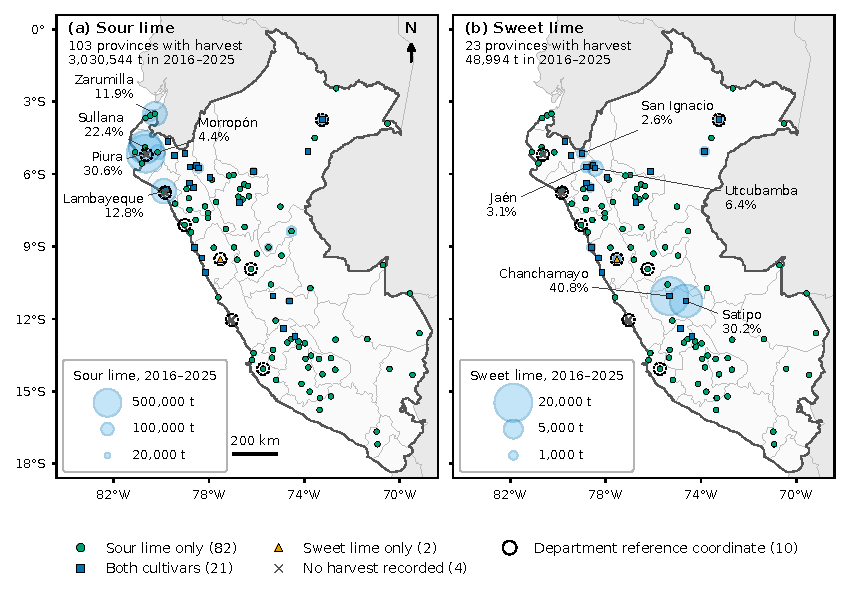
\includegraphics[width=\linewidth,height=0.8\textheight,keepaspectratio]{fig29_study_area_map.pdf}
\caption{\figcap{fig29_study_area_map}}
\label{fig:fig29_study_area_map}
\end{figure}

\begin{figure}[htbp]
\centering
\begin{subfigure}{\linewidth}
\centering
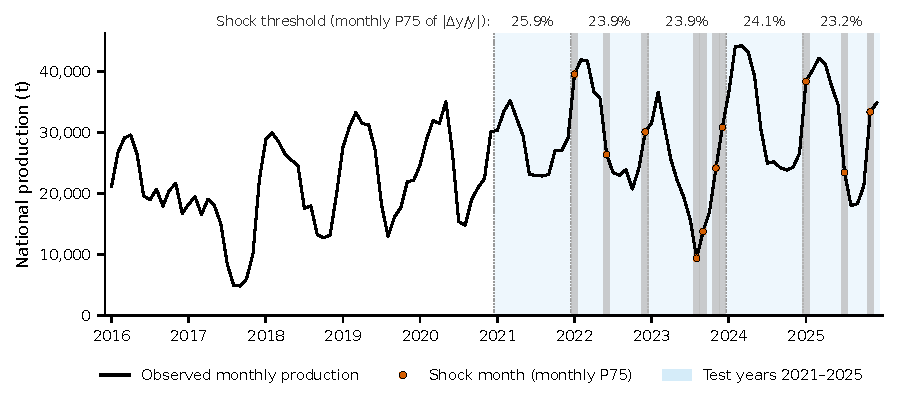
\includegraphics[width=\linewidth,height=0.36\textheight,keepaspectratio]{fig24_series_with_shocks_sutil.pdf}
\caption{Sour lime}
\label{fig:fig24_series_with_shocks_sutil}
\end{subfigure}
\par\medskip
\begin{subfigure}{\linewidth}
\centering
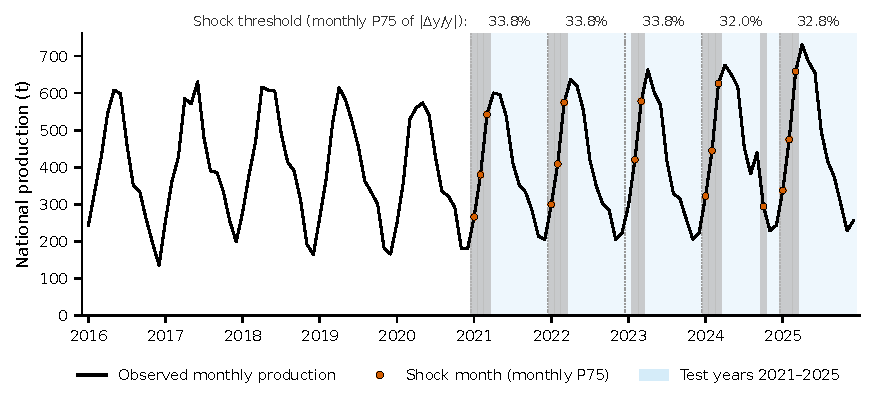
\includegraphics[width=\linewidth,height=0.36\textheight,keepaspectratio]{fig24_series_with_shocks_dulce.pdf}
\caption{Sweet lime}
\label{fig:fig24_series_with_shocks_dulce}
\end{subfigure}
\caption{\textit{Sour lime:} \figcap{fig24_series_with_shocks_sutil} \textit{Sweet lime:} \figcap{fig24_series_with_shocks_dulce}}
\label{fig:fig24_series_with_shocks}
\end{figure}

\begin{figure}[htbp]
\centering
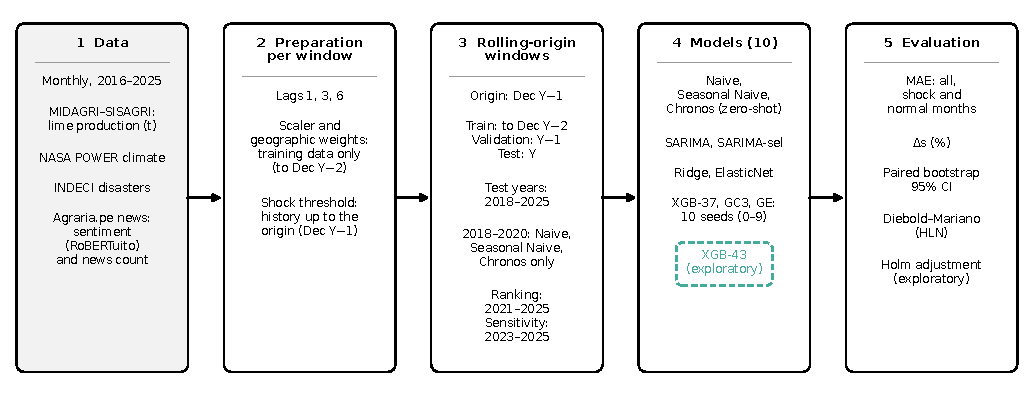
\includegraphics[width=\linewidth,height=0.8\textheight,keepaspectratio]{fig_workflow.pdf}
\caption{\figcap{fig_workflow}}
\label{fig:fig_workflow}
\end{figure}

\begin{figure}[htbp]
\centering
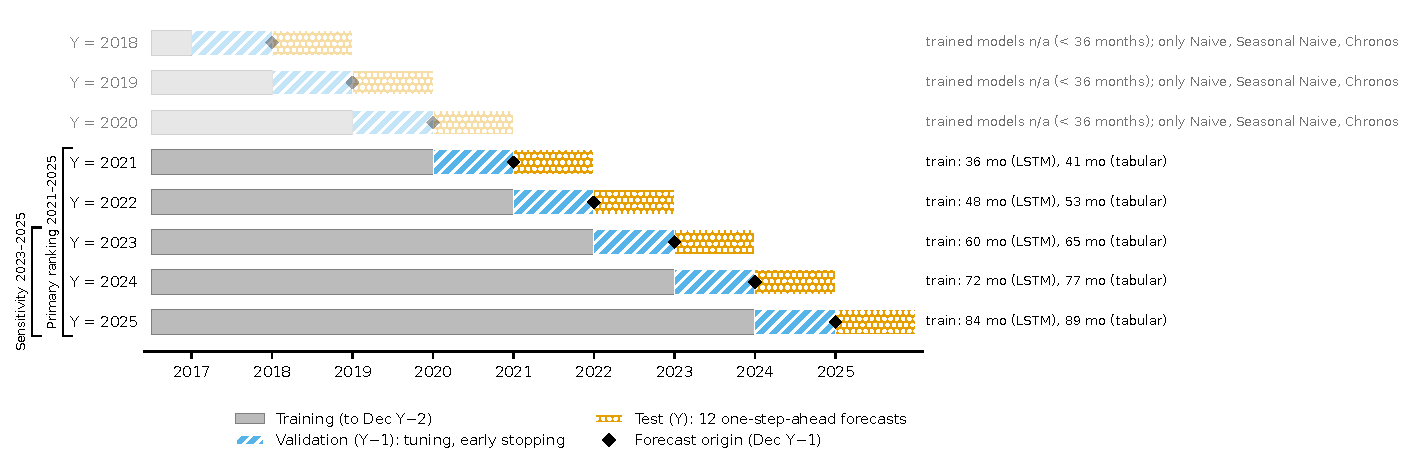
\includegraphics[width=\linewidth,height=0.8\textheight,keepaspectratio]{fig30_rolling_origin_scheme.pdf}
\caption{\figcap{fig30_rolling_origin_scheme}}
\label{fig:fig30_rolling_origin_scheme}
\end{figure}

\begin{figure}[htbp]
\centering
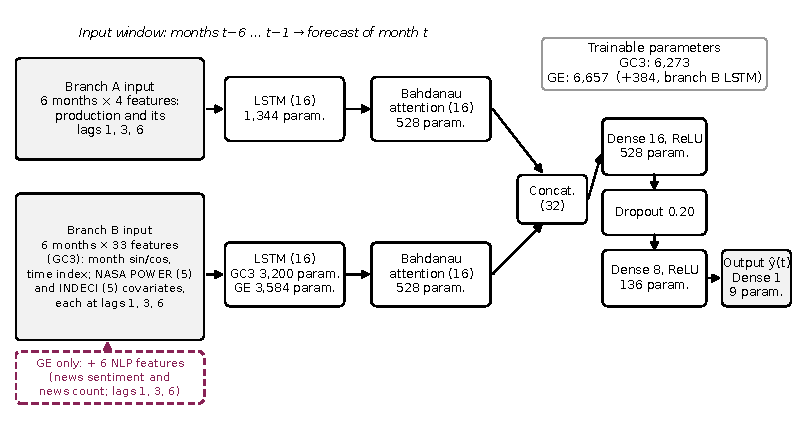
\includegraphics[width=\linewidth,height=0.8\textheight,keepaspectratio]{fig25_architecture_dual_lstm.pdf}
\caption{\figcap{fig25_architecture_dual_lstm}}
\label{fig:fig25_architecture_dual_lstm}
\end{figure}

\begin{figure}[htbp]
\centering
\begin{subfigure}{\linewidth}
\centering
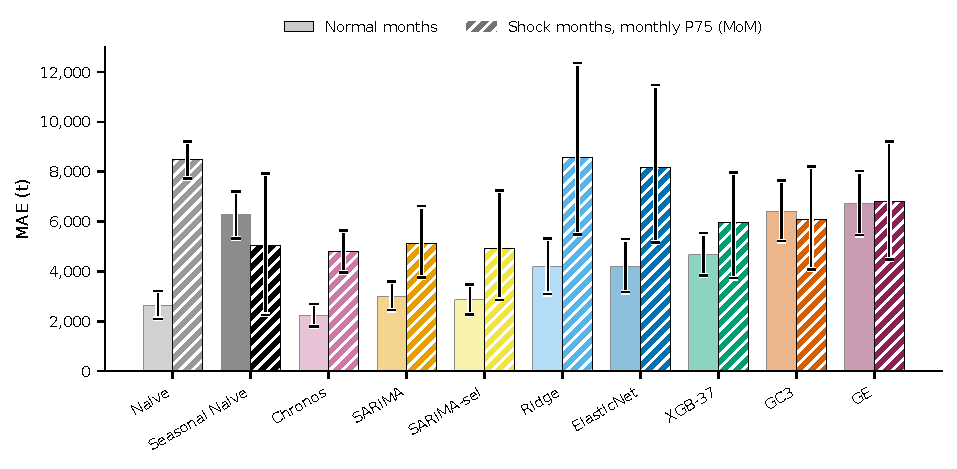
\includegraphics[width=\linewidth,height=0.36\textheight,keepaspectratio]{fig13_mae_normal_vs_shock_bars_sutil.pdf}
\caption{Sour lime}
\label{fig:fig13_mae_normal_vs_shock_bars_sutil}
\end{subfigure}
\par\medskip
\begin{subfigure}{\linewidth}
\centering
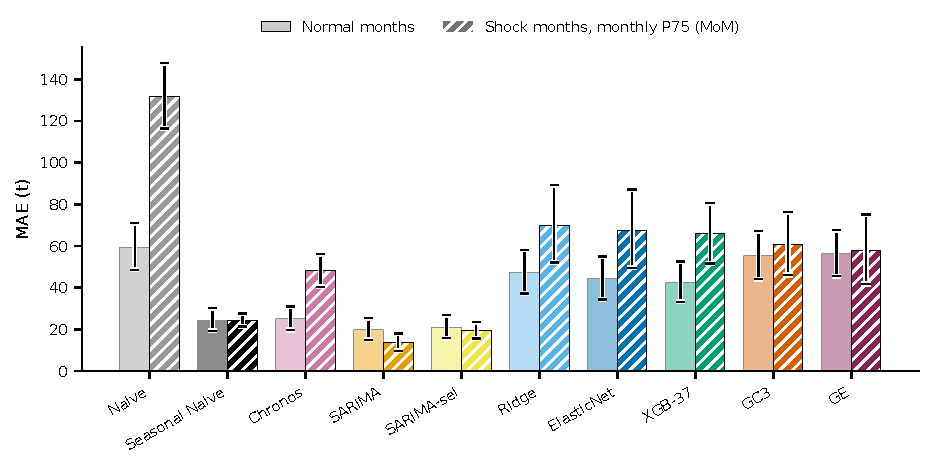
\includegraphics[width=\linewidth,height=0.36\textheight,keepaspectratio]{fig13_mae_normal_vs_shock_bars_dulce.pdf}
\caption{Sweet lime}
\label{fig:fig13_mae_normal_vs_shock_bars_dulce}
\end{subfigure}
\caption{\textit{Sour lime:} \figcap{fig13_mae_normal_vs_shock_bars_sutil} \textit{Sweet lime:} \figcap{fig13_mae_normal_vs_shock_bars_dulce}}
\label{fig:fig13_mae_normal_vs_shock_bars}
\end{figure}

\begin{figure}[htbp]
\centering
\begin{subfigure}{\linewidth}
\centering
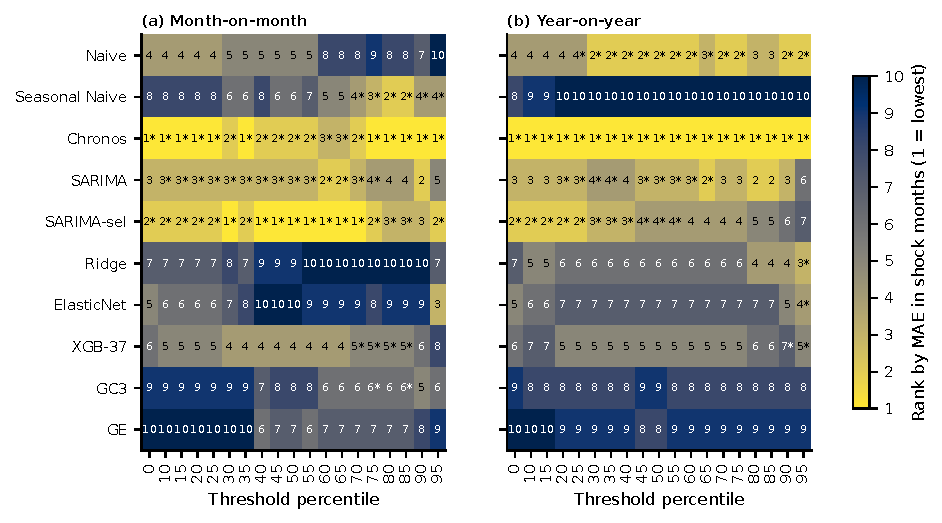
\includegraphics[width=\linewidth,height=0.36\textheight,keepaspectratio]{fig07_rank_heatmap_model_percentile_sutil.pdf}
\caption{Sour lime}
\label{fig:fig07_rank_heatmap_model_percentile_sutil}
\end{subfigure}
\par\medskip
\begin{subfigure}{\linewidth}
\centering
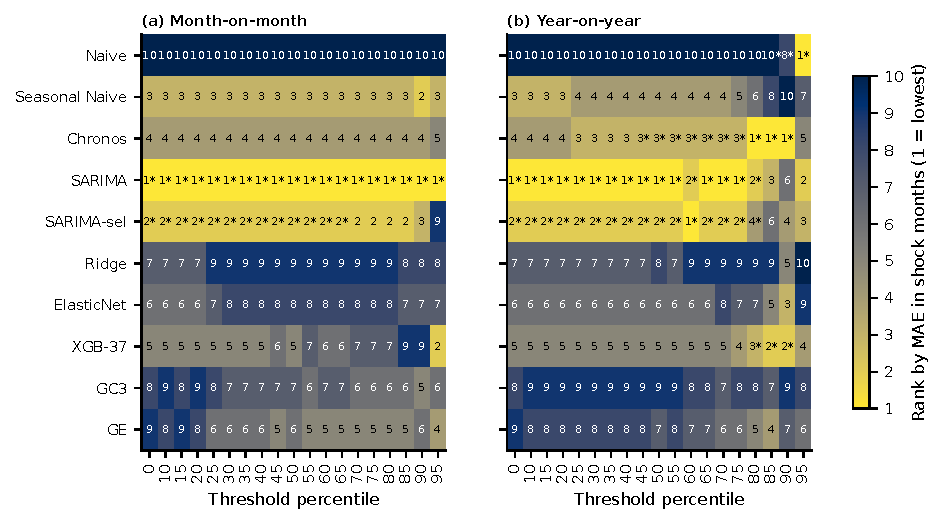
\includegraphics[width=\linewidth,height=0.36\textheight,keepaspectratio]{fig07_rank_heatmap_model_percentile_dulce.pdf}
\caption{Sweet lime}
\label{fig:fig07_rank_heatmap_model_percentile_dulce}
\end{subfigure}
\caption{\textit{Sour lime:} \figcap{fig07_rank_heatmap_model_percentile_sutil} \textit{Sweet lime:} \figcap{fig07_rank_heatmap_model_percentile_dulce}}
\label{fig:fig07_rank_heatmap_model_percentile}
\end{figure}

\begin{figure}[htbp]
\centering
\begin{subfigure}{\linewidth}
\centering
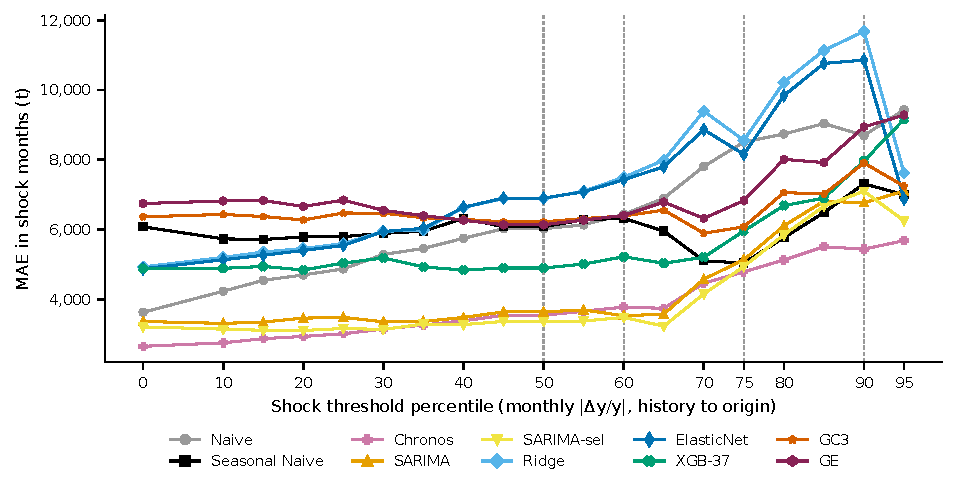
\includegraphics[width=\linewidth,height=0.36\textheight,keepaspectratio]{fig05_mae_shock_vs_percentile_sutil.pdf}
\caption{Sour lime}
\label{fig:fig05_mae_shock_vs_percentile_sutil}
\end{subfigure}
\par\medskip
\begin{subfigure}{\linewidth}
\centering
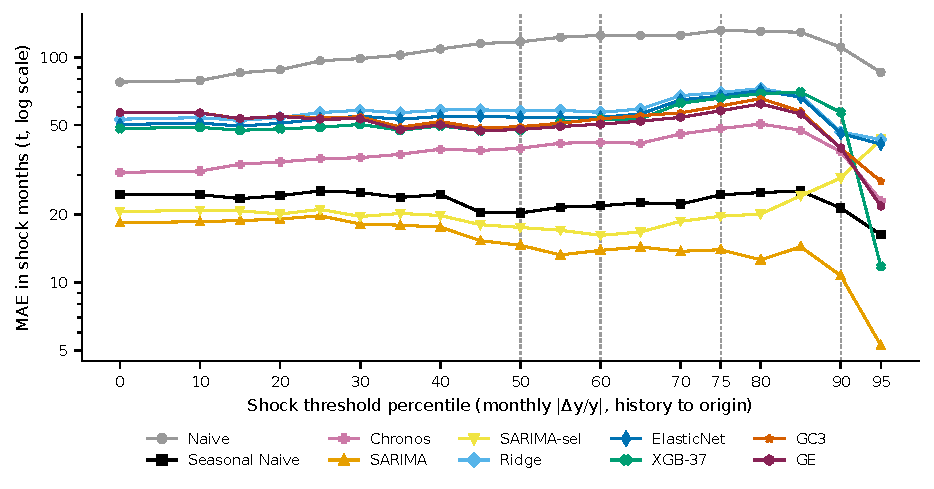
\includegraphics[width=\linewidth,height=0.36\textheight,keepaspectratio]{fig05_mae_shock_vs_percentile_dulce.pdf}
\caption{Sweet lime}
\label{fig:fig05_mae_shock_vs_percentile_dulce}
\end{subfigure}
\caption{\textit{Sour lime:} \figcap{fig05_mae_shock_vs_percentile_sutil} \textit{Sweet lime:} \figcap{fig05_mae_shock_vs_percentile_dulce}}
\label{fig:fig05_mae_shock_vs_percentile}
\end{figure}

\begin{figure}[htbp]
\centering
\begin{subfigure}{\linewidth}
\centering
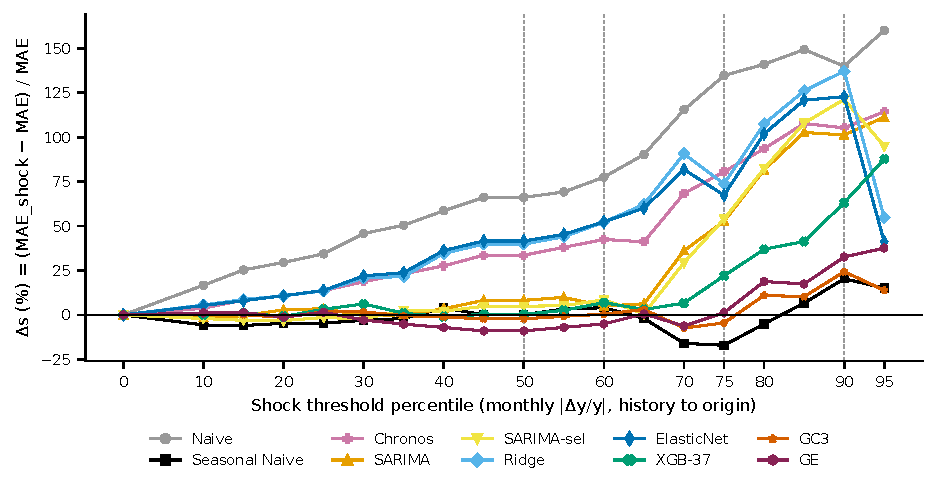
\includegraphics[width=\linewidth,height=0.36\textheight,keepaspectratio]{fig04_delta_s_vs_percentile_sutil.pdf}
\caption{Sour lime}
\label{fig:fig04_delta_s_vs_percentile_sutil}
\end{subfigure}
\par\medskip
\begin{subfigure}{\linewidth}
\centering
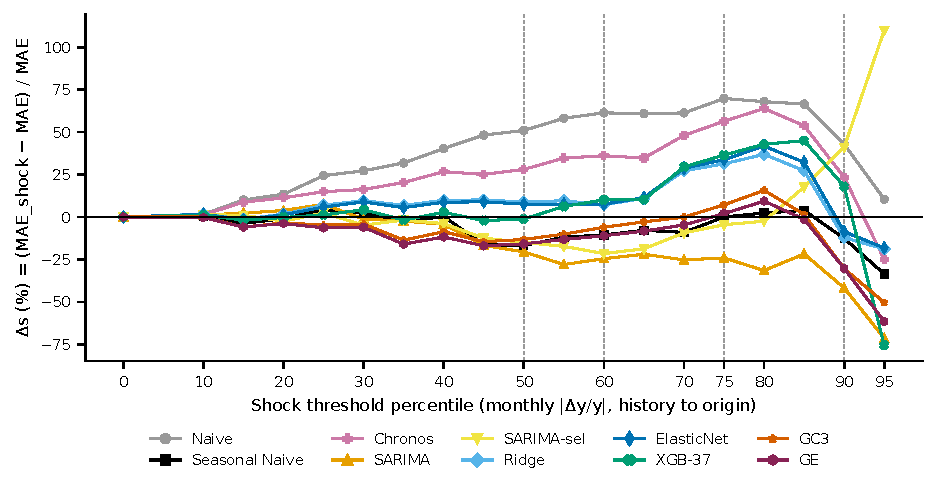
\includegraphics[width=\linewidth,height=0.36\textheight,keepaspectratio]{fig04_delta_s_vs_percentile_dulce.pdf}
\caption{Sweet lime}
\label{fig:fig04_delta_s_vs_percentile_dulce}
\end{subfigure}
\caption{\textit{Sour lime:} \figcap{fig04_delta_s_vs_percentile_sutil} \textit{Sweet lime:} \figcap{fig04_delta_s_vs_percentile_dulce}}
\label{fig:fig04_delta_s_vs_percentile}
\end{figure}

\begin{figure}[htbp]
\centering
\begin{subfigure}{\linewidth}
\centering
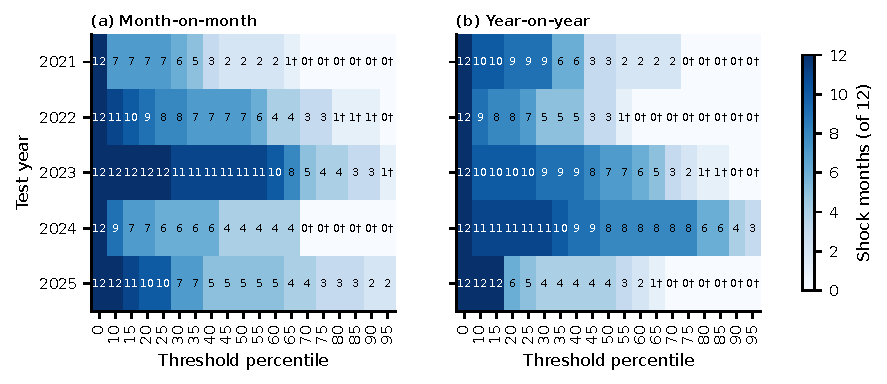
\includegraphics[width=\linewidth,height=0.36\textheight,keepaspectratio]{fig10_n_shock_heatmap_window_percentile_sutil.pdf}
\caption{Sour lime}
\label{fig:fig10_n_shock_heatmap_window_percentile_sutil}
\end{subfigure}
\par\medskip
\begin{subfigure}{\linewidth}
\centering
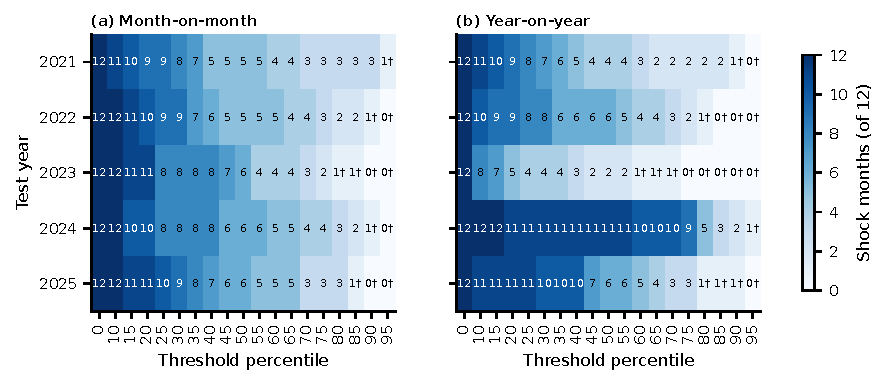
\includegraphics[width=\linewidth,height=0.36\textheight,keepaspectratio]{fig10_n_shock_heatmap_window_percentile_dulce.pdf}
\caption{Sweet lime}
\label{fig:fig10_n_shock_heatmap_window_percentile_dulce}
\end{subfigure}
\caption{\textit{Sour lime:} \figcap{fig10_n_shock_heatmap_window_percentile_sutil} \textit{Sweet lime:} \figcap{fig10_n_shock_heatmap_window_percentile_dulce}}
\label{fig:fig10_n_shock_heatmap_window_percentile}
\end{figure}

\begin{figure}[htbp]
\centering
\begin{subfigure}{\linewidth}
\centering
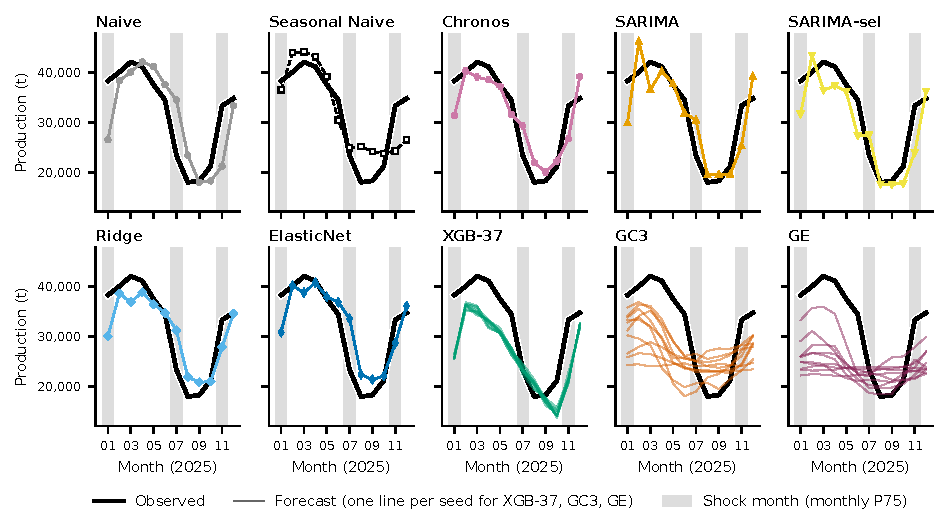
\includegraphics[width=\linewidth,height=0.36\textheight,keepaspectratio]{fig20_real_vs_pred_2025_sutil.pdf}
\caption{Sour lime}
\label{fig:fig20_real_vs_pred_2025_sutil}
\end{subfigure}
\par\medskip
\begin{subfigure}{\linewidth}
\centering
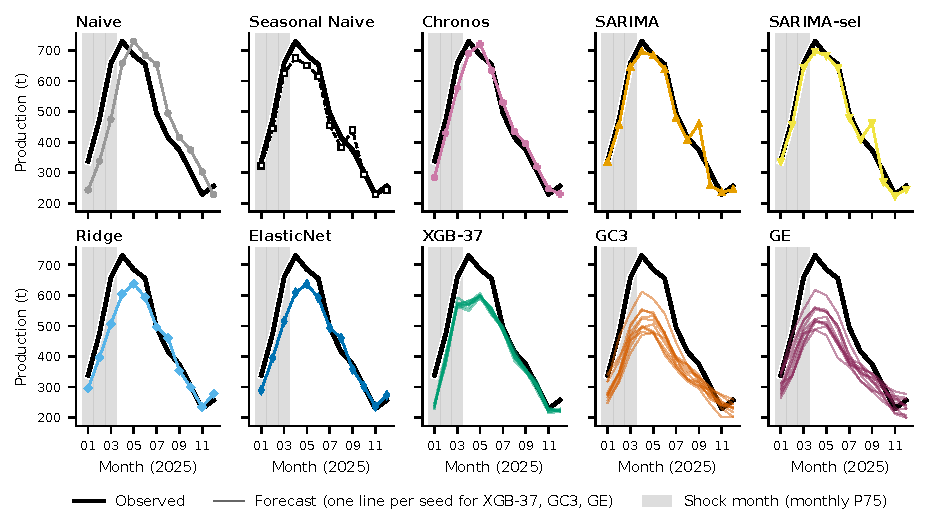
\includegraphics[width=\linewidth,height=0.36\textheight,keepaspectratio]{fig20_real_vs_pred_2025_dulce.pdf}
\caption{Sweet lime}
\label{fig:fig20_real_vs_pred_2025_dulce}
\end{subfigure}
\caption{\textit{Sour lime:} \figcap{fig20_real_vs_pred_2025_sutil} \textit{Sweet lime:} \figcap{fig20_real_vs_pred_2025_dulce}}
\label{fig:fig20_real_vs_pred_2025}
\end{figure}

\begin{figure}[htbp]
\centering
\begin{subfigure}{\linewidth}
\centering
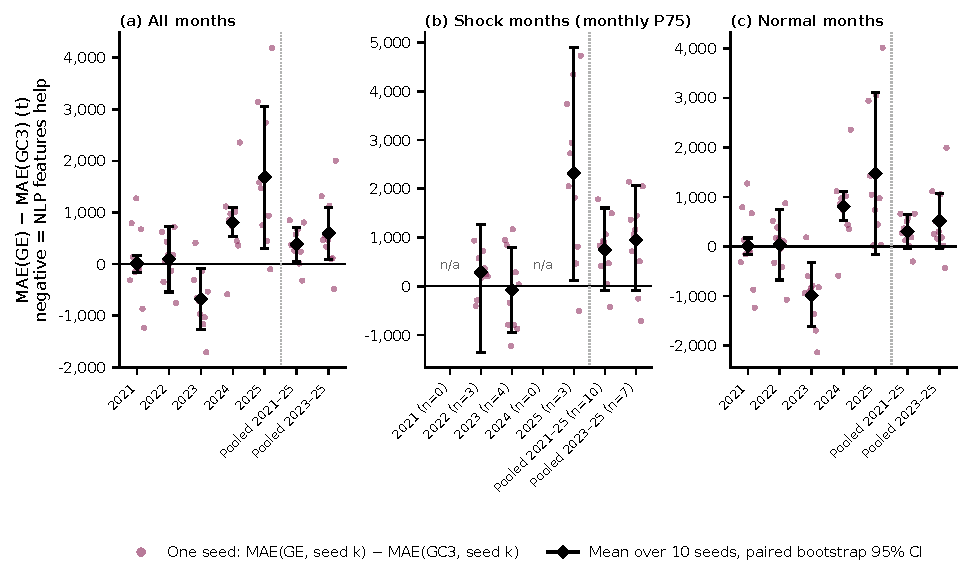
\includegraphics[width=\linewidth,height=0.36\textheight,keepaspectratio]{fig18_nlp_ablation_paired_sutil.pdf}
\caption{Sour lime}
\label{fig:fig18_nlp_ablation_paired_sutil}
\end{subfigure}
\par\medskip
\begin{subfigure}{\linewidth}
\centering
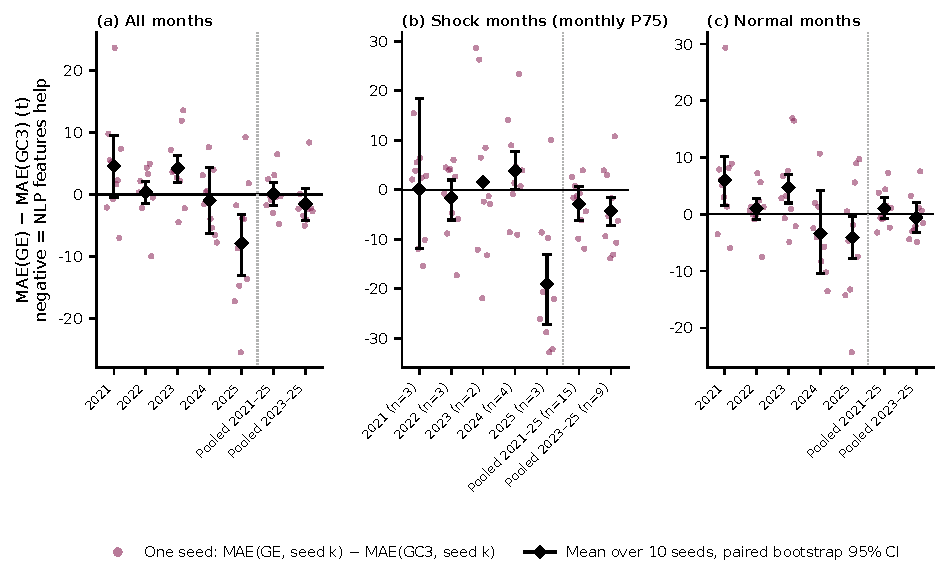
\includegraphics[width=\linewidth,height=0.36\textheight,keepaspectratio]{fig18_nlp_ablation_paired_dulce.pdf}
\caption{Sweet lime}
\label{fig:fig18_nlp_ablation_paired_dulce}
\end{subfigure}
\caption{\textit{Sour lime:} \figcap{fig18_nlp_ablation_paired_sutil} \textit{Sweet lime:} \figcap{fig18_nlp_ablation_paired_dulce}}
\label{fig:fig18_nlp_ablation_paired}
\end{figure}

\begin{figure}[htbp]
\centering
\begin{subfigure}{\linewidth}
\centering
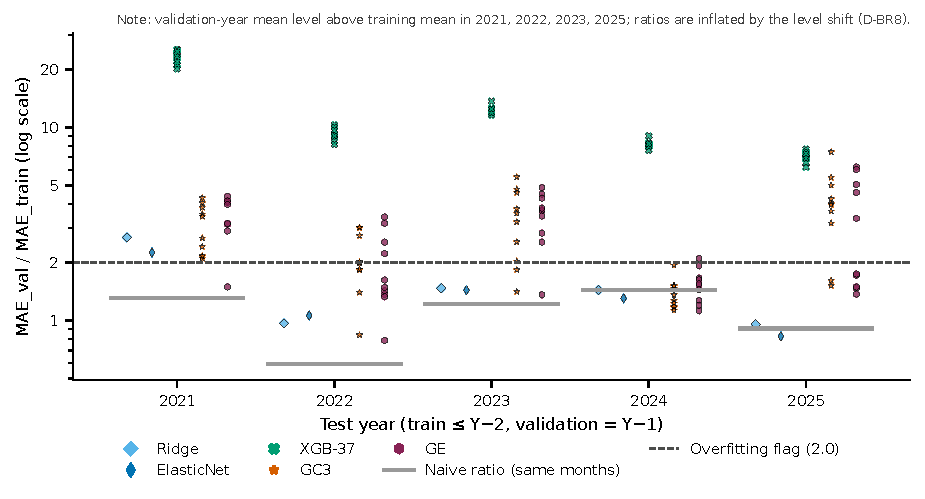
\includegraphics[width=\linewidth,height=0.36\textheight,keepaspectratio]{fig02_train_val_gap_sutil.pdf}
\caption{Sour lime}
\label{fig:fig02_train_val_gap_sutil}
\end{subfigure}
\par\medskip
\begin{subfigure}{\linewidth}
\centering
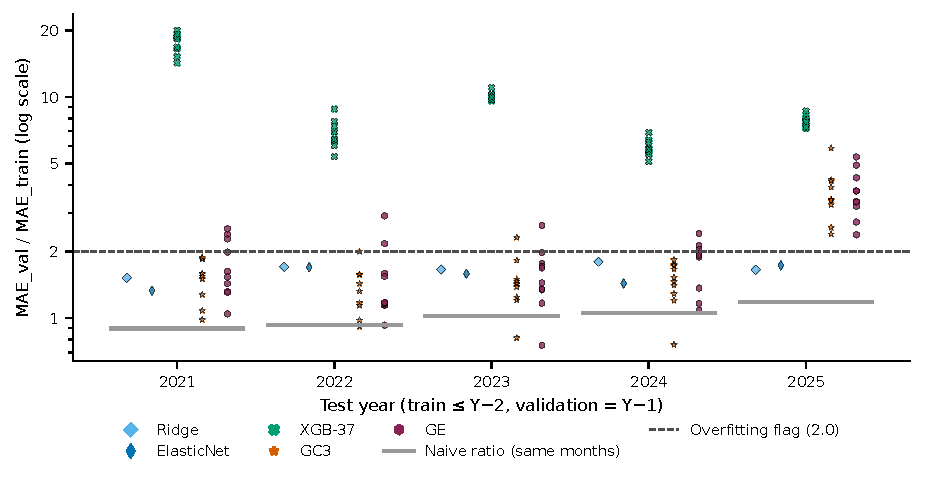
\includegraphics[width=\linewidth,height=0.36\textheight,keepaspectratio]{fig02_train_val_gap_dulce.pdf}
\caption{Sweet lime}
\label{fig:fig02_train_val_gap_dulce}
\end{subfigure}
\caption{\textit{Sour lime:} \figcap{fig02_train_val_gap_sutil} \textit{Sweet lime:} \figcap{fig02_train_val_gap_dulce}}
\label{fig:fig02_train_val_gap}
\end{figure}

% ===== SUPLEMENTARIO =====

% ===== tables_supp.tex =====
% Tables, supplementary material, in order of appearance.

\begin{landscape}
\scriptsize
\setlength{\tabcolsep}{3pt}
% --- tables/TS1_provinces.tex
\begin{longtable}{llrrllrrrrrr}
\caption{Lime-producing provinces of Peru, January 2016–December 2025 (MIDAGRI–SISAGRI (accessed \midagridate{})). Shares are relative to the national total of each cultivar; months with production count the months with production $>$ 0 out of 120.} \label{tab:S1_provinces} \\
\toprule
Department & Province & Latitude & Longitude & Coordinate & Category & Sour lime 2016-2025 (t) & Sour lime share (\%) & Months with sour lime $>$ 0 (of 120) & Sweet lime 2016-2025 (t) & Sweet lime share (\%) & Months with sweet lime $>$ 0 (of 120) \\
\midrule
\endfirsthead
\caption[]{Lime-producing provinces of Peru, January 2016–December 2025 (MIDAGRI–SISAGRI (accessed \midagridate{})). Shares are relative to the national total of each cultivar; months with production count the months with production $>$ 0 out of 120.} \\
\toprule
Department & Province & Latitude & Longitude & Coordinate & Category & Sour lime 2016-2025 (t) & Sour lime share (\%) & Months with sour lime $>$ 0 (of 120) & Sweet lime 2016-2025 (t) & Sweet lime share (\%) & Months with sweet lime $>$ 0 (of 120) \\
\midrule
\endhead
\midrule
\multicolumn{12}{r}{Continued on next page} \\
\midrule
\endfoot
\bottomrule
\endlastfoot
PIURA & PIURA & -5.15 & -80.66 & province & Sour lime only & 926,666.00 & 30.58 & 120.00 & 0.00 & 0.00 & 0.00 \\
PIURA & SULLANA & -4.89 & -80.69 & province & Sour lime only & 678,010.00 & 22.37 & 120.00 & 0.00 & 0.00 & 0.00 \\
LAMBAYEQUE & LAMBAYEQUE & -6.71 & -79.90 & province & Sour lime only & 386,555.00 & 12.76 & 120.00 & 0.00 & 0.00 & 0.00 \\
TUMBES & ZARUMILLA & -3.50 & -80.28 & province & Sour lime only & 361,442.10 & 11.93 & 120.00 & 0.00 & 0.00 & 0.00 \\
PIURA & MORROPON & -5.10 & -80.16 & province & Sour lime only & 132,988.00 & 4.39 & 120.00 & 0.00 & 0.00 & 0.00 \\
TUMBES & TUMBES & -3.57 & -80.46 & province & Sour lime only & 74,185.40 & 2.45 & 120.00 & 0.00 & 0.00 & 0.00 \\
UCAYALI & CORONEL PORTILLO & -8.37 & -74.54 & province & Sour lime only & 61,919.70 & 2.04 & 120.00 & 0.00 & 0.00 & 0.00 \\
LORETO & MAYNAS & -3.75 & -73.24 & province & Both cultivars & 55,277.00 & 1.82 & 120.00 & 942.00 & 1.92 & 40.00 \\
AMAZONAS & UTCUBAMBA & -5.75 & -78.44 & province & Both cultivars & 52,073.80 & 1.72 & 120.00 & 3,150.10 & 6.43 & 120.00 \\
UCAYALI & PADRE ABAD & -9.03 & -75.51 & province & Sour lime only & 32,399.90 & 1.07 & 120.00 & 0.00 & 0.00 & 0.00 \\
LORETO & ALTO AMAZONAS & -5.88 & -76.13 & province & Both cultivars & 26,941.00 & 0.89 & 120.00 & 67.00 & 0.14 & 39.00 \\
JUNIN & SATIPO & -11.25 & -74.64 & province & Both cultivars & 25,734.80 & 0.85 & 120.00 & 14,818.60 & 30.25 & 104.00 \\
TUMBES & CONTRALMIRANTE VILLAR & -3.68 & -80.67 & province & Sour lime only & 16,441.30 & 0.54 & 120.00 & 0.00 & 0.00 & 0.00 \\
CUSCO & LA CONVENCION & -12.86 & -72.69 & province & Sour lime only & 16,102.80 & 0.53 & 118.00 & 0.00 & 0.00 & 0.00 \\
UCAYALI & ATALAYA & -10.73 & -73.76 & province & Sour lime only & 16,010.20 & 0.53 & 120.00 & 0.00 & 0.00 & 0.00 \\
LORETO & UCAYALI & -7.35 & -75.01 & province & Sour lime only & 10,926.00 & 0.36 & 120.00 & 0.00 & 0.00 & 0.00 \\
SAN MARTIN & SAN MARTIN & -6.49 & -76.36 & province & Sour lime only & 9,544.10 & 0.31 & 120.00 & 0.00 & 0.00 & 0.00 \\
SAN MARTIN & PICOTA & -6.92 & -76.33 & province & Sour lime only & 8,634.60 & 0.28 & 120.00 & 0.00 & 0.00 & 0.00 \\
HUANUCO & LEONCIO PRADO & -9.30 & -76.00 & province & Sour lime only & 8,021.60 & 0.26 & 119.00 & 0.00 & 0.00 & 0.00 \\
SAN MARTIN & LAMAS & -6.42 & -76.52 & province & Sour lime only & 7,705.30 & 0.25 & 120.00 & 0.00 & 0.00 & 0.00 \\
JUNIN & CHANCHAMAYO & -11.06 & -75.33 & province & Both cultivars & 7,518.10 & 0.25 & 120.00 & 20,007.60 & 40.84 & 120.00 \\
ICA & ICA & -14.06 & -75.73 & province & Sour lime only & 6,788.40 & 0.22 & 74.00 & 0.00 & 0.00 & 0.00 \\
LORETO & LORETO & -4.50 & -73.57 & province & Sour lime only & 5,785.00 & 0.19 & 120.00 & 0.00 & 0.00 & 0.00 \\
SAN MARTIN & HUALLAGA & -6.94 & -76.77 & province & Sour lime only & 4,744.00 & 0.16 & 120.00 & 0.00 & 0.00 & 0.00 \\
LORETO & MARISCAL RAMON CASTILLA & -3.91 & -70.52 & province & Sour lime only & 4,463.00 & 0.15 & 110.00 & 0.00 & 0.00 & 0.00 \\
ANCASH & CASMA & -9.48 & -78.31 & province & Both cultivars & 4,240.00 & 0.14 & 120.00 & 358.00 & 0.73 & 74.00 \\
LORETO & REQUENA & -5.06 & -73.86 & province & Both cultivars & 3,935.00 & 0.13 & 120.00 & 1,094.00 & 2.23 & 120.00 \\
ICA & PISCO & -13.71 & -76.20 & province & Sour lime only & 3,862.80 & 0.13 & 54.00 & 0.00 & 0.00 & 0.00 \\
ICA & NASCA & -14.07 & -75.73 & department reference & Sour lime only & 3,794.00 & 0.13 & 31.00 & 0.00 & 0.00 & 0.00 \\
MADRE DE DIOS & TAMBOPATA & -12.59 & -69.18 & province & Sour lime only & 3,780.20 & 0.12 & 120.00 & 0.00 & 0.00 & 0.00 \\
SAN MARTIN & MARISCAL CACERES & -7.18 & -76.72 & province & Both cultivars & 3,678.70 & 0.12 & 111.00 & 199.80 & 0.41 & 84.00 \\
PIURA & AYABACA & -4.64 & -79.72 & province & Both cultivars & 3,610.90 & 0.12 & 113.00 & 1.00 & 0.00 & 1.00 \\
LORETO & DATEM DEL MARAÑON & -3.75 & -73.25 & department reference & Sour lime only & 3,254.00 & 0.11 & 110.00 & 0.00 & 0.00 & 0.00 \\
SAN MARTIN & BELLAVISTA & -7.05 & -76.59 & province & Sour lime only & 3,180.00 & 0.10 & 120.00 & 0.00 & 0.00 & 0.00 \\
SAN MARTIN & MOYOBAMBA & -6.03 & -76.97 & province & Sour lime only & 2,903.80 & 0.10 & 84.00 & 0.00 & 0.00 & 0.00 \\
SAN MARTIN & TOCACHE & -8.19 & -76.51 & province & Sour lime only & 2,898.80 & 0.10 & 109.00 & 0.00 & 0.00 & 0.00 \\
AMAZONAS & LUYA & -6.14 & -77.95 & province & Both cultivars & 2,812.70 & 0.09 & 120.00 & 330.90 & 0.68 & 120.00 \\
AMAZONAS & BAGUA & -5.64 & -78.53 & province & Both cultivars & 2,484.90 & 0.08 & 120.00 & 951.70 & 1.94 & 120.00 \\
AMAZONAS & CHACHAPOYAS & -6.23 & -77.87 & province & Sour lime only & 2,427.00 & 0.08 & 120.00 & 0.00 & 0.00 & 0.00 \\
SAN MARTIN & RIOJA & -6.06 & -77.17 & province & Sour lime only & 2,318.80 & 0.08 & 109.00 & 0.00 & 0.00 & 0.00 \\
PIURA & HUANCABAMBA & -5.24 & -79.45 & province & Both cultivars & 2,031.20 & 0.07 & 118.00 & 30.20 & 0.06 & 9.00 \\
UCAYALI & PURUS & -9.77 & -70.71 & province & Sour lime only & 2,029.80 & 0.07 & 120.00 & 0.00 & 0.00 & 0.00 \\
CAJAMARCA & SAN MIGUEL & -7.00 & -78.85 & province & Sour lime only & 1,909.70 & 0.06 & 77.00 & 0.00 & 0.00 & 0.00 \\
SAN MARTIN & EL DORADO & -6.61 & -76.70 & province & Sour lime only & 1,855.70 & 0.06 & 114.00 & 0.00 & 0.00 & 0.00 \\
LA LIBERTAD & VIRU & -8.41 & -78.75 & province & Sour lime only & 1,720.90 & 0.06 & 120.00 & 0.00 & 0.00 & 0.00 \\
ANCASH & HUAYLAS & -9.05 & -77.80 & province & Sour lime only & 1,701.00 & 0.06 & 120.00 & 0.00 & 0.00 & 0.00 \\
CAJAMARCA & CHOTA & -6.56 & -78.65 & province & Both cultivars & 1,634.00 & 0.05 & 92.00 & 956.00 & 1.95 & 77.00 \\
HUANUCO & HUAMALIES & -9.55 & -76.82 & province & Sour lime only & 1,543.50 & 0.05 & 118.00 & 0.00 & 0.00 & 0.00 \\
PIURA & PAITA & -5.09 & -81.10 & province & Sour lime only & 1,444.00 & 0.05 & 110.00 & 0.00 & 0.00 & 0.00 \\
MADRE DE DIOS & MANU & -12.84 & -71.37 & province & Sour lime only & 1,404.00 & 0.05 & 120.00 & 0.00 & 0.00 & 0.00 \\
LORETO & PUTUMAYO & -2.45 & -72.67 & province & Sour lime only & 1,398.00 & 0.05 & 120.00 & 0.00 & 0.00 & 0.00 \\
LAMBAYEQUE & FERREÑAFE & -6.64 & -79.79 & province & Both cultivars & 1,376.80 & 0.05 & 54.00 & 71.00 & 0.14 & 10.00 \\
APURIMAC & ABANCAY & -13.63 & -72.89 & province & Sour lime only & 1,375.00 & 0.05 & 113.00 & 0.00 & 0.00 & 0.00 \\
CAJAMARCA & JAEN & -5.71 & -78.81 & province & Both cultivars & 1,253.30 & 0.04 & 120.00 & 1,528.10 & 3.12 & 96.00 \\
MADRE DE DIOS & TAHUAMANU & -10.95 & -69.58 & province & Sour lime only & 1,240.40 & 0.04 & 120.00 & 0.00 & 0.00 & 0.00 \\
JUNIN & HUANCAYO & -12.07 & -75.21 & province & Sour lime only & 1,196.70 & 0.04 & 120.00 & 0.00 & 0.00 & 0.00 \\
AYACUCHO & LA MAR & -13.01 & -73.98 & province & Sour lime only & 1,176.80 & 0.04 & 113.00 & 0.00 & 0.00 & 0.00 \\
PASCO & OXAPAMPA & -10.57 & -75.40 & province & Sour lime only & 1,030.30 & 0.03 & 28.00 & 0.00 & 0.00 & 0.00 \\
HUANCAVELICA & TAYACAJA & -12.40 & -74.87 & province & Both cultivars & 952.10 & 0.03 & 52.00 & 170.70 & 0.35 & 27.00 \\
LA LIBERTAD & BOLIVAR & -7.15 & -77.70 & province & Sour lime only & 799.80 & 0.03 & 104.00 & 0.00 & 0.00 & 0.00 \\
APURIMAC & CHINCHEROS & -13.52 & -73.72 & province & Sour lime only & 787.40 & 0.03 & 43.00 & 0.00 & 0.00 & 0.00 \\
APURIMAC & ANDAHUAYLAS & -13.66 & -73.39 & province & Sour lime only & 751.40 & 0.02 & 46.00 & 0.00 & 0.00 & 0.00 \\
HUANUCO & HUANUCO & -9.93 & -76.24 & province & Sour lime only & 676.60 & 0.02 & 115.00 & 0.00 & 0.00 & 0.00 \\
LA LIBERTAD & PATAZ & -8.28 & -77.30 & province & Sour lime only & 664.10 & 0.02 & 91.00 & 0.00 & 0.00 & 0.00 \\
CAJAMARCA & CAJABAMBA & -7.62 & -78.05 & province & Sour lime only & 661.90 & 0.02 & 118.00 & 0.00 & 0.00 & 0.00 \\
AYACUCHO & HUANTA & -12.94 & -74.25 & province & Sour lime only & 656.50 & 0.02 & 83.00 & 0.00 & 0.00 & 0.00 \\
ANCASH & SANTA & -9.04 & -78.61 & province & Both cultivars & 634.00 & 0.02 & 119.00 & 910.00 & 1.86 & 112.00 \\
ANCASH & HUARMEY & -10.07 & -78.15 & province & Both cultivars & 537.00 & 0.02 & 115.00 & 301.00 & 0.61 & 72.00 \\
AYACUCHO & LUCANAS & -14.69 & -74.12 & province & Sour lime only & 534.00 & 0.02 & 54.00 & 0.00 & 0.00 & 0.00 \\
HUANUCO & PUERTO INCA & -9.38 & -74.97 & province & Sour lime only & 520.60 & 0.02 & 110.00 & 0.00 & 0.00 & 0.00 \\
HUANUCO & HUACAYBAMBA & -9.04 & -76.95 & province & Sour lime only & 507.20 & 0.02 & 46.00 & 0.00 & 0.00 & 0.00 \\
LA LIBERTAD & CHEPEN & -7.23 & -79.43 & province & Sour lime only & 499.50 & 0.02 & 67.00 & 0.00 & 0.00 & 0.00 \\
AYACUCHO & PAUCAR DEL SARA SARA & -15.28 & -73.34 & province & Sour lime only & 496.00 & 0.02 & 44.00 & 0.00 & 0.00 & 0.00 \\
AYACUCHO & VILCAS HUAMAN & -13.65 & -73.95 & province & Sour lime only & 479.60 & 0.02 & 69.00 & 0.00 & 0.00 & 0.00 \\
LA LIBERTAD & SANCHEZ CARRION & -7.81 & -78.05 & province & Sour lime only & 465.80 & 0.02 & 108.00 & 0.00 & 0.00 & 0.00 \\
PIURA & SECHURA & -5.56 & -80.82 & province & Sour lime only & 464.00 & 0.02 & 109.00 & 0.00 & 0.00 & 0.00 \\
PUNO & SANDIA & -14.32 & -69.47 & province & Sour lime only & 459.70 & 0.02 & 51.00 & 0.00 & 0.00 & 0.00 \\
HUANUCO & MARAÑON & -9.93 & -76.24 & department reference & Sour lime only & 458.50 & 0.02 & 80.00 & 0.00 & 0.00 & 0.00 \\
CAJAMARCA & SAN IGNACIO & -5.15 & -79.00 & province & Both cultivars & 425.70 & 0.01 & 76.00 & 1,274.50 & 2.60 & 84.00 \\
MOQUEGUA & GENERAL SANCHEZ CERRO & -16.67 & -70.97 & province & Sour lime only & 394.40 & 0.01 & 37.00 & 0.00 & 0.00 & 0.00 \\
MOQUEGUA & MARISCAL NIETO & -17.19 & -70.93 & province & Sour lime only & 359.70 & 0.01 & 35.00 & 0.00 & 0.00 & 0.00 \\
HUANCAVELICA & CHURCAMPA & -12.74 & -74.39 & province & Both cultivars & 336.40 & 0.01 & 60.00 & 141.90 & 0.29 & 49.00 \\
CAJAMARCA & SAN MARCOS & -7.34 & -78.17 & province & Sour lime only & 324.90 & 0.01 & 108.00 & 0.00 & 0.00 & 0.00 \\
LIMA & HUAURA & -11.11 & -77.61 & province & Sour lime only & 308.90 & 0.01 & 20.00 & 0.00 & 0.00 & 0.00 \\
CAJAMARCA & SANTA CRUZ & -6.63 & -78.94 & province & Sour lime only & 305.00 & 0.01 & 50.00 & 0.00 & 0.00 & 0.00 \\
AREQUIPA & LA UNION & -15.21 & -72.89 & province & Sour lime only & 281.30 & 0.01 & 10.00 & 0.00 & 0.00 & 0.00 \\
ICA & PALPA & -14.53 & -75.19 & province & Sour lime only & 258.90 & 0.01 & 25.00 & 0.00 & 0.00 & 0.00 \\
HUANCAVELICA & ACOBAMBA & -12.84 & -74.57 & province & Sour lime only & 229.60 & 0.01 & 51.00 & 0.00 & 0.00 & 0.00 \\
APURIMAC & AYMARAES & -14.29 & -73.24 & province & Sour lime only & 189.50 & 0.01 & 117.00 & 0.00 & 0.00 & 0.00 \\
AYACUCHO & SUCRE & -14.01 & -73.84 & province & Sour lime only & 177.00 & 0.01 & 22.00 & 0.00 & 0.00 & 0.00 \\
AYACUCHO & HUAMANGA & -13.16 & -74.23 & province & Sour lime only & 175.20 & 0.01 & 118.00 & 0.00 & 0.00 & 0.00 \\
AREQUIPA & CARAVELI & -15.77 & -73.37 & province & Sour lime only & 165.90 & 0.01 & 17.00 & 0.00 & 0.00 & 0.00 \\
HUANCAVELICA & ANGARAES & -12.98 & -74.72 & province & Sour lime only & 158.90 & 0.01 & 50.00 & 0.00 & 0.00 & 0.00 \\
HUANCAVELICA & HUAYTARA & -13.60 & -75.35 & province & Sour lime only & 150.90 & 0.00 & 66.00 & 0.00 & 0.00 & 0.00 \\
LA LIBERTAD & GRAN CHIMU & -7.48 & -78.82 & province & Sour lime only & 143.90 & 0.00 & 70.00 & 0.00 & 0.00 & 0.00 \\
AYACUCHO & PARINACOCHAS & -15.02 & -73.78 & province & Sour lime only & 131.00 & 0.00 & 40.00 & 0.00 & 0.00 & 0.00 \\
HUANCAVELICA & CASTROVIRREYNA & -13.28 & -75.32 & province & Sour lime only & 127.70 & 0.00 & 79.00 & 0.00 & 0.00 & 0.00 \\
LA LIBERTAD & ASCOPE & -8.11 & -79.03 & department reference & Sour lime only & 121.70 & 0.00 & 52.00 & 0.00 & 0.00 & 0.00 \\
PUNO & CARABAYA & -14.07 & -70.43 & province & Sour lime only & 107.00 & 0.00 & 40.00 & 0.00 & 0.00 & 0.00 \\
LA LIBERTAD & OTUZCO & -7.90 & -78.57 & province & Sour lime only & 106.90 & 0.00 & 73.00 & 0.00 & 0.00 & 0.00 \\
APURIMAC & GRAU & -14.11 & -72.71 & province & Sour lime only & 80.00 & 0.00 & 51.00 & 0.00 & 0.00 & 0.00 \\
ICA & CHINCHA & -13.42 & -76.13 & province & Sour lime only & 76.40 & 0.00 & 13.00 & 0.00 & 0.00 & 0.00 \\
CAJAMARCA & CUTERVO & -6.38 & -78.82 & province & Both cultivars & 21.00 & 0.00 & 4.00 & 309.00 & 0.63 & 37.00 \\
ANCASH & CARHUAZ & -9.53 & -77.53 & department reference & Sweet lime only & 0.00 & 0.00 & 0.00 & 753.00 & 1.54 & 117.00 \\
ANCASH & YUNGAY & -9.53 & -77.53 & department reference & Sweet lime only & 0.00 & 0.00 & 0.00 & 628.00 & 1.28 & 119.00 \\
LAMBAYEQUE & CHICLAYO & -6.77 & -79.84 & department reference & No harvest recorded & 0.00 & 0.00 & 0.00 & 0.00 & 0.00 & 0.00 \\
LIMA & CAÑETE & -12.05 & -77.04 & department reference & No harvest recorded & 0.00 & 0.00 & 0.00 & 0.00 & 0.00 & 0.00 \\
LIMA & LIMA & -12.05 & -77.04 & department reference & No harvest recorded & 0.00 & 0.00 & 0.00 & 0.00 & 0.00 & 0.00 \\
PIURA & TALARA & -5.19 & -80.63 & department reference & No harvest recorded & 0.00 & 0.00 & 0.00 & 0.00 & 0.00 & 0.00 \\
TOTAL &  &  &  &  &  & 3,030,543.60 & 100.00 &  & 48,994.10 & 100.00 &  \\
\end{longtable}
\end{landscape}

% --- tables/T16_exploratorio_xgb43.tex
\begin{table}[H]
\centering
\small
\caption{EXPLORATORY (post-hoc): XGB-43 versus XGB-37, 2021-2025, monthly P75 (t)}
\label{tab:T16_exploratorio_xgb43}
\begin{tabular}{llllllll}
\toprule
Cultivar & Scope & Months & MAE XGB-37 & MAE XGB-43 & XGB-43 $-$ XGB-37 & 95\% CI lower & 95\% CI upper \\
\midrule
sutil & global & 60 & 4,881.4 & 5,011.9 & 130.5 & 1.5 & 260.4 \\
sutil & shock\_P75 & 10 & 5,955.2 & 5,997.2 & 42.0 & -240.1 & 338.3 \\
sutil & normal\_P75 & 50 & 4,666.7 & 4,814.9 & 148.2 & 6.5 & 286.3 \\
dulce & global & 60 & 48.3 & 47.6 & -0.6 & -2.4 & 1.2 \\
dulce & shock\_P75 & 15 & 65.8 & 62.2 & -3.6 & -5.9 & -1.2 \\
dulce & normal\_P75 & 45 & 42.4 & 42.8 & 0.4 & -1.7 & 2.5 \\
\bottomrule
\end{tabular}
\end{table}

% --- tables/T05_MAE_P75_por_ventana_sutil.tex
\begin{table}[H]
\centering
\small
\caption{MAE por ventana, P75 mensual, Sutil (t)}
\label{tab:T05_MAE_P75_por_ventana_sutil}
\begin{tabular}{llllll}
\toprule
modelo & 2021 & 2022 & 2023 & 2024 & 2025 \\
\midrule
Naive & 1,986 & 3,762 & 4,590 & 3,078 & 4,704 \\
Seasonal Naive & 4,590 & 4,136 & 7,638 & 9,850 & 4,160 \\
Chronos & 2,541 & 2,205 & 3,157 & 2,023 & 3,316 \\
SARIMA & 3,208 & 3,061 & 3,693 & 2,858 & 3,985 \\
SARIMA-sel & 2,304 & 2,609 & 3,836 & 3,333 & 3,947 \\
Ridge & 3,108 & 3,187 & 10,778 & 4,322 & 3,232 \\
ElasticNet & 3,006 & 2,968 & 10,413 & 4,751 & 3,223 \\
XGB-37 & 5,211 & 4,552 & 3,785 & 4,957 & 5,902 \\
GC3 & 3,856 & 5,162 & 6,074 & 8,969 & 7,746 \\
GE & 3,867 & 5,260 & 5,391 & 9,774 & 9,426 \\
XGB-43 & 5,333 & 4,664 & 3,679 & 5,466 & 5,918 \\
\bottomrule
\end{tabular}
\end{table}

% --- tables/T05_MAE_P75_por_ventana_dulce.tex
\begin{table}[H]
\centering
\small
\caption{MAE por ventana, P75 mensual, Dulce (t)}
\label{tab:T05_MAE_P75_por_ventana_dulce}
\begin{tabular}{llllll}
\toprule
modelo & 2021 & 2022 & 2023 & 2024 & 2025 \\
\midrule
Naive & 67.8 & 73.3 & 76.2 & 85.6 & 84.7 \\
Seasonal Naive & 18.4 & 19.9 & 11.8 & 41.8 & 30.5 \\
Chronos & 19.2 & 30.0 & 30.4 & 39.9 & 34.6 \\
SARIMA & 13.7 & 12.4 & 18.8 & 25.5 & 21.8 \\
SARIMA-sel & 27.9 & 12.4 & 17.4 & 25.6 & 19.8 \\
Ridge & 37.9 & 35.5 & 43.6 & 97.7 & 50.6 \\
ElasticNet & 37.6 & 35.2 & 43.4 & 85.7 & 49.3 \\
XGB-37 & 25.7 & 52.3 & 45.8 & 58.0 & 59.4 \\
GC3 & 36.5 & 37.2 & 38.0 & 68.2 & 103.4 \\
GE & 41.1 & 37.5 & 42.2 & 67.3 & 95.6 \\
XGB-43 & 26.2 & 52.2 & 44.3 & 54.1 & 61.4 \\
\bottomrule
\end{tabular}
\end{table}

% --- tables/T05_MAE_shock_P75_por_ventana_sutil.tex
\begin{table}[H]
\centering
\small
\caption{MAE\_shock por ventana, P75 mensual, Sutil (t)}
\label{tab:T05_MAE_shock_P75_por_ventana_sutil}
\begin{tabular}{llllll}
\toprule
modelo & 2021 (n=0) & 2022 (n=3) & 2023 (n=4) & 2024 (n=0) & 2025 (n=3) \\
\midrule
Naive & -- & 8,522 & 6,129 & -- & 11,660 \\
Seasonal Naive & -- & 4,472 & 6,135 & -- & 4,130 \\
Chronos & -- & 4,852 & 3,454 & -- & 6,487 \\
SARIMA & -- & 3,905 & 4,030 & -- & 7,824 \\
SARIMA-sel & -- & 4,207 & 4,158 & -- & 6,701 \\
Ridge & -- & 4,394 & 12,714 & -- & 7,177 \\
ElasticNet & -- & 4,015 & 11,806 & -- & 7,423 \\
XGB-37 & -- & 5,234 & 4,740 & -- & 8,297 \\
GC3 & -- & 4,916 & 7,304 & -- & 5,594 \\
GE & -- & 5,202 & 7,234 & -- & 7,908 \\
XGB-43 & -- & 5,374 & 4,656 & -- & 8,408 \\
\bottomrule
\end{tabular}
\end{table}

% --- tables/T05_MAE_shock_P75_por_ventana_dulce.tex
\begin{table}[H]
\centering
\small
\caption{MAE\_shock por ventana, P75 mensual, Dulce (t)}
\label{tab:T05_MAE_shock_P75_por_ventana_dulce}
\begin{tabular}{llllll}
\toprule
modelo & 2021 (n=3) & 2022 (n=3) & 2023 (n=2) & 2024 (n=4) & 2025 (n=3) \\
\midrule
Naive & 120.6 & 123.0 & 140.7 & 136.8 & 138.3 \\
Seasonal Naive & 16.0 & 31.5 & 7.4 & 33.2 & 25.9 \\
Chronos & 26.1 & 48.9 & 43.8 & 57.5 & 60.1 \\
SARIMA & 4.3 & 12.9 & 8.8 & 26.4 & 11.6 \\
SARIMA-sel & 34.9 & 12.9 & 7.5 & 25.9 & 11.0 \\
Ridge & 41.9 & 54.1 & 29.3 & 106.5 & 90.9 \\
ElasticNet & 43.5 & 53.5 & 29.7 & 96.5 & 90.7 \\
XGB-37 & 42.2 & 79.6 & 72.2 & 51.9 & 90.1 \\
GC3 & 43.7 & 44.3 & 50.9 & 47.1 & 118.9 \\
GE & 43.8 & 42.7 & 52.5 & 51.0 & 99.9 \\
XGB-43 & 40.0 & 78.9 & 73.3 & 45.9 & 82.3 \\
\bottomrule
\end{tabular}
\end{table}

% --- tables/T09_DM_matriz_principal_2021_2025_sutil.tex
\begin{table}[H]
\centering
\small
\caption{DM-HLN, p-valor sin ajustar (principal\_2021\_2025, Sutil). Bajo la diagonal: global (n=60); sobre la diagonal: solo shocks P75 mensual (n=10). Signo: + = el modelo de la fila tiene más error que el de la columna}
\label{tab:T09_DM_matriz_principal_2021_2025_sutil}
\begin{tabular}{lllllllllll}
\toprule
modelo & Nv & SN & Chr & SAR & SSel & Rdg & EN & X37 & GC3 & GE \\
\midrule
Naive & -- & 0.094+ & 0.000+ & 0.001+ & 0.013+ & 0.984- & 0.881+ & 0.045+ & 0.123+ & 0.259+ \\
Seasonal Naive & 0.001+ & -- & 0.867+ & 0.949- & 0.932+ & 0.235- & 0.247- & 0.614- & 0.331- & 0.245- \\
Chronos & 0.003- & 0.000- & -- & 0.509- & 0.867- & 0.145- & 0.146- & 0.292- & 0.255- & 0.109- \\
SARIMA & 0.548- & 0.000- & 0.017+ & -- & 0.807+ & 0.152- & 0.151- & 0.460- & 0.427- & 0.176- \\
SARIMA-sel & 0.385- & 0.000- & 0.102+ & 0.587- & -- & 0.156- & 0.157- & 0.358- & 0.243- & 0.090- \\
Ridge & 0.071+ & 0.180- & 0.002+ & 0.030+ & 0.022+ & -- & 0.406+ & 0.333+ & 0.344+ & 0.525+ \\
ElasticNet & 0.066+ & 0.129- & 0.002+ & 0.028+ & 0.018+ & 0.696- & -- & 0.389+ & 0.382+ & 0.598+ \\
XGB-37 & 0.018+ & 0.063- & 0.000+ & 0.004+ & 0.001+ & 0.955- & 0.990+ & -- & 0.919- & 0.301- \\
GC3 & 0.000+ & 0.641+ & 0.000+ & 0.000+ & 0.000+ & 0.080+ & 0.050+ & 0.001+ & -- & 0.225- \\
GE & 0.000+ & 0.341+ & 0.000+ & 0.000+ & 0.000+ & 0.045+ & 0.030+ & 0.000+ & 0.061+ & -- \\
\bottomrule
\end{tabular}
\end{table}

% --- tables/T09_DM_matriz_principal_2021_2025_dulce.tex
\begin{table}[H]
\centering
\small
\caption{DM-HLN, p-valor sin ajustar (principal\_2021\_2025, Dulce). Bajo la diagonal: global (n=60); sobre la diagonal: solo shocks P75 mensual (n=15). Signo: + = el modelo de la fila tiene más error que el de la columna}
\label{tab:T09_DM_matriz_principal_2021_2025_dulce}
\begin{tabular}{lllllllllll}
\toprule
modelo & Nv & SN & Chr & SAR & SSel & Rdg & EN & X37 & GC3 & GE \\
\midrule
Naive & -- & 0.000+ & 0.000+ & 0.000+ & 0.000+ & 0.000+ & 0.000+ & 0.000+ & 0.000+ & 0.000+ \\
Seasonal Naive & 0.000- & -- & 0.000- & 0.001+ & 0.237+ & 0.001- & 0.001- & 0.001- & 0.004- & 0.005- \\
Chronos & 0.000- & 0.054+ & -- & 0.000+ & 0.001+ & 0.031- & 0.038- & 0.024- & 0.183- & 0.234- \\
SARIMA & 0.000- & 0.004- & 0.000- & -- & 0.115- & 0.000- & 0.000- & 0.000- & 0.001- & 0.001- \\
SARIMA-sel & 0.000- & 0.121- & 0.005- & 0.203+ & -- & 0.001- & 0.001- & 0.001- & 0.005- & 0.005- \\
Ridge & 0.001- & 0.000+ & 0.000+ & 0.000+ & 0.000+ & -- & 0.270+ & 0.767+ & 0.387+ & 0.204+ \\
ElasticNet & 0.000- & 0.000+ & 0.000+ & 0.000+ & 0.000+ & 0.009- & -- & 0.907+ & 0.496+ & 0.272+ \\
XGB-37 & 0.000- & 0.000+ & 0.000+ & 0.000+ & 0.000+ & 0.377- & 0.693- & -- & 0.644+ & 0.449+ \\
GC3 & 0.013- & 0.000+ & 0.000+ & 0.000+ & 0.000+ & 0.533+ & 0.242+ & 0.075+ & -- & 0.340+ \\
GE & 0.012- & 0.000+ & 0.000+ & 0.000+ & 0.000+ & 0.508+ & 0.216+ & 0.061+ & 0.954+ & -- \\
\bottomrule
\end{tabular}
\end{table}

% --- tables/T11_ablacion_sutil.tex
\begin{table}[H]
\centering
\small
\caption{Ablación NLP: MAE(GE) - MAE(GC3) emparejado por semilla, Sutil (t; negativo = GE mejor)}
\label{tab:T11_ablacion_sutil}
\begin{tabular}{lllllll}
\toprule
conjunto & alcance & n meses & GE-GC3 (t) & IC95 & DE semillas & semillas GE mejor (de 10) \\
\midrule
2021 & global & 12 & 11 & [-164; 173] & 756 & 6 \\
2021 & shock\_P75 & 0 & -- & -- & -- & -- \\
2021 & normal\_P75 & 12 & 11 & [-164; 173] & 756 & 6 \\
2022 & global & 12 & 98 & [-542; 730] & 444 & 3 \\
2022 & shock\_P75 & 3 & 286 & [-1,354; 1,261] & 413 & 2 \\
2022 & normal\_P75 & 9 & 35 & [-675; 741] & 545 & 4 \\
2023 & global & 12 & -683 & [-1,263; -88] & 592 & 9 \\
2023 & shock\_P75 & 4 & -70 & [-940; 801] & 859 & 5 \\
2023 & normal\_P75 & 8 & -990 & [-1,608; -324] & 630 & 9 \\
2024 & global & 12 & 805 & [529; 1,104] & 734 & 1 \\
2024 & shock\_P75 & 0 & -- & -- & -- & -- \\
2024 & normal\_P75 & 12 & 805 & [529; 1,104] & 734 & 1 \\
2025 & global & 12 & 1,680 & [300; 3,045] & 1,322 & 1 \\
2025 & shock\_P75 & 3 & 2,314 & [112; 4,889] & 1,716 & 1 \\
2025 & normal\_P75 & 9 & 1,469 & [-165; 3,118] & 1,386 & 0 \\
principal\_2021\_2025 & global & 60 & 382 & [45; 711] & 363 & 1 \\
principal\_2021\_2025 & shock\_P75 & 10 & 752 & [-88; 1,607] & 655 & 1 \\
principal\_2021\_2025 & normal\_P75 & 50 & 308 & [-33; 648] & 314 & 1 \\
sensibilidad\_2023\_2025 & global & 36 & 601 & [89; 1,096] & 710 & 1 \\
sensibilidad\_2023\_2025 & shock\_P75 & 7 & 952 & [-81; 2,062] & 918 & 2 \\
sensibilidad\_2023\_2025 & normal\_P75 & 29 & 516 & [-39; 1,072] & 693 & 1 \\
\bottomrule
\end{tabular}
\end{table}

% --- tables/T11_ablacion_dulce.tex
\begin{table}[H]
\centering
\small
\caption{Ablación NLP: MAE(GE) - MAE(GC3) emparejado por semilla, Dulce (t; negativo = GE mejor)}
\label{tab:T11_ablacion_dulce}
\begin{tabular}{lllllll}
\toprule
conjunto & alcance & n meses & GE-GC3 (t) & IC95 & DE semillas & semillas GE mejor (de 10) \\
\midrule
2021 & global & 12 & 4.6 & [-0.6; 9.5] & 8.3 & 3 \\
2021 & shock\_P75 & 3 & 0.1 & [-11.8; 18.4] & 9.6 & 3 \\
2021 & normal\_P75 & 9 & 6.0 & [1.6; 10.1] & 9.6 & 2 \\
2022 & global & 12 & 0.4 & [-1.5; 2.1] & 4.2 & 3 \\
2022 & shock\_P75 & 3 & -1.6 & [-6.1; 2.0] & 7.5 & 5 \\
2022 & normal\_P75 & 9 & 1.0 & [-0.9; 2.8] & 4.0 & 3 \\
2023 & global & 12 & 4.2 & [1.9; 6.3] & 5.6 & 2 \\
2023 & shock\_P75 & 2 & 1.6 & [1.5; 1.7] & 16.4 & 6 \\
2023 & normal\_P75 & 10 & 4.7 & [2.0; 7.1] & 7.4 & 3 \\
2024 & global & 12 & -1.0 & [-6.4; 4.4] & 5.0 & 5 \\
2024 & shock\_P75 & 4 & 3.9 & [-0.0; 7.7] & 9.8 & 3 \\
2024 & normal\_P75 & 8 & -3.4 & [-10.4; 4.3] & 6.9 & 7 \\
2025 & global & 12 & -7.8 & [-13.0; -3.2] & 10.2 & 8 \\
2025 & shock\_P75 & 3 & -19.0 & [-27.3; -13.1] & 13.2 & 9 \\
2025 & normal\_P75 & 9 & -4.1 & [-7.8; -0.4] & 11.0 & 6 \\
principal\_2021\_2025 & global & 60 & 0.1 & [-1.9; 1.9] & 3.2 & 7 \\
principal\_2021\_2025 & shock\_P75 & 15 & -2.9 & [-6.2; 0.7] & 5.2 & 7 \\
principal\_2021\_2025 & normal\_P75 & 45 & 1.0 & [-0.7; 2.9] & 3.3 & 5 \\
sensibilidad\_2023\_2025 & global & 36 & -1.5 & [-4.2; 0.9] & 3.7 & 8 \\
sensibilidad\_2023\_2025 & shock\_P75 & 9 & -4.3 & [-7.2; -1.5] & 8.1 & 7 \\
sensibilidad\_2023\_2025 & normal\_P75 & 27 & -0.6 & [-3.2; 2.1] & 3.8 & 6 \\
\bottomrule
\end{tabular}
\end{table}

% ===== figures_supp.tex =====
% Figures, supplementary material, in order of appearance. Requires captions.tex and \graphicspath{{figures/}}.
% Subfigures carry no letter, so that (a), (b), (c) inside the figures keep their meaning.
\captionsetup[subfigure]{labelformat=empty}

\begin{figure}[htbp]
\centering
\begin{subfigure}{\linewidth}
\centering
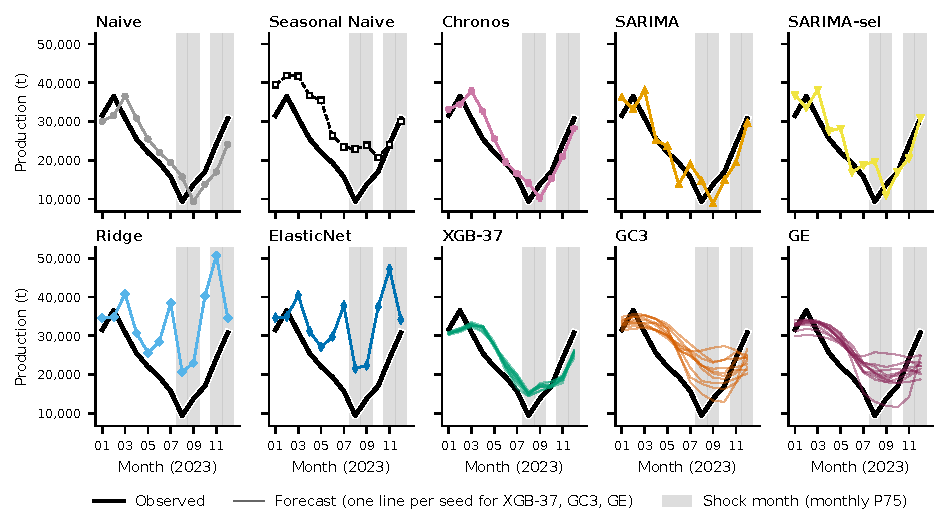
\includegraphics[width=\linewidth,height=0.36\textheight,keepaspectratio]{fig20_real_vs_pred_2023_sutil.pdf}
\caption{Sour lime, 2023}
\label{fig:fig20_real_vs_pred_2023_sutil}
\end{subfigure}
\par\medskip
\begin{subfigure}{\linewidth}
\centering
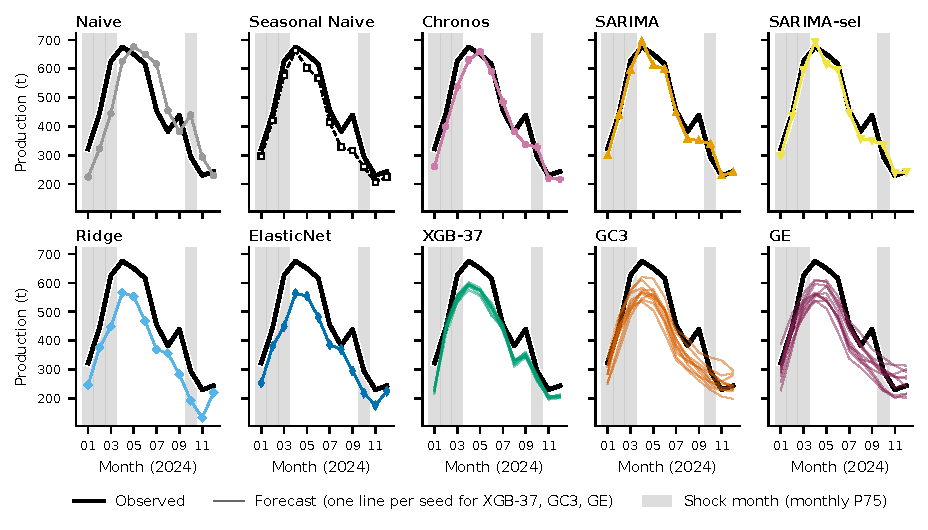
\includegraphics[width=\linewidth,height=0.36\textheight,keepaspectratio]{fig20_real_vs_pred_2024_dulce.pdf}
\caption{Sweet lime, 2024}
\label{fig:fig20_real_vs_pred_2024_dulce}
\end{subfigure}
\caption{\textit{Sour lime, 2023:} \figcap{fig20_real_vs_pred_2023_sutil} \textit{Sweet lime, 2024:} \figcap{fig20_real_vs_pred_2024_dulce}}
\label{fig:fig20_real_vs_pred_2023_sutil__fig20_real_vs_pred_2024_dulce}
\end{figure}

\begin{figure}[htbp]
\centering
\begin{subfigure}{\linewidth}
\centering
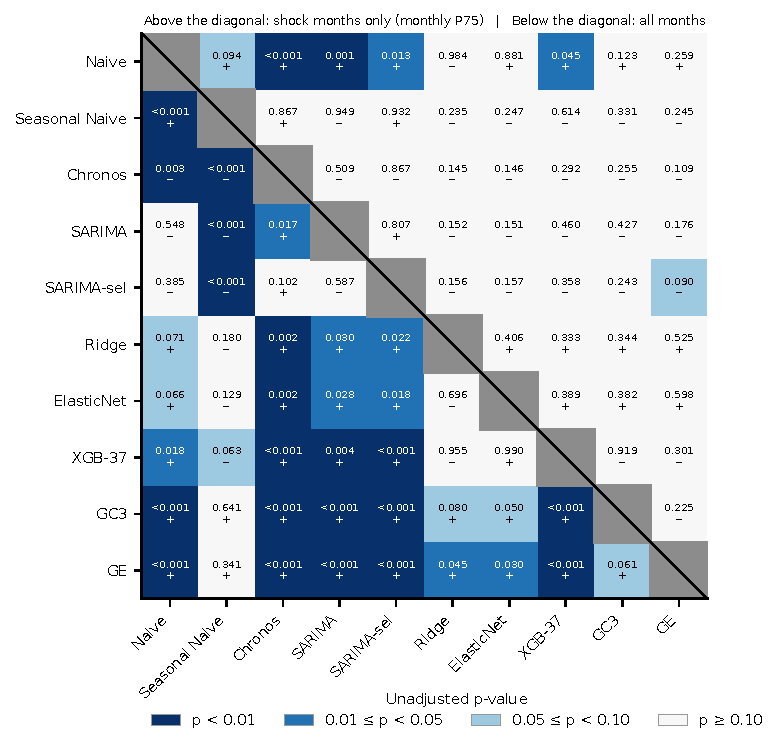
\includegraphics[width=\linewidth,height=0.36\textheight,keepaspectratio]{fig19_dm_pvalue_matrix_sutil.pdf}
\caption{Sour lime}
\label{fig:fig19_dm_pvalue_matrix_sutil}
\end{subfigure}
\par\medskip
\begin{subfigure}{\linewidth}
\centering
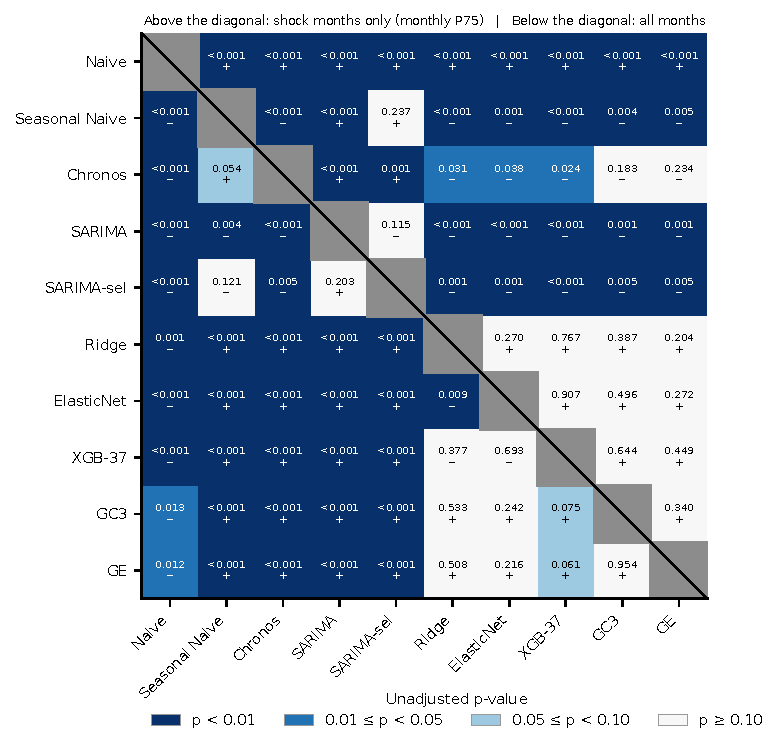
\includegraphics[width=\linewidth,height=0.36\textheight,keepaspectratio]{fig19_dm_pvalue_matrix_dulce.pdf}
\caption{Sweet lime}
\label{fig:fig19_dm_pvalue_matrix_dulce}
\end{subfigure}
\caption{\textit{Sour lime:} \figcap{fig19_dm_pvalue_matrix_sutil} \textit{Sweet lime:} \figcap{fig19_dm_pvalue_matrix_dulce}}
\label{fig:fig19_dm_pvalue_matrix}
\end{figure}

\begin{figure}[htbp]
\centering
\begin{subfigure}{\linewidth}
\centering
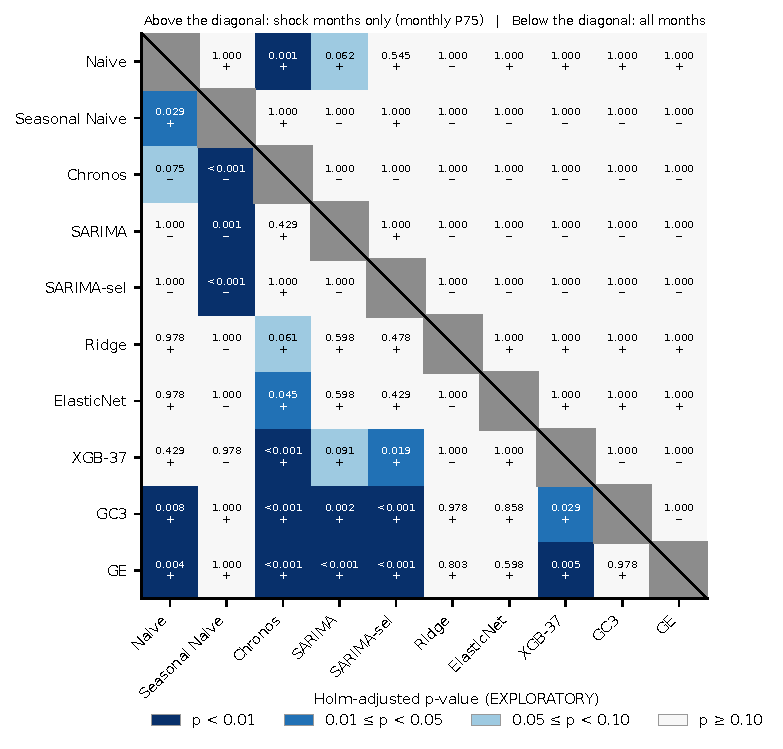
\includegraphics[width=\linewidth,height=0.36\textheight,keepaspectratio]{fig19b_dm_pvalue_matrix_holm_sutil.pdf}
\caption{Sour lime}
\label{fig:fig19b_dm_pvalue_matrix_holm_sutil}
\end{subfigure}
\par\medskip
\begin{subfigure}{\linewidth}
\centering
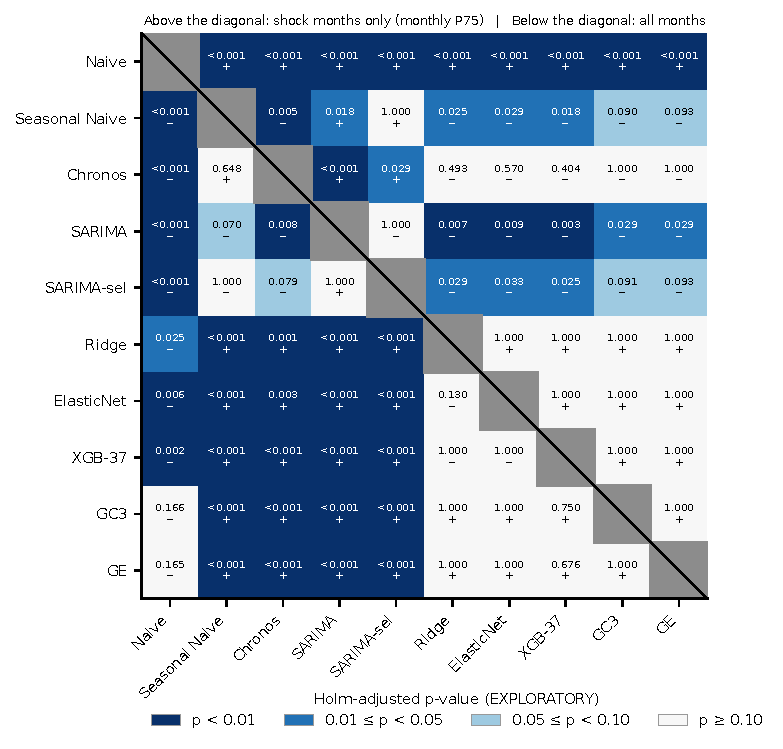
\includegraphics[width=\linewidth,height=0.36\textheight,keepaspectratio]{fig19b_dm_pvalue_matrix_holm_dulce.pdf}
\caption{Sweet lime}
\label{fig:fig19b_dm_pvalue_matrix_holm_dulce}
\end{subfigure}
\caption{\textbf{EXPLORATORY.} \textit{Sour lime:} \figcap{fig19b_dm_pvalue_matrix_holm_sutil} \textit{Sweet lime:} \figcap{fig19b_dm_pvalue_matrix_holm_dulce}}
\label{fig:fig19b_dm_pvalue_matrix_holm}
\end{figure}

\begin{figure}[htbp]
\centering
\begin{subfigure}{\linewidth}
\centering
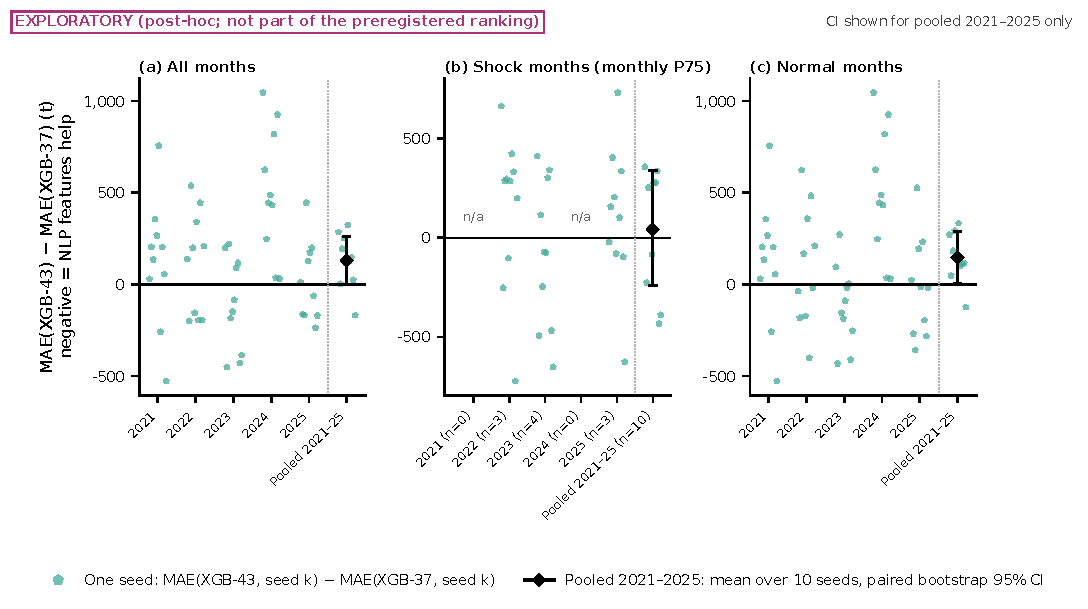
\includegraphics[width=\linewidth,height=0.36\textheight,keepaspectratio]{fig18b_xgb43_vs_xgb37_exploratory_sutil.pdf}
\caption{Sour lime}
\label{fig:fig18b_xgb43_vs_xgb37_exploratory_sutil}
\end{subfigure}
\par\medskip
\begin{subfigure}{\linewidth}
\centering
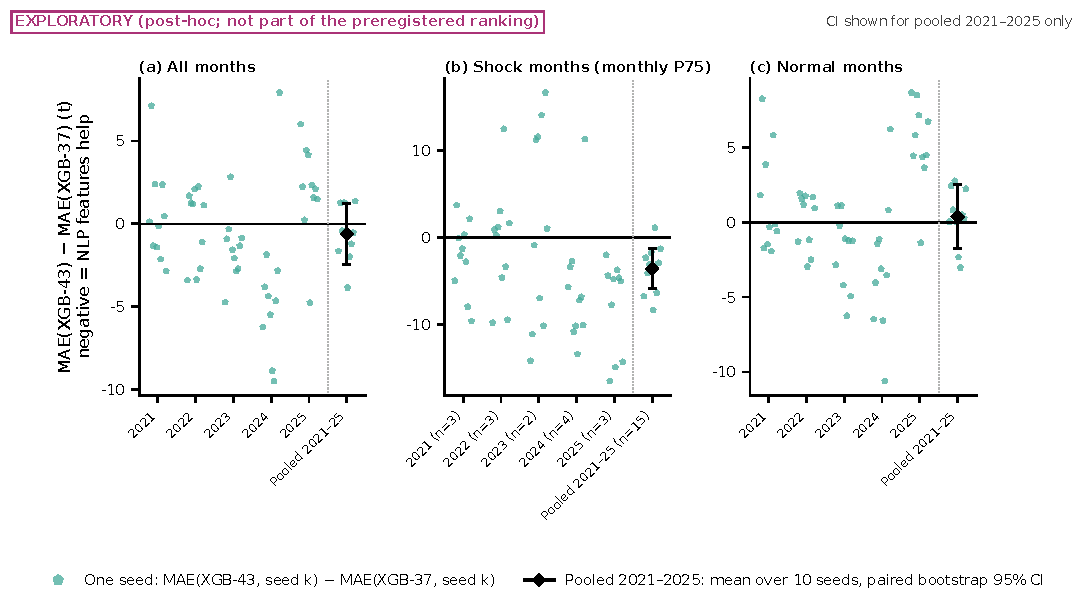
\includegraphics[width=\linewidth,height=0.36\textheight,keepaspectratio]{fig18b_xgb43_vs_xgb37_exploratory_dulce.pdf}
\caption{Sweet lime}
\label{fig:fig18b_xgb43_vs_xgb37_exploratory_dulce}
\end{subfigure}
\caption{\textit{Sour lime:} \figcap{fig18b_xgb43_vs_xgb37_exploratory_sutil} \textit{Sweet lime:} \figcap{fig18b_xgb43_vs_xgb37_exploratory_dulce}}
\label{fig:fig18b_xgb43_vs_xgb37_exploratory}
\end{figure}

\begin{figure}[htbp]
\centering
\begin{subfigure}{\linewidth}
\centering
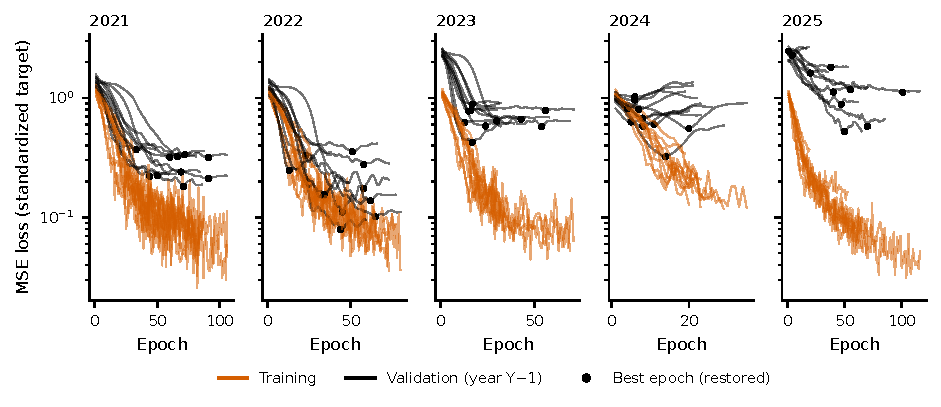
\includegraphics[width=\linewidth,height=0.36\textheight,keepaspectratio]{fig01_loss_curves_gc3_sutil.pdf}
\caption{Sour lime}
\label{fig:fig01_loss_curves_gc3_sutil}
\end{subfigure}
\par\medskip
\begin{subfigure}{\linewidth}
\centering
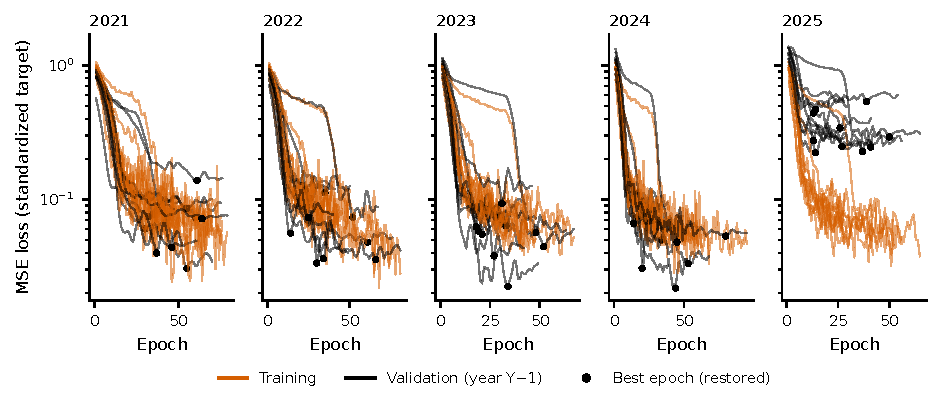
\includegraphics[width=\linewidth,height=0.36\textheight,keepaspectratio]{fig01_loss_curves_gc3_dulce.pdf}
\caption{Sweet lime}
\label{fig:fig01_loss_curves_gc3_dulce}
\end{subfigure}
\caption{\textit{Sour lime:} \figcap{fig01_loss_curves_gc3_sutil} \textit{Sweet lime:} \figcap{fig01_loss_curves_gc3_dulce}}
\label{fig:fig01_loss_curves_gc3}
\end{figure}

\begin{figure}[htbp]
\centering
\begin{subfigure}{\linewidth}
\centering
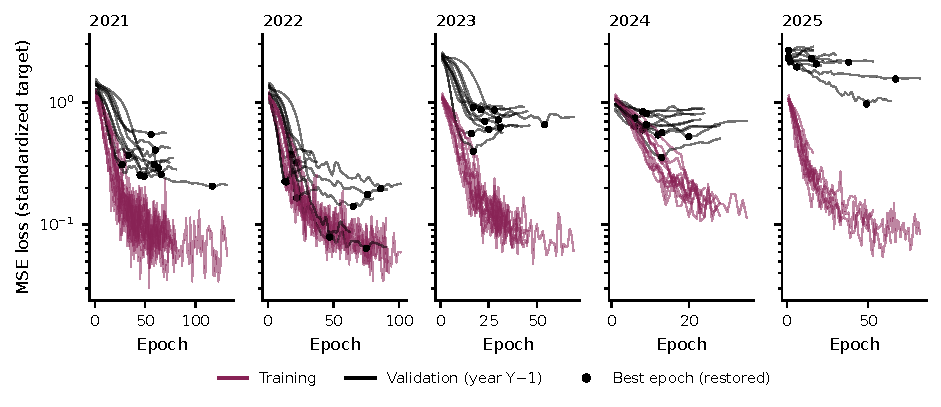
\includegraphics[width=\linewidth,height=0.36\textheight,keepaspectratio]{fig01_loss_curves_ge_sutil.pdf}
\caption{Sour lime}
\label{fig:fig01_loss_curves_ge_sutil}
\end{subfigure}
\par\medskip
\begin{subfigure}{\linewidth}
\centering
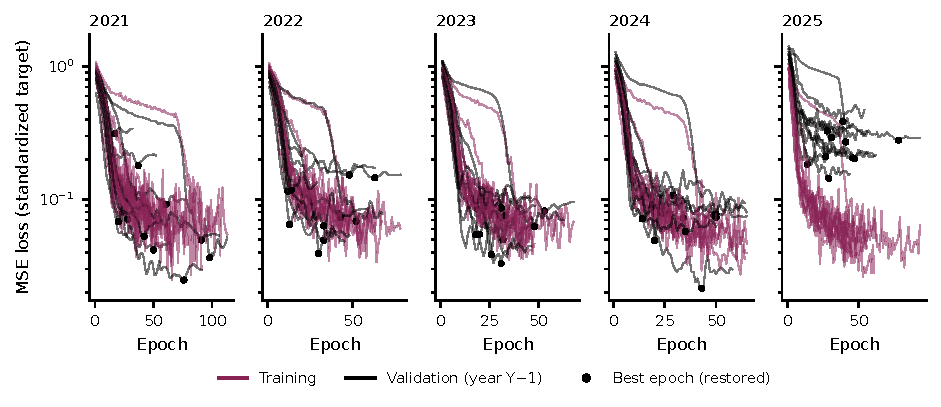
\includegraphics[width=\linewidth,height=0.36\textheight,keepaspectratio]{fig01_loss_curves_ge_dulce.pdf}
\caption{Sweet lime}
\label{fig:fig01_loss_curves_ge_dulce}
\end{subfigure}
\caption{\textit{Sour lime:} \figcap{fig01_loss_curves_ge_sutil} \textit{Sweet lime:} \figcap{fig01_loss_curves_ge_dulce}}
\label{fig:fig01_loss_curves_ge}
\end{figure}

\begin{figure}[htbp]
\centering
\begin{subfigure}{\linewidth}
\centering
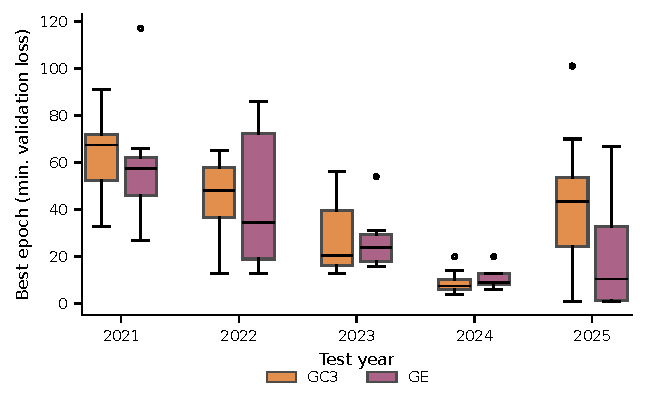
\includegraphics[width=\linewidth,height=0.36\textheight,keepaspectratio]{fig03_early_stopping_epoch_sutil.pdf}
\caption{Sour lime}
\label{fig:fig03_early_stopping_epoch_sutil}
\end{subfigure}
\par\medskip
\begin{subfigure}{\linewidth}
\centering
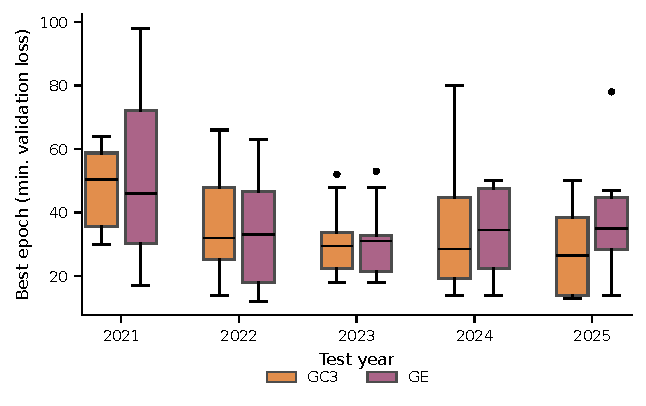
\includegraphics[width=\linewidth,height=0.36\textheight,keepaspectratio]{fig03_early_stopping_epoch_dulce.pdf}
\caption{Sweet lime}
\label{fig:fig03_early_stopping_epoch_dulce}
\end{subfigure}
\caption{\textit{Sour lime:} \figcap{fig03_early_stopping_epoch_sutil} \textit{Sweet lime:} \figcap{fig03_early_stopping_epoch_dulce}}
\label{fig:fig03_early_stopping_epoch}
\end{figure}

\begin{figure}[htbp]
\centering
\begin{subfigure}{\linewidth}
\centering
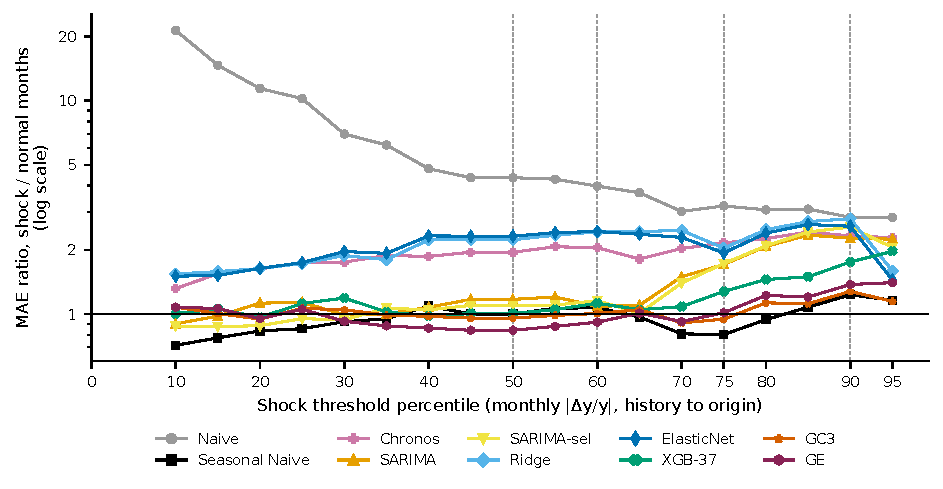
\includegraphics[width=\linewidth,height=0.36\textheight,keepaspectratio]{fig06_ratio_shock_normal_vs_percentile_sutil.pdf}
\caption{Sour lime}
\label{fig:fig06_ratio_shock_normal_vs_percentile_sutil}
\end{subfigure}
\par\medskip
\begin{subfigure}{\linewidth}
\centering
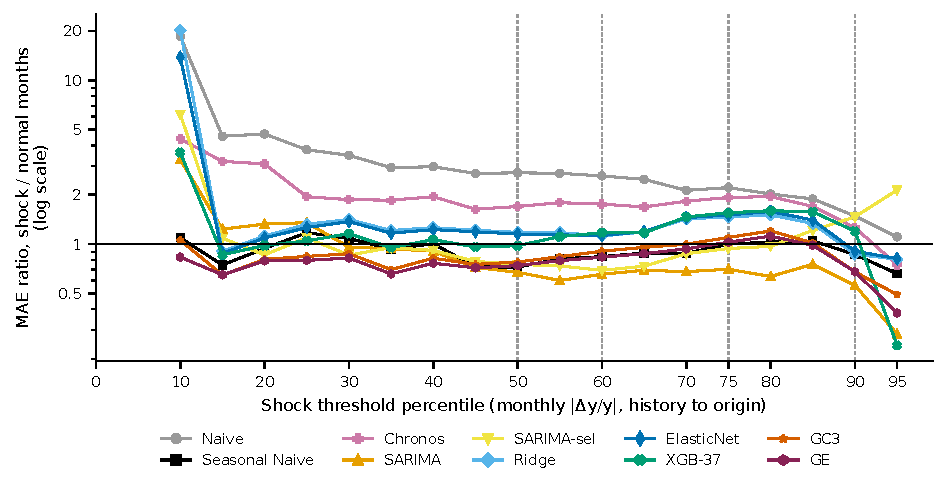
\includegraphics[width=\linewidth,height=0.36\textheight,keepaspectratio]{fig06_ratio_shock_normal_vs_percentile_dulce.pdf}
\caption{Sweet lime}
\label{fig:fig06_ratio_shock_normal_vs_percentile_dulce}
\end{subfigure}
\caption{\textit{Sour lime:} \figcap{fig06_ratio_shock_normal_vs_percentile_sutil} \textit{Sweet lime:} \figcap{fig06_ratio_shock_normal_vs_percentile_dulce}}
\label{fig:fig06_ratio_shock_normal_vs_percentile}
\end{figure}

\begin{figure}[htbp]
\centering
\begin{subfigure}{\linewidth}
\centering
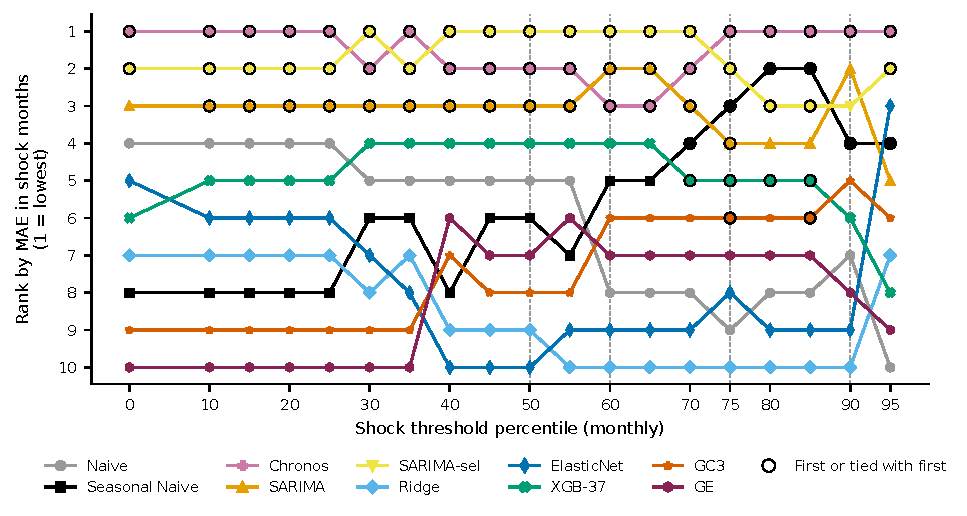
\includegraphics[width=\linewidth,height=0.36\textheight,keepaspectratio]{fig08_rank_bump_chart_sutil.pdf}
\caption{Sour lime}
\label{fig:fig08_rank_bump_chart_sutil}
\end{subfigure}
\par\medskip
\begin{subfigure}{\linewidth}
\centering
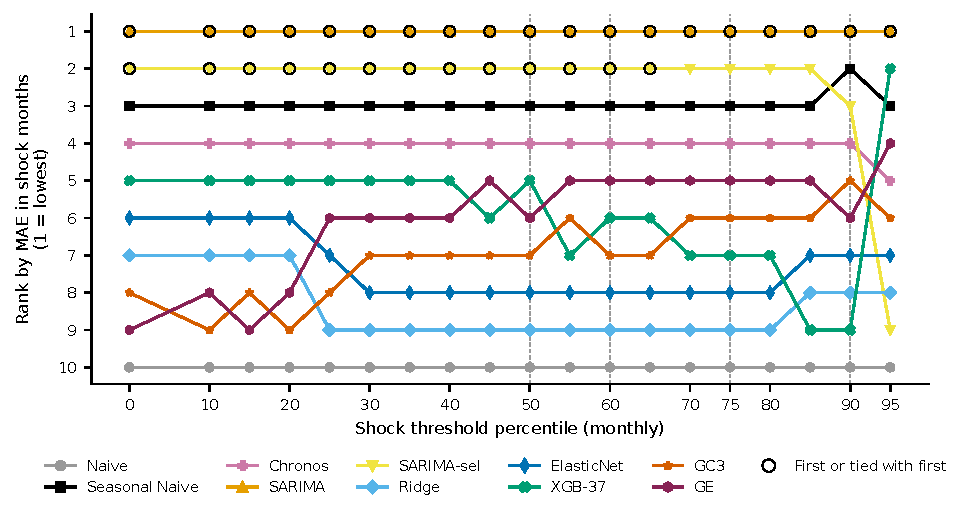
\includegraphics[width=\linewidth,height=0.36\textheight,keepaspectratio]{fig08_rank_bump_chart_dulce.pdf}
\caption{Sweet lime}
\label{fig:fig08_rank_bump_chart_dulce}
\end{subfigure}
\caption{\textit{Sour lime:} \figcap{fig08_rank_bump_chart_sutil} \textit{Sweet lime:} \figcap{fig08_rank_bump_chart_dulce}}
\label{fig:fig08_rank_bump_chart}
\end{figure}

\begin{figure}[htbp]
\centering
\begin{subfigure}{0.49\linewidth}
\centering
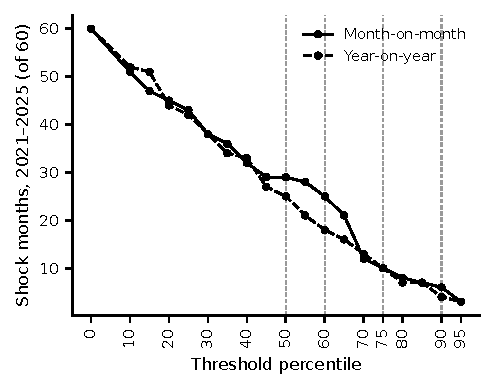
\includegraphics[width=\linewidth]{fig09_n_shock_vs_percentile_sutil.pdf}
\caption{Sour lime}
\label{fig:fig09_n_shock_vs_percentile_sutil}
\end{subfigure}\hfill
\begin{subfigure}{0.49\linewidth}
\centering
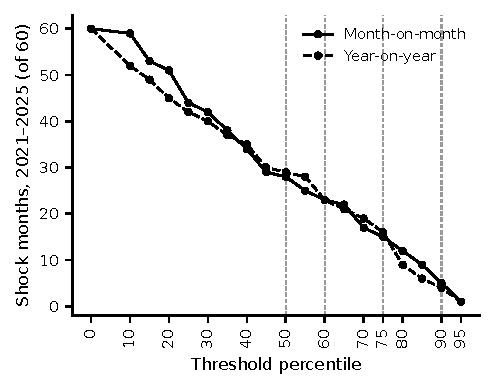
\includegraphics[width=\linewidth]{fig09_n_shock_vs_percentile_dulce.pdf}
\caption{Sweet lime}
\label{fig:fig09_n_shock_vs_percentile_dulce}
\end{subfigure}
\caption{\textit{Sour lime:} \figcap{fig09_n_shock_vs_percentile_sutil} \textit{Sweet lime:} \figcap{fig09_n_shock_vs_percentile_dulce}}
\label{fig:fig09_n_shock_vs_percentile}
\end{figure}

\begin{figure}[htbp]
\centering
\begin{subfigure}{\linewidth}
\centering
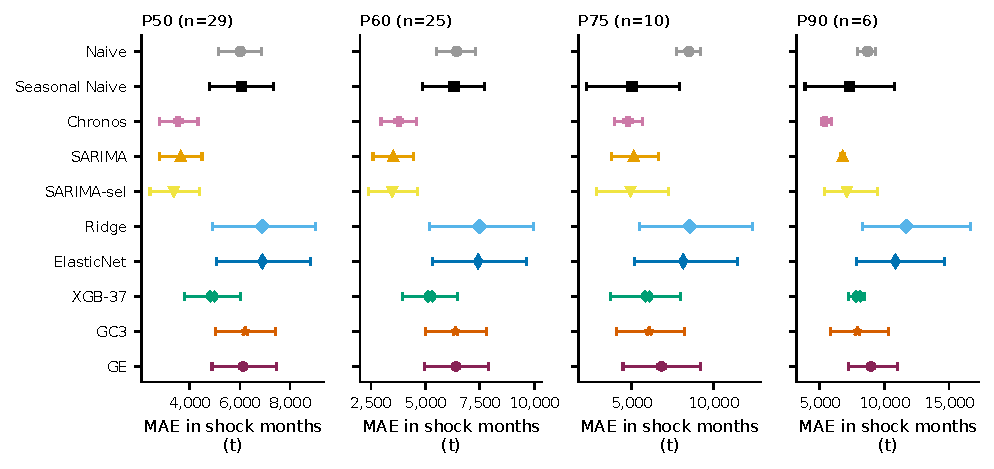
\includegraphics[width=\linewidth,height=0.36\textheight,keepaspectratio]{fig11_bootstrap_ci_mae_shock_report_points_sutil.pdf}
\caption{Sour lime}
\label{fig:fig11_bootstrap_ci_mae_shock_report_points_sutil}
\end{subfigure}
\par\medskip
\begin{subfigure}{\linewidth}
\centering
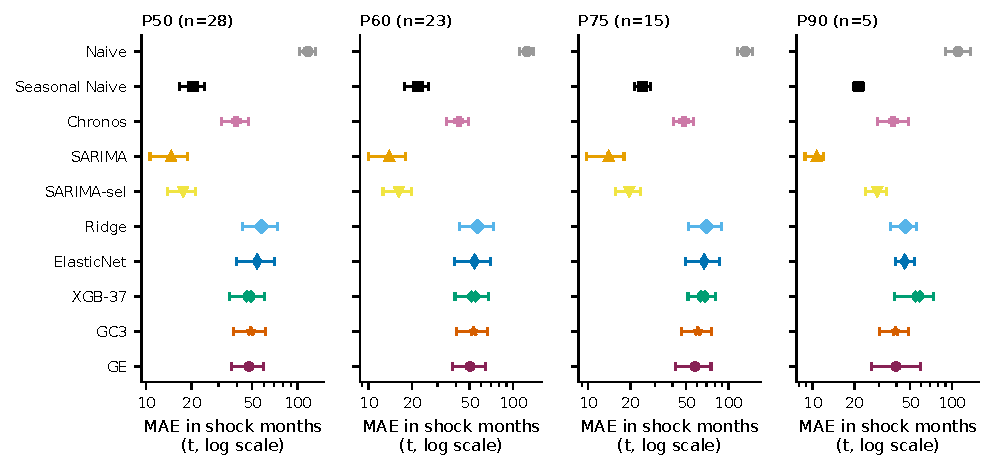
\includegraphics[width=\linewidth,height=0.36\textheight,keepaspectratio]{fig11_bootstrap_ci_mae_shock_report_points_dulce.pdf}
\caption{Sweet lime}
\label{fig:fig11_bootstrap_ci_mae_shock_report_points_dulce}
\end{subfigure}
\caption{\textit{Sour lime:} \figcap{fig11_bootstrap_ci_mae_shock_report_points_sutil} \textit{Sweet lime:} \figcap{fig11_bootstrap_ci_mae_shock_report_points_dulce}}
\label{fig:fig11_bootstrap_ci_mae_shock_report_points}
\end{figure}

\begin{figure}[htbp]
\centering
\begin{subfigure}{\linewidth}
\centering
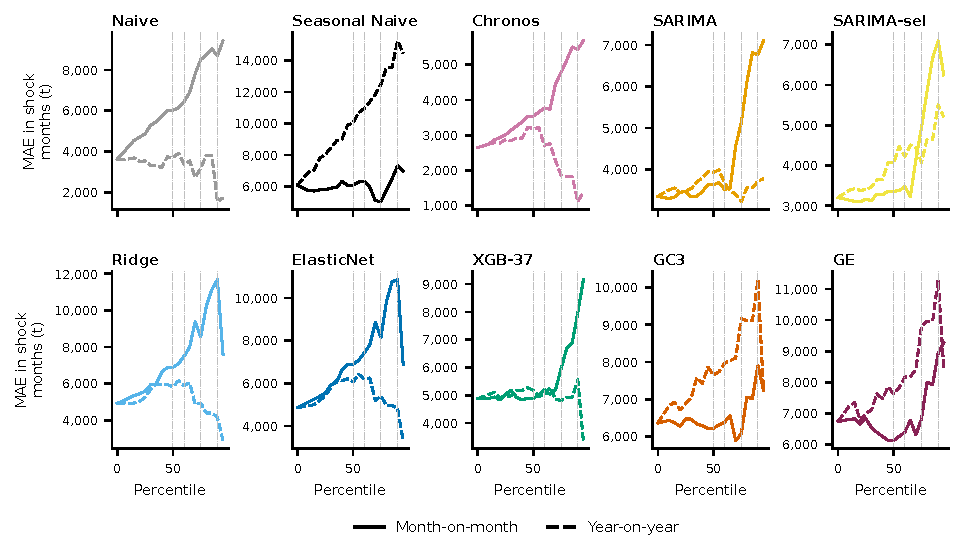
\includegraphics[width=\linewidth,height=0.36\textheight,keepaspectratio]{fig12_yoy_vs_mom_threshold_sutil.pdf}
\caption{Sour lime}
\label{fig:fig12_yoy_vs_mom_threshold_sutil}
\end{subfigure}
\par\medskip
\begin{subfigure}{\linewidth}
\centering
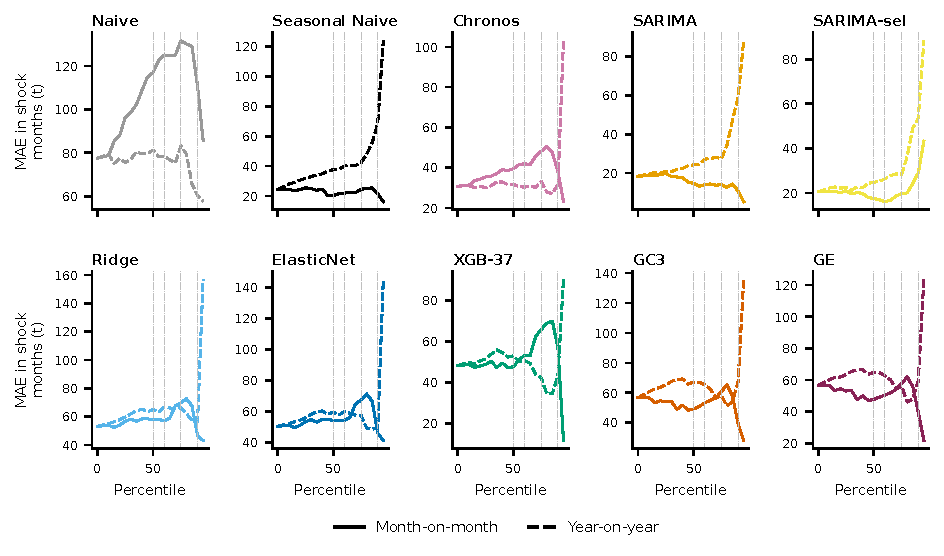
\includegraphics[width=\linewidth,height=0.36\textheight,keepaspectratio]{fig12_yoy_vs_mom_threshold_dulce.pdf}
\caption{Sweet lime}
\label{fig:fig12_yoy_vs_mom_threshold_dulce}
\end{subfigure}
\caption{\textit{Sour lime:} \figcap{fig12_yoy_vs_mom_threshold_sutil} \textit{Sweet lime:} \figcap{fig12_yoy_vs_mom_threshold_dulce}}
\label{fig:fig12_yoy_vs_mom_threshold}
\end{figure}

\begin{figure}[htbp]
\centering
\begin{subfigure}{\linewidth}
\centering
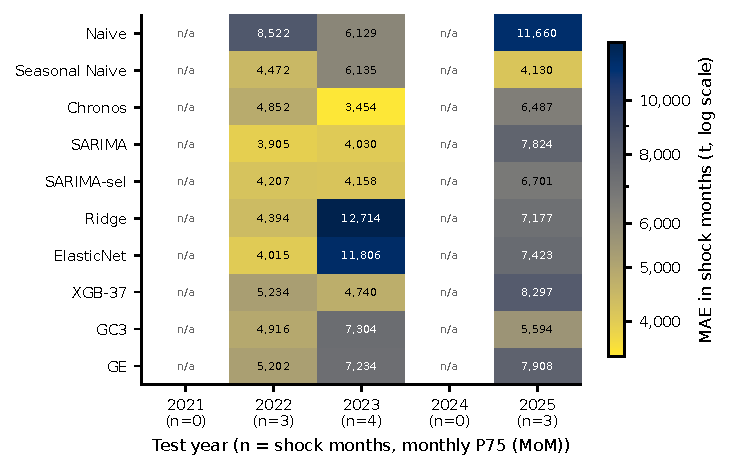
\includegraphics[width=\linewidth,height=0.36\textheight,keepaspectratio]{fig14_mae_shock_heatmap_model_window_sutil.pdf}
\caption{Sour lime}
\label{fig:fig14_mae_shock_heatmap_model_window_sutil}
\end{subfigure}
\par\medskip
\begin{subfigure}{\linewidth}
\centering
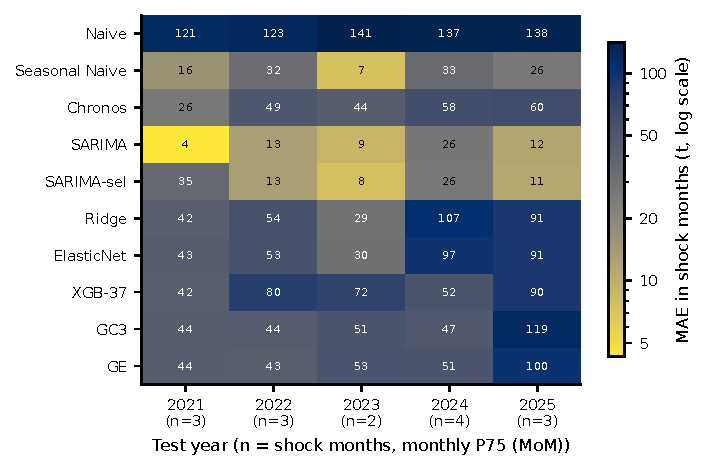
\includegraphics[width=\linewidth,height=0.36\textheight,keepaspectratio]{fig14_mae_shock_heatmap_model_window_dulce.pdf}
\caption{Sweet lime}
\label{fig:fig14_mae_shock_heatmap_model_window_dulce}
\end{subfigure}
\caption{\textit{Sour lime:} \figcap{fig14_mae_shock_heatmap_model_window_sutil} \textit{Sweet lime:} \figcap{fig14_mae_shock_heatmap_model_window_dulce}}
\label{fig:fig14_mae_shock_heatmap_model_window}
\end{figure}

\begin{figure}[htbp]
\centering
\begin{subfigure}{\linewidth}
\centering
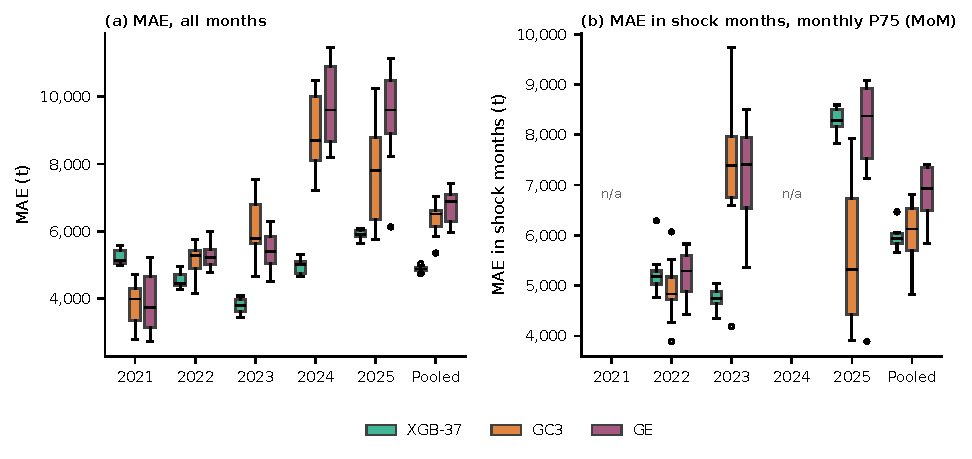
\includegraphics[width=\linewidth,height=0.36\textheight,keepaspectratio]{fig15_seed_boxplots_sutil.pdf}
\caption{Sour lime}
\label{fig:fig15_seed_boxplots_sutil}
\end{subfigure}
\par\medskip
\begin{subfigure}{\linewidth}
\centering
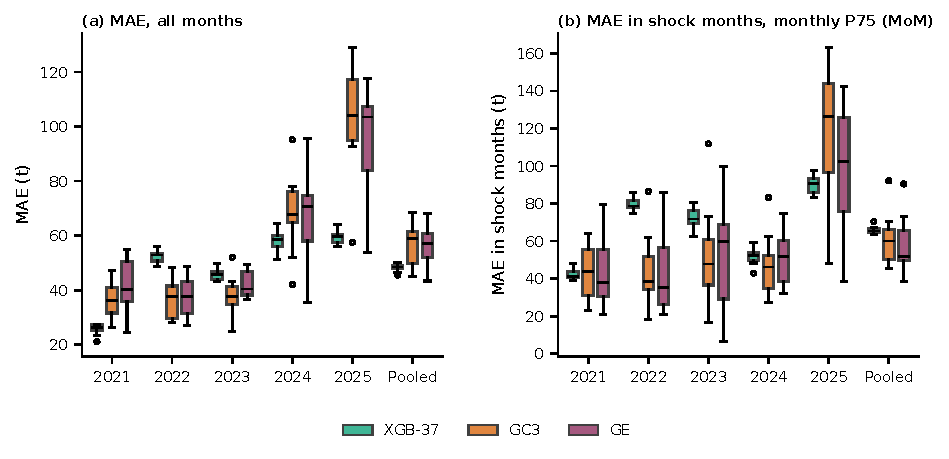
\includegraphics[width=\linewidth,height=0.36\textheight,keepaspectratio]{fig15_seed_boxplots_dulce.pdf}
\caption{Sweet lime}
\label{fig:fig15_seed_boxplots_dulce}
\end{subfigure}
\caption{\textit{Sour lime:} \figcap{fig15_seed_boxplots_sutil} \textit{Sweet lime:} \figcap{fig15_seed_boxplots_dulce}}
\label{fig:fig15_seed_boxplots}
\end{figure}

\begin{figure}[htbp]
\centering
\begin{subfigure}{\linewidth}
\centering
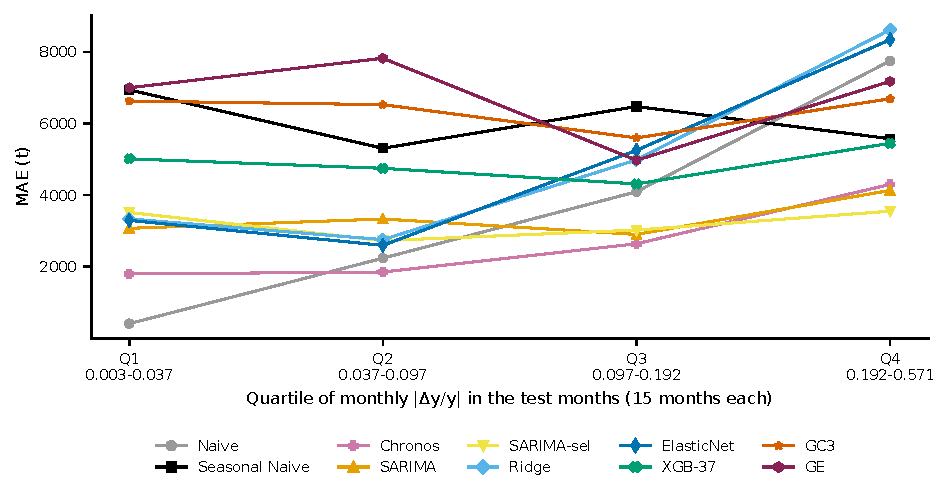
\includegraphics[width=\linewidth,height=0.36\textheight,keepaspectratio]{fig16_mae_by_change_quartile_sutil.pdf}
\caption{Sour lime}
\label{fig:fig16_mae_by_change_quartile_sutil}
\end{subfigure}
\par\medskip
\begin{subfigure}{\linewidth}
\centering
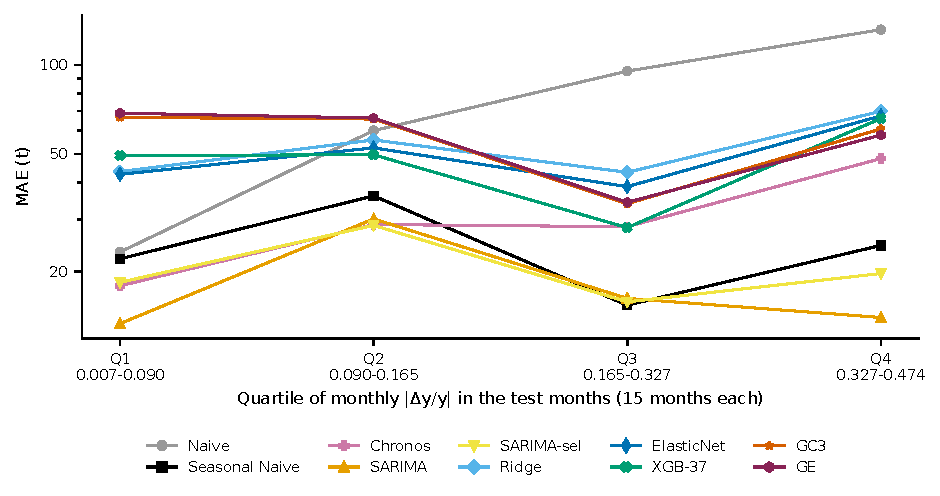
\includegraphics[width=\linewidth,height=0.36\textheight,keepaspectratio]{fig16_mae_by_change_quartile_dulce.pdf}
\caption{Sweet lime}
\label{fig:fig16_mae_by_change_quartile_dulce}
\end{subfigure}
\caption{\textit{Sour lime:} \figcap{fig16_mae_by_change_quartile_sutil} \textit{Sweet lime:} \figcap{fig16_mae_by_change_quartile_dulce}}
\label{fig:fig16_mae_by_change_quartile}
\end{figure}

\begin{figure}[htbp]
\centering
\begin{subfigure}{\linewidth}
\centering
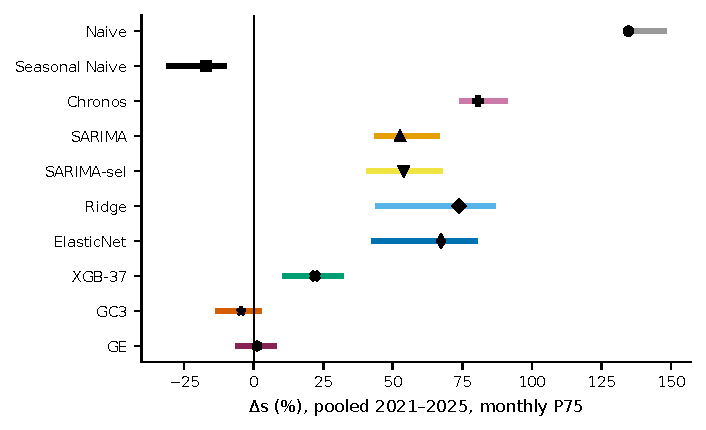
\includegraphics[width=\linewidth,height=0.36\textheight,keepaspectratio]{fig17_leave_one_shock_out_delta_s_sutil.pdf}
\caption{Sour lime}
\label{fig:fig17_leave_one_shock_out_delta_s_sutil}
\end{subfigure}
\par\medskip
\begin{subfigure}{\linewidth}
\centering
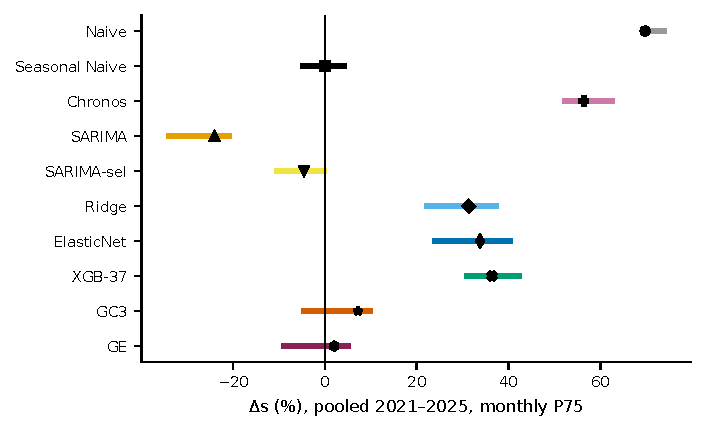
\includegraphics[width=\linewidth,height=0.36\textheight,keepaspectratio]{fig17_leave_one_shock_out_delta_s_dulce.pdf}
\caption{Sweet lime}
\label{fig:fig17_leave_one_shock_out_delta_s_dulce}
\end{subfigure}
\caption{\textit{Sour lime:} \figcap{fig17_leave_one_shock_out_delta_s_sutil} \textit{Sweet lime:} \figcap{fig17_leave_one_shock_out_delta_s_dulce}}
\label{fig:fig17_leave_one_shock_out_delta_s}
\end{figure}

\begin{figure}[htbp]
\centering
\begin{subfigure}{\linewidth}
\centering
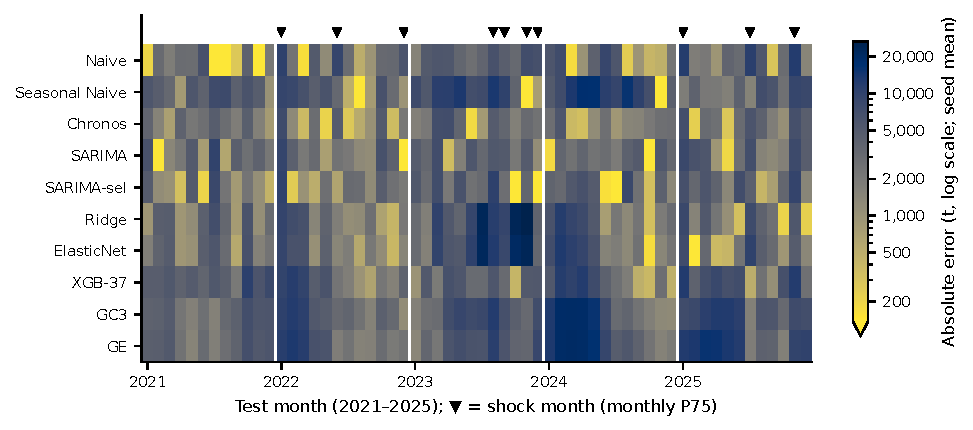
\includegraphics[width=\linewidth,height=0.36\textheight,keepaspectratio]{fig21_abs_error_monthly_sutil.pdf}
\caption{Sour lime}
\label{fig:fig21_abs_error_monthly_sutil}
\end{subfigure}
\par\medskip
\begin{subfigure}{\linewidth}
\centering
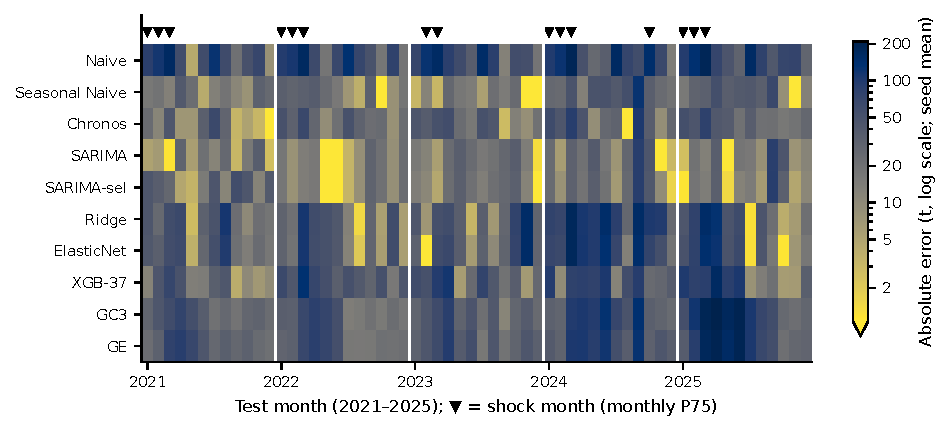
\includegraphics[width=\linewidth,height=0.36\textheight,keepaspectratio]{fig21_abs_error_monthly_dulce.pdf}
\caption{Sweet lime}
\label{fig:fig21_abs_error_monthly_dulce}
\end{subfigure}
\caption{\textit{Sour lime:} \figcap{fig21_abs_error_monthly_sutil} \textit{Sweet lime:} \figcap{fig21_abs_error_monthly_dulce}}
\label{fig:fig21_abs_error_monthly}
\end{figure}



% ============================================================
\section{Discussion}

\textbf{Parsimony and pretrained benchmarks.} The results do not support the idea that greater model capacity yields lower error when the training set is small. In sour lime the lowest errors came from Chronos, applied without local training, and from the two SARIMA variants; in sweet lime from SARIMA and SARIMA-sel, which exchanged the first place between the primary pool and the 2023--2025 sensitivity set without a significant difference between them. The DualLSTM variants had the highest error of the ten models in sour lime and were clearly outperformed in sweet lime by the statistical models, the Seasonal Naive and the pretrained model; in sour lime their disadvantage against Chronos and both SARIMA variants was significant even after the Holm adjustment. This agrees with evidence that statistical and regularised methods are demanding benchmarks in short series~\cite{makridakis2020m4,hewamalage2021rnn,rather2024breaking} and indicates that a specialised architecture should be compared with them, and with pretrained models such as Chronos, TimesFM or Moirai~\cite{ansari2024chronos,das2024decoder,woo2024unified}, before being proposed for operational use. That a zero-shot univariate model ranked first in sour lime also suggests that, with about 40 to 90 training months, the exogenous context did not compensate for the extra parameters it requires.

\textbf{Overall versus shock-conditional evaluation.} Restricting the evaluation to shock months did not favour the DualLSTM. Its low $\Delta_s$ in sour lime ($-4.5$\% for GC3) reflects a high error in all months, not a low error in shock months: $\Delta_s$ is a ratio, and a model that is poor in every month can show a small penalty. The same applies to the Seasonal Naive ($\Delta_s=-17.1$\%). Reporting $\Delta_s$ alone would have ranked these models as the most resilient, whereas in absolute terms Chronos, SARIMA and SARIMA-sel were better in shock months as well. We therefore recommend reporting $\Delta_s$ only together with the absolute errors in shock and normal months. The shock-only comparisons rest on 10 and 15 months (7 and 9 in the sensitivity set) and have low power: in sour lime five models were statistically tied with the first at P75, and after the Holm adjustment only the comparison of Chronos with the Naive forecast remained. The ranking in shock months should therefore be read as a complementary diagnostic and not as evidence of intrinsic resilience. The choice between month-on-month and year-on-year changes also matters: under the year-on-year definition the Naive forecast became robust in sour lime, so the shock definition should be stated explicitly and its sensitivity reported.

\textbf{Contribution of news text.} News features did not improve the DualLSTM: they increased the error in sour lime and made no difference over all months in sweet lime. The only favourable signals are lower shock-month errors in sweet lime, for GE in the 2023--2025 sensitivity set and for XGB-43 in a post hoc analysis outside the ranking. Both rest on 9 to 15 months, and the first was not confirmed by the Diebold--Mariano test on seed-averaged errors. Overall, there is not enough evidence to claim that the text channel improves accuracy in this setting. Sentiment was computed zero-shot with a general-purpose model, and a model fitted to agricultural news could behave differently.

\textbf{Limitations.} The evaluation uses two related national series and five retrospective test windows (60 pooled months), which are not independent test sets; the test year 2025 had already been inspected in earlier experiments, and the order of the fixed sour-lime SARIMA was adopted after seeing it (Section~\ref{sec:transparency}). Shock months are few (10 and 15), the confidence intervals are wide and several pairwise differences cannot be separated from zero; $\Delta_s$, RMSE and MASE are reported without confidence intervals. The networks were run with fixed hyperparameters and no search, which may disadvantage them relative to models whose penalties or orders were re-chosen in each window. Chronos uses only the univariate history, whereas the DualLSTM receives multimodal variables, so the comparison concerns predictive performance and not equal information sets. The conversion of the MIDAGRI spreadsheet and of the INDECI records into the frozen tables has no code in the repository. The attention weights of the DualLSTM should not be interpreted as causal relations between climate, emergencies or news and production~\cite{jain2019attention}. A confirmatory evaluation on months not yet observed when the protocol was written, such as 2026, would address the main limitation of this study.

\section{Conclusions}

A DualLSTM with attention that separates the production history from the lagged exogenous context did not consistently outperform statistical, regularised, tree-based or pretrained benchmarks in the monthly forecasting of sour lime and sweet lime production in Peru under a rolling-origin evaluation with 60 test months per crop. The best model depended on the crop: Chronos, SARIMA and SARIMA-sel in sour lime, and SARIMA in sweet lime, where it was the only model first or tied at all four shock thresholds and remained statistically indistinguishable from SARIMA-sel, which ranked first in the 2023--2025 sensitivity set. The low shock penalty of the DualLSTM was explained by high errors in all months, so $\Delta_s$ must be reported together with the absolute errors. News-derived variables showed no consistent benefit. Future work should extend the analysis to more crops and regions, longer evaluation periods and independently documented external events, and should test networks with hyperparameter search.

\vspace{6pt}

% BORRADOR: confirmar con los coautores antes del envio
\authorcontributions{Conceptualization, F.Y.A.S.S., A.C.J. and E.T.-C.; methodology, F.Y.A.S.S. and E.T.-C.; software, F.Y.A.S.S.; validation, F.Y.A.S.S. and A.C.J.; formal analysis, F.Y.A.S.S.; investigation, F.Y.A.S.S. and A.C.J.; data curation, F.Y.A.S.S.; writing---original draft preparation, F.Y.A.S.S.; writing---review and editing, A.C.J. and E.T.-C.; visualization, F.Y.A.S.S.; supervision, E.T.-C. All authors have read and agreed to the published version of the manuscript.}
% BORRADOR: confirmar con el asesor si la UPeU financio tambien la investigacion
\funding{This research received no external funding. The article processing charge was funded by Universidad Peruana Uni\'on.}
\dataavailability{The national production series were built from the MIDAGRI SISAGRI Regional Productive Profile dashboard~\cite{midagri2026perfil}, climate data from NASA POWER, emergency records from INDECI and news from Agraria.pe. The frozen tables derived from these sources, with their SHA-256 hashes, and the code are available at \url{https://github.com/YeralD21/Machine-Learning-Multimodal--Agro-NLP-Clima-} (release \texttt{v2.0-forecasting}).}
\conflictsofinterest{The authors declare no conflicts of interest.}

\appendixtitles{yes}
\appendixstart
\appendix
\input{secciones/A_practicas_semilla}

\begin{adjustwidth}{-\extralength}{0cm}
\reftitle{References}
\bibliography{referencias}
\PublishersNote{}
\end{adjustwidth}
\end{document}